\documentclass[a4paper,12pt,oneside]{report}

\usepackage[utf8]{inputenc}
\usepackage[T1]{fontenc}
\usepackage{csquotes}
\usepackage[french]{babel}

\usepackage[
  top=2.5cm,
  bottom=2.5cm,
  left=3cm,
  right=2.5cm,
  headheight=14.5pt
]{geometry}

\usepackage{lmodern}
\usepackage{microtype}
\usepackage{setspace}
\onehalfspacing

\usepackage[dvipsnames,table]{xcolor}
\definecolor{TynassBlue}{RGB}{0,72,255}
\definecolor{TynassLight}{RGB}{152,181,255}
\definecolor{TynassDark}{RGB}{0,42,153}
\definecolor{LightGray}{RGB}{245,247,255}
\definecolor{MustColor}{RGB}{220,38,38}
\definecolor{ShouldColor}{RGB}{234,88,12}
\definecolor{CouldColor}{RGB}{22,163,74}

\usepackage{amsmath}
\usepackage{amssymb}

\usepackage{graphicx}
\usepackage{float}
\usepackage{caption}
\usepackage{subcaption}
\graphicspath{{./images/}}

\usepackage{booktabs}
\usepackage{tabularx}
\usepackage{multirow}
\usepackage{multicol}
\usepackage{longtable}
\usepackage{array}
\usepackage{makecell}
\renewcommand{\arraystretch}{1.4}

\usepackage{enumitem}
\setlist[itemize]{noitemsep, topsep=4pt}
\setlist[enumerate]{noitemsep, topsep=4pt}

\usepackage{listings}
\lstset{
  basicstyle=\ttfamily\small,
  backgroundcolor=\color{LightGray},
  frame=single,
  rulecolor=\color{TynassLight},
  breaklines=true,
  breakatwhitespace=true,
  numbers=left,
  numberstyle=\tiny\color{gray},
  keywordstyle=\color{TynassBlue}\bfseries,
  commentstyle=\color{gray}\itshape,
  stringstyle=\color{TynassDark},
  tabsize=2,
  showstringspaces=false,
  captionpos=b,
  inputencoding=utf8,
  extendedchars=true,
  literate=
    {é}{{\'e}}1 {è}{{\`e}}1 {ê}{{\^e}}1 {à}{{\`a}}1
    {ù}{{\`u}}1 {ô}{{\^o}}1 {î}{{\^i}}1 {ç}{{\c c}}1
    {â}{{\^a}}1 {û}{{\^u}}1 {É}{{\'E}}1 {È}{{\`E}}1
    {Ê}{{\^E}}1 {À}{{\`A}}1 {Ù}{{\`U}}1 {Ô}{{\^O}}1
    {Î}{{\^I}}1 {Ç}{{\c C}}1 {Â}{{\^A}}1 {Û}{{\^U}}1
}

\usepackage{fancyhdr}
\pagestyle{fancy}
\fancyhf{}
\fancyhead[L]{\small\textit{\leftmark}}
\fancyhead[R]{\small\textcolor{TynassBlue}{\textbf{TynassIt}}}
\fancyfoot[C]{\thepage}
\renewcommand{\headrulewidth}{0.4pt}
\renewcommand{\footrulewidth}{0pt}

\usepackage[
  colorlinks=true,
  linkcolor=TynassBlue,
  citecolor=TynassDark,
  urlcolor=TynassBlue,
  pdftitle={TynassIt --- Rapport PFE},
  pdfsubject={Plateforme B2B de Formation en Réalité Virtuelle}
]{hyperref}
\usepackage{bookmark}

\usepackage[
  backend=biber,
  style=numeric,
  sorting=none,
  citestyle=numeric-comp
]{biblatex}
\addbibresource{references.bib}

\usepackage{tcolorbox}
\tcbuselibrary{skins,breakable}

\newtcolorbox{archbox}{
  colback=LightGray,
  colframe=TynassBlue,
  fonttitle=\bfseries\color{white},
  title=D\'{e}cision architecturale,
  arc=4pt,
  boxrule=1pt,
  breakable
}

\newtcolorbox{ucbox}[1]{
  colback=LightGray,
  colframe=TynassDark,
  fonttitle=\bfseries\color{white},
  title=Cas d'utilisation : #1,
  arc=4pt,
  boxrule=1pt,
  breakable
}

\newtcolorbox{notebox}{
  colback=yellow!10,
  colframe=orange!70,
  fonttitle=\bfseries,
  title=Note,
  arc=4pt,
  boxrule=1pt,
  breakable
}

\newcommand{\tynassit}{\textcolor{TynassBlue}{\textbf{TynassIt}}}
\newcommand{\must}{\textcolor{MustColor}{\textbf{Must}}}
\newcommand{\should}{\textcolor{ShouldColor}{\textbf{Should}}}
\newcommand{\could}{\textcolor{CouldColor}{\textbf{Could}}}
\newcommand{\wont}{\textcolor{gray}{\textbf{Won't}}}
\newcommand{\placeholder}[1]{
  \begin{center}
    \fbox{\parbox{0.8\textwidth}{
      \centering\vspace{0.8cm}
      \textit{\textcolor{gray}{[FIGURE~: #1]}}\\
      \vspace{0.8cm}
    }}
  \end{center}
}
\newcommand{\ok}{\textcolor{CouldColor}{\checkmark}}

\setlength{\emergencystretch}{3em}
\setcounter{secnumdepth}{3}
\setcounter{tocdepth}{3}

\begin{document}

\pagenumbering{roman}

\begin{titlepage}
\thispagestyle{empty}
\definecolor{coverblue}{RGB}{24,61,93}
\definecolor{covergray}{RGB}{84,92,101}
\begin{center}
\sffamily
\begin{minipage}{\textwidth}
    \centering
    {\color{coverblue}\rule{\linewidth}{1pt}}\\[0.3cm]
    {\color{covergray}\small\MakeUppercase{République Tunisienne}}\\[0.25cm]
    {\color{coverblue}\large\bfseries
    Ministère de l'Enseignement Supérieur et de la Recherche Scientifique}\\[0.25cm]
    {\large\bfseries Université de la Manouba}\\[0.15cm]
    {\large Institut Supérieur des Arts Multimédia de la Manouba}\\[0.3cm]
    {\color{coverblue}\rule{\linewidth}{1pt}}
    \vspace{0.45cm}
    
\includegraphics[width=0.32\textwidth]{../images/isamm_logo.png}
\end{minipage}
\vspace{0.65cm}
{\color{covergray}\Large\bfseries Rapport de Projet de Fin d'Études}\\[0.35cm]
{\normalsize Présenté en vue de l'obtention du diplôme de}\\[0.15cm]
{\color{coverblue}\large\bfseries Diplôme d'Ingénieur en Informatique et Multimédia}\\[0.15cm]
{\normalsize Spécialité : Image Numérique et Réalité Virtuelle}
\vspace{0.75cm}
{\color{coverblue}\rule{1\textwidth}{1.2pt}}\\[0.35cm]
{\color{coverblue}\LARGE\bfseries Conception et développement d'une plateforme B2B de formation en Réalité Virtuelle}\\[0.35cm]
{\color{coverblue}\rule{1\textwidth}{1.2pt}}
\vspace{1.5cm}
{\color{covergray}\slshape Réalisé par}\\[0.3cm]
{\large\bfseries Konte Skander}\\[0.18cm]
\vspace{0.65cm}
{\color{covergray}\slshape Encadré par}\\[0.3cm]
{\bfseries Hosni Ajlani} {\color{covergray}-- ISAMM}\\[0.18cm]
{\bfseries Med Ali Ezzeddine et Karim Hermi} {\color{covergray}-- Tynass IT}
\vfill
{\color{coverblue}\rule{1\textwidth}{1pt}}\\[0.3cm]
{\large\bfseries Année universitaire 2025--2026}
\end{center}
\end{titlepage}
\chapter*{Dédicaces}
\addcontentsline{toc}{chapter}{Dédicaces}
\markboth{Dédicaces}{}

\vspace{2cm}

\begin{flushright}
  \textit{[À compléter]}
\end{flushright}

\clearpage

\chapter*{Remerciements}
\addcontentsline{toc}{chapter}{Remerciements}
\markboth{Remerciements}{}

\vspace{1cm}

[À compléter]

\clearpage

\chapter*{R\'{e}sum\'{e}}
\addcontentsline{toc}{chapter}{R\'{e}sum\'{e}}
\markboth{R\'{e}sum\'{e}}{}

\vspace{0.5cm}

Ce projet de fin d'\'{e}tudes, r\'{e}alis\'{e} au sein de \textbf{Tynass IT},
porte sur la conception et le d\'{e}veloppement de \textbf{\tynassit{}},
une plateforme B2B d\'{e}di\'{e}e \`{a} la gestion et \`{a} la diffusion
de formations professionnelles en R\'{e}alit\'{e} Virtuelle (VR)
sur le casque \textbf{Meta Quest~3}.

La plateforme repose sur trois composantes compl\'{e}mentaires~:
un \textbf{backend REST} d\'{e}velopp\'{e} avec Node.js, Express et MongoDB Atlas~;
deux \textbf{dashboards web} d\'{e}velopp\'{e}s avec React et TypeScript~;
et une \textbf{application VR Unity~6} d\'{e}ploy\'{e}e sur Meta Quest~3,
permettant aux employ\'{e}s de vivre des simulations immersives de formation.

Dans le cadre du premier client, \textbf{Indigo Company}, un module
d'int\'{e}gration des nouveaux employ\'{e}s a \'{e}t\'{e} d\'{e}velopp\'{e}~:
exploration des locaux, pr\'{e}sentation des r\`{e}gles internes et
mises en situation sous forme de quiz, avec envoi automatique des
r\'{e}sultats vers la plateforme.

\textbf{Mots-cl\'{e}s~:} R\'{e}alit\'{e} Virtuelle, VR, B2B, formation
professionnelle, Meta Quest~3, Unity~6, Node.js, React, MongoDB, JWT, PFE.

\clearpage


\tableofcontents
\clearpage

\listoffigures
\addcontentsline{toc}{chapter}{Liste des figures}
\clearpage

\listoftables
\addcontentsline{toc}{chapter}{Liste des tableaux}
\clearpage

\chapter*{Liste des abréviations}
\addcontentsline{toc}{chapter}{Liste des abréviations}
\markboth{Liste des abréviations}{}

\vspace{0.5cm}

\begin{longtable}{p{3cm}p{\dimexpr\textwidth-3cm-4\tabcolsep\relax}}
  \toprule
  \textbf{Abréviation} & \textbf{Signification} \\
  \midrule
  \endfirsthead
  \toprule
  \textbf{Abréviation} & \textbf{Signification} \\
  \midrule
  \endhead
  \bottomrule
  \endfoot
  API    & Application Programming Interface \\
  APK    & Android Package \\
  AR     & Augmented Reality (Réalité Augmentée) \\
  B2B    & Business to Business \\
  BDD    & Base de Données \\
  CRUD   & Create, Read, Update, Delete \\
  EP     & Épic (Epic) \\
  FPS    & Frames Per Second \\
  HTTP   & HyperText Transfer Protocol \\
  JWT    & JSON Web Token \\
  LMS    & Learning Management System \\
  MoSCoW & Must, Should, Could, Won't \\
  MR     & Mixed Reality (Réalité Mixte) \\
  MVC    & Modèle-Vue-Contrôleur \\
  ODM    & Object Document Mapper \\
  PFE    & Projet de Fin d'Études \\
  PIN    & Personal Identification Number \\
  RBAC   & Role-Based Access Control \\
  REST   & Representational State Transfer \\
  SDK    & Software Development Kit \\
  SHA    & Secure Hash Algorithm \\
  SLA    & Service Level Agreement \\
  SQL    & Structured Query Language \\
  UI     & User Interface \\
  UML    & Unified Modeling Language \\
  URP    & Universal Render Pipeline \\
  US     & User Story \\
  UX     & User Experience \\
  VR     & Virtual Reality (Réalité Virtuelle) \\
  XR     & Extended Reality (Réalité Étendue) \\
\end{longtable}

\clearpage

\pagenumbering{arabic}
\setcounter{page}{1}

\chapter*{Introduction générale}
\addcontentsline{toc}{chapter}{Introduction générale}
\markboth{Introduction générale}{}

Dans un contexte de transformation numérique accélérée, les entreprises cherchent à
moderniser leurs processus de formation professionnelle. Les méthodes traditionnelles
~--- formations présentielles coûteuses, modules e-learning peu engageants~--- peinent à
répondre aux exigences d'efficacité et de standardisation des organisations modernes.
La Réalité Virtuelle (VR) émerge comme une réponse concrète à ces limites~: des études
empiriques indiquent que la formation en VR améliore la rétention des informations de
70~\% et rend les apprenants 4~fois plus rapides qu'une formation classique~\cite{pwc2020},
ce qui justifie son intégration dans les parcours de formation professionnelle B2B.

Le potentiel pédagogique de la VR étant établi, son adoption effective par les entreprises
se heurte toutefois à des obstacles concrets. Les solutions immersives disponibles sont
soit trop génériques~--- conçues indépendamment des procédures réelles d'une organisation
donnée~---, soit développées sur mesure pour un client unique, sans plateforme de gestion
permettant à l'entreprise de déployer la formation, d'en contrôler les accès et d'en
mesurer objectivement les résultats. Dans les deux cas, l'entreprise cliente reste sans
visibilité sur la progression réelle de ses collaborateurs, ce qui prive la formation de
la standardisation et de la traçabilité qu'elle devrait apporter. Le défi ne consiste
donc pas seulement à produire une expérience VR convaincante, mais à l'intégrer dans une
chaîne complète, de la gestion administrative des entreprises clientes jusqu'à la
restitution mesurable des performances de chaque employé~: comment concevoir une plateforme
B2B qui propose des formations professionnelles immersives en Réalité Virtuelle tout en
offrant aux entreprises les moyens de gérer leurs employés et de suivre objectivement leurs
performances~?

C'est à cette question que répond \tynassit{}, développée par Tynass~IT dans le cadre de
ce projet de fin d'études~: une plateforme B2B permettant aux entreprises clientes d'accéder
à des formations professionnelles immersives sur le casque Meta~Quest~3. Elle repose sur
trois composantes complémentaires. Un backend REST (Node.js, Express, MongoDB~Atlas) assure
l'authentification sécurisée, la gestion des accès et le suivi des sessions de formation.
Deux tableaux de bord web (React, TypeScript) offrent, l'un aux équipes Tynass la gestion
des entreprises et des modules VR, l'autre aux entreprises clientes la gestion de leurs
employés et la consultation des résultats. Enfin, une application VR déployée sur
Meta~Quest~3 permet aux employés d'effectuer des simulations immersives avec suivi
automatique des performances. Le premier module développé concerne l'intégration des
nouveaux employés d'Indigo~Company, leader tunisien du prêt-à-porter.

Ce rapport est organisé en six chapitres. Le premier présente le contexte général du
projet, une étude des solutions existantes, le choix de la méthodologie de travail~---
une approche Agile, itérative et incrémentale~--- ainsi que l'environnement de
développement. Le deuxième chapitre est consacré à la spécification des besoins et au
pilotage du projet. Les quatre chapitres suivants détaillent les quatre itérations de
développement réalisées, chacune apportant de nouvelles fonctionnalités à la plateforme~:
le backend et son architecture de sécurité, les tableaux de bord web, l'application VR de
base, puis la simulation d'intégration d'Indigo~Company. Une conclusion générale présente
enfin les résultats obtenus et les perspectives d'évolution du projet.

\clearpage
% ================================================================
% chapters/chapter1.tex --- RECONSTRUCTION (v2, remarques encadrant)
% ----------------------------------------------------------------
% Base : ma précédente reconstruction (Start Beyond + Fondements
% pédagogiques + Blender 5.1 déjà fusionnés), + toutes les remarques
% de RemarquesChap1.pdf qui ne dépendent PAS d'une info externe.
%
% APPLIQUÉ ICI :
%   - Intro sentences ajoutées : 1.6 (Étude existant), 1.6.1 (LMS),
%     1.6.2 (VR existantes), 1.8/1.8.1/1.8.2/1.8.3 (Environnement)
%   - 1.5.1.1 TalentLMS fusionné dans 1.6.1 (plus de sous-titre,
%     un seul exemple)
%   - "Positionnement de TynassIt" fusionné dans "Etude comparative"
%     (plus de sous-titre séparé)
%   - "Fondements pédagogiques" déplacé en section 1.5 propre,
%     sortie de "Étude de l'existant"
%   - "Tableau comparatif" renommé "Etude comparative"
%   - Note "Start Beyond n'apparaît pas dans le tableau..." supprimée
%   - Fonctionnalités ajouté pour ClassVR et Meta Quest for Business
%   - "Limite" -> "Limites" (BCG, Accenture, ClassVR, Start Beyond)
%   - "Sa mission" -> "Sa devise"
%   - "application VR Unity~6" -> "application VR" (Objectifs)
%   - "avec les encadrants" -> "avec le Product Owner" (1.7.2)
%
% VOLONTAIREMENT PAS TOUCHÉ (en attente) :
%   - 1.4.1 Problématique : toujours vide
%   - 1.2 Cadre général : "Pfe licence ?, CM ?" pas répondu --- la
%     phrase actuelle reste, à préciser toi-même
%   - Rôles Scrum (1.7.3 après renumérotation) : attend le nom du PO
%     côté Indigo
%   - Planning global / tableau épics-sprints (1.7.4) : attend une
%     refonte méthodologique, pas juste un mot à changer
%
% PAS DANS CE FICHIER (vit ailleurs) :
%   - Ajout de "XR" dans la Liste des abréviations (autre fichier)
%   - Bug de mise en page (tableau abréviations qui chevauche "xiii")
% ================================================================

\chapter{Contexte général}

\section{Introduction}

Ce chapitre présente le contexte général du projet. Nous introduisons l'organisme d'accueil,
le cadre du projet, la problématique retenue et ses objectifs. Une étude de l'existant permet
de positionner \tynassit{} par rapport aux solutions disponibles. Nous détaillons ensuite
la méthodologie adoptée, le planning du projet et l'environnement de développement.

\section{Cadre général du projet}

Ce projet s'inscrit dans le cadre du Projet de Fin d'Études (PFE) d'\textbf{ingénieur},
spécialité \textbf{Image Numérique et Réalité Virtuelle}, d'une durée de
\textbf{six mois}, dont \textbf{quatre mois} consacrés au développement effectif.
Il est réalisé au sein de \textbf{Tynass IT}, une entreprise tunisienne spécialisée dans le
développement d'expériences immersives en Réalité Étendue (XR).

\section{Organisme d'accueil --- Tynass IT}

Ce projet a été réalisé au sein de Tynass IT. Cette section présente l'entreprise
d'accueil et les projets qu'elle a menés dans le domaine des expériences immersives.

\subsection{Présentation de Tynass IT}

Tynass IT dont le logo est représenté sur la figure~\ref{fig:logo_tynass} est une entreprise tunisienne fondée en \textbf{2020}, spécialisée dans le
développement d'expériences immersives en XR (Réalité Virtuelle, Augmentée et Mixte).
Sa devise~: \og~\textit{Elevating Ideas, Creating Experiences}~\fg, traduit son engagement
à transformer des idées complexes en expériences numériques mémorables.

\begin{figure}[H]
  \centering
  
\includegraphics[width=0.35\textwidth]{../images/logo_tynass.jpg}
  \caption{Logo de Tynass IT}
  \label{fig:logo_tynass}
\end{figure}

Tynass accompagne des institutions culturelles, des entreprises et des organismes
publics dans leur transition vers des expériences numériques immersives, en exploitant
les technologies les plus avancées du marché XR.

\subsection{Projets réalisés}

Avant ce PFE, Tynass a développé plusieurs projets XR remarquables~:

\begin{itemize}
  \item \textbf{Immersive Tunisia}~: une expérience de Réalité Mixte sur Meta Quest~3,
    combinant VR, AR et contenu web pour faire revivre le patrimoine tunisien. Les utilisateurs
    explorent des modèles 3D de monuments historiques avec des portails interactifs gamifiés.

  \item \textbf{Farhat Hached VR/Web Experience}~: une galerie VR immersive retraçant la vie
    du syndicaliste Farhat Hached, avec une collection de photos rares et de documents d'archive.

  \item \textbf{Habib Bourgiba VR Experience}~: une galerie VR mettant en lumière la vie de
    Habib Bourgiba, avec une recréation 3D de l'un de ses discours historiques.

  \item \textbf{Tynass Trips}~: une application mobile de guidage touristique immersif avec
    narration audio multilingue, comptant plus de \textbf{1500 utilisateurs} sur iOS et Android.
\end{itemize}

\section{Présentation du projet}

Apres avoir presente l'organisation d'accueil, cette section expose la problématique à l'origine du projet, puis les objectifs fixés
pour y répondre.

\subsection{Problématique}

De nombreuses entreprises consacrent un temps et des ressources considérables à la
formation de leurs employés sur des procédures, des tâches ou des protocoles qui
nécessitent une réelle expérience pratique pour être maîtrisés, ou dont l'apprentissage
par les méthodes traditionnelles (formations présentielles, manuels, tutorat) s'avère
particulièrement long. Ce temps de formation représente un coût direct~: mobilisation
des formateurs et des managers, ralentissement de la montée en autonomie des nouveaux
employés, et résultats d'apprentissage difficiles à standardiser ou à vérifier
objectivement.

La réalité virtuelle constitue une réponse pertinente à ce type de problématique,
comme le confirment les données évoquées en introduction~: son caractère immersif et
expérientiel la rend particulièrement adaptée à l'apprentissage de compétences
procédurales et situées, là où les supports classiques peinent à reproduire une
véritable mise en situation.

\begin{notebox}
  \textbf{Problématique}~: comment concevoir et developper une plateforme de formation immersive
  capable de réduire le temps de montée en autonomie sur des procédures complexes,
  tout en offrant un moyen mesurable d'en vérifier les acquis~?
\end{notebox}

\subsection{Objectifs}

Pour valider cette approche sur un cas réel, nous avons choisi de développer un
premier module de formation en partenariat avec \textbf{Indigo Company}, leader
tunisien du prêt-à-porter regroupant treize enseignes aux identités et procédures
propres. Chez Indigo, l'intégration d'un nouvel employé repose aujourd'hui
principalement sur un accueil RH ponctuel suivi d'un accompagnement de proximité avec
le N\texttt{+}1, sur une période de deux semaines en moyenne~--- une approche où le
temps consacré dépend directement de la disponibilité du manager, et où aucun
mécanisme systématique ne permet de vérifier qu'un nouvel employé maîtrise
effectivement les règles et procédures essentielles avant d'être considéré comme
autonome.

En réponse à cette problématique, et à travers ce cas d'usage, \tynassit{} vise à~:

\begin{itemize}
  \item Concevoir et développer un \textbf{backend REST sécurisé} gérant les entreprises
    clientes, les formations VR et le suivi des sessions.
  \item Développer un \textbf{dashboard web Admin} permettant aux équipes Tynass de gérer
    les entreprises, les formations et les casques Meta Quest~3.
  \item Développer un \textbf{dashboard web Company} permettant aux entreprises clientes
    de gérer leurs employés et de consulter leurs performances.
  \item Développer une \textbf{application VR} offrant aux employés une expérience
    de formation immersive avec envoi automatique des résultats.
  \item Réaliser le premier module de formation pour \textbf{Indigo Company}~:
    simulation d'intégration des nouveaux employés.
\end{itemize}

\section{Fondements pédagogiques du choix de la VR}

Au-delà des indicateurs sectoriels déjà cités en introduction~\cite{pwc2020}, le choix
de la VR comme support pédagogique s'appuie sur deux corpus théoriques distincts de la
littérature académique.

\paragraph{Double codage de l'information.}
La théorie du double codage~\cite{paivio1971,clarkpaivio1991} établit que l'information
encodée simultanément par le canal verbal et le canal visuel bénéficie de deux traces
mnésiques indépendantes, augmentant significativement les chances de rappel par rapport
à un encodage mono-canal. Ce principe justifie la combinaison, dans \tynassit{}, de la
narration audio, du texte informatif et de la représentation visuelle~3D des lieux et
procédures, plutôt qu'un support uniquement textuel ou uniquement oral.

\paragraph{Apprentissage expérientiel et présence immersive.}
Au-delà du simple visuel, la spécificité de la VR tient à l'immersion et à
l'expérience à la première personne. Une revue systématique de l'usage de la VR en
éducation~\cite{radianti2020} et le modèle des \textit{learning affordances} des
environnements 3D~\cite{dalgarnolee2010} convergent~: le sentiment de présence en
environnement virtuel immersif améliore la mémorisation spatiale, l'engagement et la
rétention de connaissances, en particulier pour des tâches procédurales et
situées~--- exactement le cas d'usage de l'intégration de nouveaux employés visé par
la simulation d'intégration d'Indigo.

\begin{notebox}
  Il convient de nuancer~: l'efficacité de la VR n'est pas uniforme selon le type de
  tâche. Elle est particulièrement démontrée pour les compétences procédurales et
  situées~--- se repérer dans un lieu, suivre une procédure, réagir à une
  situation~--- et moins systématiquement supérieure aux supports électroniques
  classiques pour l'acquisition de connaissances purement déclaratives. C'est ce
  périmètre précis (repérage, procédures, mise en situation) que cible cette
  simulation d'intégration, plutôt qu'une prétention à remplacer tout support de formation.
\end{notebox}

\section{Étude de l'existant}

Cette section présente les principales solutions de formation existantes sur le marché,
qu'il s'agisse de plateformes LMS traditionnelles ou de solutions immersives en VR, afin
de positionner \tynassit{} par rapport à l'offre actuelle.

\subsection{Solutions LMS traditionnelles}

Un LMS (\textit{Learning Management System}) est une plateforme logicielle dédiée à la
gestion, la diffusion et le suivi de contenus de formation en ligne.

TalentLMS~\cite{talentlms2026} est la plateforme LMS cloud \#1 mondiale, utilisée par plus
de \textbf{70 000 équipes} à travers le monde (dont Google, Amazon, Meta, PwC).

\begin{itemize}
  \item \textbf{Fonctionnalités}~: création de cours en ligne, suivi des progrès, certifications,
    onboarding, application mobile, intégrations (Slack, Zoom, SCORM).
  \item \textbf{Certifications}~: ISO/IEC 27001:2022, ISO 9001:2015, conforme RGPD.
  \item \textbf{Limites pour notre cas}~: formation uniquement en 2D (vidéos, quiz en ligne),
    pas de simulation immersive pas d'adaptation au contexte terrain métier.
\end{itemize}

\subsection{Solutions VR existantes}

Plusieurs grandes entreprises et plateformes ont développé des solutions de formation en
réalité virtuelle, à des échelles et avec des objectifs variés.

\subsubsection{BCG Universe}

Boston Consulting Group a déployé \textbf{BCG Universe}~\cite{bcg2024} en 2024, un programme
d'onboarding en VR destiné à ses nouvelles recrues mondiales.

\begin{itemize}
  \item \textbf{Résultats}~: 100\% de satisfaction des participants, Gold Award
    Brandon Hall Excellence Awards 2024.
  \item \textbf{Limites}~: solution interne, budget de plusieurs millions de dollars,
    non accessible aux PME.
\end{itemize}

\subsubsection{Accenture Nth Floor}

Accenture a développé \textbf{Nth Floor}~\cite{accenture2025}, un environnement métaverse
pour l'intégration de ses nouvelles recrues.

\begin{itemize}
  \item \textbf{Fonctionnalités}~: visite virtuelle des bureaux, présentation des équipes,
    collaboration immersive.
  \item \textbf{Limites}~: solution propriétaire non commercialisée, réservée en interne.
\end{itemize}

\subsubsection{ClassVR}

ClassVR est une plateforme VR dédiée à l'éducation, proposant des casques spécifiques
pour les établissements scolaires.

\begin{itemize}
  \item \textbf{Fonctionnalités}~: contenus pédagogiques immersifs et casques VR dédiés,
    conçus spécifiquement pour un usage en salle de classe.
  \item \textbf{Limites}~: orientée enfants et adolescents, pas adaptée à la formation
    professionnelle adulte en entreprise.
\end{itemize}

\subsubsection{Meta Quest for Business}

Meta Quest for Business était un bundle enterprise combinant casques Quest et outils de
gestion d'entreprise.

\begin{itemize}
  \item \textbf{Fonctionnalités}~: bundle combinant casques Meta Quest et outils de gestion
    d'entreprise (déploiement, gestion des appareils, support).
  \item \textbf{Arrêt}~: Meta a annoncé l'arrêt de ce programme en \textbf{février 2026},
    citant une demande insuffisante et un marché pas encore assez mature.
\end{itemize}

\subsubsection{Start Beyond}

Start Beyond~\cite{startbeyond2026} est une entreprise australienne fondée en 2015,
spécialisée dans la conception de contenus VR/AR sur mesure pour l'entreprise et
l'éducation, via son studio de production et sa plateforme \textbf{Oncio}.

\begin{itemize}
  \item \textbf{Fonctionnalités}~: formations immersives à la demande (onboarding,
    certification, sécurité, compétences comportementales), déployées pour des
    clients tels que St John Ambulance ou Qantas.
  \item \textbf{Limites}~: prestataire généraliste multi-secteurs~--- chaque
    simulation est développée sur mesure pour un client donné, sans plateforme
    de gestion exposée à l'entreprise cliente~; les indicateurs de performance
    communiqués (ex.\ « 2x faster training times », « 97\% increased confidence »)
    relèvent de communications commerciales et ne sont pas appuyés par une
    méthodologie publique vérifiable.
\end{itemize}

\subsection{Étude comparative}

Le tableau~\ref{tab:comparatif} présente une synthèse comparative des solutions existantes
par rapport à \tynassit{}.

\begin{table}[H]
  \centering
  \begin{tabularx}{\textwidth}{Xccccc}
    \toprule
    \textbf{Critère} & \textbf{TalentLMS} & \textbf{BCG} & \textbf{ClassVR}
                     & \textbf{Meta QB} & \textbf{\tynassit{}} \\
    \midrule
    B2B               & \checkmark & \checkmark & $\times$   & \checkmark & \checkmark \\
    VR immersive      & $\times$   & \checkmark & \checkmark & $\times$   & \checkmark \\
    Plateforme gestion& \checkmark & $\times$   & \checkmark & \checkmark & \checkmark \\
    Suivi sessions    & \checkmark & $\times$   & $\times$   & $\times$   & \checkmark \\
    Meta Quest 3      & $\times$   & $\times$   & $\times$   & $\times$   & \checkmark \\
    PME Tunisie       & $\times$   & $\times$   & $\times$   & $\times$   & \checkmark \\
    \bottomrule
  \end{tabularx}
  \caption{Synthèse comparative des solutions existantes}
  \label{tab:comparatif}
\end{table}

L'analyse des solutions existantes révèle un vide significatif~: aucune solution ne combine
simultanément l'immersion VR sur Meta Quest~3, une plateforme de gestion B2B intégrée et
une accessibilité adaptée aux entreprises tunisiennes. \tynassit{} se positionne précisément
dans cet espace, en offrant une alternative abordable aux solutions VR enterprise coûteuses
(BCG, Accenture), tout en dépassant les capacités des LMS classiques (TalentLMS) par
l'immersion et l'interactivité.

\section{Méthodologie de développement}

Le déroulement du projet repose sur une méthodologie de travail structurée. Cette section
compare les grandes familles de méthodologies, justifie l'approche retenue, décrit
l'organisation du travail et présente le planning global.

\subsection{Comparaison des méthodologies}

Le choix d'une méthodologie de gestion de projet constitue une décision structurante pour
le déroulement du développement. Le tableau~\ref{tab:methodo} présente une comparaison entre
les approches traditionnelles et agiles~\cite{agile2020}.

\begin{table}[H]
  \centering
  \begin{tabularx}{\textwidth}{lXX}
    \toprule
    \textbf{Critère} & \textbf{Traditionnel (Waterfall)} & \textbf{Agile (itératif / incrémental)} \\
    \midrule
    Cycle de développement & Séquentiel et linéaire & Itératif et incrémental \\
    Gestion des besoins & Définis en amont & Évolutifs à chaque itération \\
    Flexibilité & Faible & Forte \\
    Livraisons & Une seule livraison finale & Incréments fréquents \\
    Adaptation & Difficile & Naturelle \\
    \bottomrule
  \end{tabularx}
  \caption{Comparaison des méthodologies traditionnelles et agiles}
  \label{tab:methodo}
\end{table}

\subsection{Choix de l'approche itérative et incrémentale}

La nature de ce projet~--- évolutif, avec un client pilote (Indigo Company) dont les
besoins peuvent évoluer, et mené par un développeur unique~--- appelle une approche
flexible. Une démarche \textbf{itérative et incrémentale}, inspirée des principes agiles,
a été retenue pour les raisons suivantes~:

\begin{itemize}
  \item Des itérations courtes permettant de valider régulièrement l'avancement.
  \item Une adaptation facile aux changements de priorités (règlement intérieur Indigo, retours terrain).
  \item Des livraisons incrémentales permettant de tester chaque composante sur le casque physique.
  \item Un backlog produit structurant clairement les priorités via la méthode MoSCoW.
\end{itemize}

\subsection{Organisation du travail}

Le projet a été mené par un \textbf{développeur unique}~: nous avons assuré la conception, le
développement, les tests et la livraison de chaque incrément. Nous nous sommes appuyés
sur un encadrement à trois niveaux~: un \textbf{encadrement technique} assuré par le
Lead Tech de Tynass~IT (choix d'architecture, revue technique, déblocage), un
\textbf{encadrement stratégique} assuré par la direction de l'entreprise (vision
produit, priorités), et un \textbf{encadrement académique} assuré par l'enseignant
référent.


\subsection{Planning global du projet}

\begin{figure}[H]
  \centering
  \resizebox{\textwidth}{!}{%
  \begin{ganttchart}[
    hgrid, vgrid,
    bar/.append style={fill=coverblue!70},
    bar height=0.5,
    group/.append style={fill=coverblue},
    group peaks tip position=0,
    title/.append style={fill=coverblue!15},
    title label font=\small\bfseries,
    bar label font=\small,
    group label font=\small\bfseries,
    milestone/.append style={fill=covergray}
  ]{1}{24}
    \ganttset{calendar week text = S\currentweek{}}
    \gantttitle{Mars}{4} \gantttitle{Avril}{4} \gantttitle{Mai}{4}
    \gantttitle{Juin}{4} \gantttitle{Juillet}{4} \gantttitle{Août}{4} \\

        \ganttgroup{Phase amont}{1}{8} \\
    \ganttbar{Brainstorming \& cadrage}{1}{4} \\
    \ganttbar{Recherche du partenaire (Indigo)}{5}{8} \\

    \ganttgroup{Itération 1 --- Backend}{9}{11} \\
    \ganttbar{Modèles de données}{9}{9} \\
    \ganttbar{Authentification \& sécurité}{9}{10} \\
    \ganttbar{Activation des casques}{10}{11} \\
    \ganttbar{Statistiques}{11}{11} \\

    \ganttgroup{Itération 2 --- Dashboards}{12}{14} \\
    \ganttbar{Dashboard Admin}{12}{13} \\
    \ganttbar{Dashboard Company}{13}{14} \\
    \ganttbar{Intégration API \& déploiement}{14}{14} \\

    \ganttgroup{Itération 3 --- Application VR}{15}{18} \\
    \ganttbar{Configuration Unity / Quest~3}{15}{15} \\
    \ganttbar{Montage des vidéos tutoriels}{15}{16} \\
    \ganttbar{Tutoriel \& login employé VR}{16}{17} \\
    \ganttbar{Formations \& paramètres}{17}{18} \\

    \ganttgroup{Modélisation 3D (Blender)}{15}{22} \\
    \ganttbar{Espace du tutoriel}{15}{16} \\
    \ganttbar{Locaux d'Indigo (départements)}{16}{20} \\
    \ganttbar{Optimisation Meta Quest~3}{20}{22} \\

    \ganttgroup{Itération 4 --- Simulation Indigo}{19}{23} \\
    \ganttbar{Intégration Unity de l'environnement}{19}{20} \\
    \ganttbar{Quiz \& milestones}{21}{22} \\
    \ganttbar{SubmitSession \& résultats}{22}{23} \\

    \ganttgroup{Rédaction du rapport}{18}{24} \\
    \ganttbar{Rédaction \& mise en forme}{18}{24} \\
  \end{ganttchart}%
  }
  \caption{Diagramme de Gantt du projet}
  \label{fig:gantt}
\end{figure}

Le développement a été découpé en quatre itérations, chacune livrant un incrément
fonctionnel exploitable de la plateforme. Le tableau~\ref{tab:sprints_global} présente
ces itérations, l'incrément livré par chacune et sa durée.

\begin{table}[H]
  \centering
  \begin{tabularx}{\textwidth}{lXll}
    \toprule
    \textbf{Itération} & \textbf{Incrément livré} & \textbf{User stories} & \textbf{Durée} \\
    \midrule
    Itération~1 & Backend core et architecture de sécurité & US-01 à US-05 & 3 semaines \\
    Itération~2 & Tableaux de bord web Admin et Company & US-06 à US-13 & 3 semaines \\
    Itération~3 & Application VR~: authentification et scènes de base & US-14 à US-18 & 4 semaines \\
    Itération~4 & Simulation d'intégration d'Indigo Company & US-19 à US-23 & 5 semaines \\
    \bottomrule
  \end{tabularx}
  \caption{Répartition des incréments sur les itérations}
  \label{tab:sprints_global}
\end{table}

Chaque itération s'appuie sur les livrables de la précédente~: le backend est développé
en premier car les tableaux de bord et l'application VR en dépendent, et la simulation
Indigo vient clore le cycle en exploitant l'ensemble des composantes.

\section{Environnement de développement}

Cette section présente le matériel, les logiciels et les bibliothèques utilisés tout
au long du développement du projet.

\subsection{Matériel utilisé}

Le tableau~\ref{tab:hardware} présente le matériel utilisé pour le développement et les tests.

\begin{table}[H]
  \centering
  \begin{tabular}{ll}
    \toprule
    \textbf{Composant} & \textbf{Description} \\
    \midrule
    Processeur       & AMD Ryzen 9 HX \\
    RAM              & 32 Go \\
    Carte graphique  & NVIDIA GeForce RTX 5070 Laptop (8 Go) \\
    Stockage         & 1 To SSD \\
    Système d'exploitation & Windows 11 \\
    Casque VR        & Meta Quest 3 \\
    \bottomrule
  \end{tabular}
  \caption{Matériel utilisé durant le projet}
  \label{tab:hardware}
\end{table}

\subsection{Logiciels et outils}

Le tableau~\ref{tab:software} présente les logiciels et outils utilisés durant le projet.

\begin{table}[H]
  \centering
  \begin{tabularx}{\textwidth}{llX}
    \toprule
    \textbf{Outil} & \textbf{Version} & \textbf{Usage} \\
    \midrule
    Unity          & 6 LTS            & Développement de l'application VR \\
    Visual Studio Code & Latest       & Développement backend et frontend \\
    Node.js        & 20 LTS           & Runtime backend \\
    MongoDB Compass & Latest          & Gestion et visualisation BDD \\
    Postman        & Latest           & Tests API \\
    Blender        & 5.1              & Modélisation 3D et environnements \\
    Figma          & Latest           & Conception UI/UX \\
    DaVinci Resolve & Latest          & Montage vidéo et audio (narrations, démonstration) \\
    Git / GitHub   & Latest           & Versioning et collaboration \\
    Render         & Cloud            & Hébergement et déploiement du backend \\
    Vercel         & Cloud            & Hébergement et déploiement des dashboards web \\
    UptimeRobot    & Cloud            & Surveillance de disponibilité du backend \\
    \bottomrule
  \end{tabularx}
  \caption{Logiciels et outils utilisés}
  \label{tab:software}
\end{table}

\subsection{Bibliothèques et frameworks}

Le tableau~\ref{tab:frameworks} présente les principales bibliothèques et frameworks
utilisés dans le projet.

\begin{table}[H]
  \centering
  \begin{tabularx}{\textwidth}{llX}
    \toprule
    \textbf{Bibliothèque} & \textbf{Version} & \textbf{Usage} \\
    \midrule
    \multicolumn{3}{l}{\textit{Backend}} \\
    Express.js     & 4.x       & Framework web REST \\
    Mongoose       & 8.x       & ODM MongoDB \\
    bcryptjs       & 2.x       & Hachage des mots de passe et PINs \\
    jsonwebtoken   & 9.x       & Authentification JWT \\
    Nodemailer     & 6.x       & Envoi d'emails \\
    cors           & 2.x       & Gestion CORS \\
    \midrule
    \multicolumn{3}{l}{\textit{Frontend}} \\
    React          & 18.x      & Framework UI \\
    TypeScript     & 5.x       & Typage statique \\
    TanStack Query & 5.x       & Gestion des données et cache \\
    React Router   & 6.x       & Routage côté client \\
    Shadcn UI      & Latest    & Composants UI \\
    Tailwind CSS   & 3.x       & Styles utilitaires \\
    Framer Motion  & 11.x      & Animations \\
    Sonner         & Latest    & Notifications toast \\
    \midrule
    \multicolumn{3}{l}{\textit{Unity / VR}} \\
    Meta XR All-in-One SDK & Latest & Développement Quest 3 \\
    \bottomrule
  \end{tabularx}
  \caption{Bibliothèques et frameworks principaux}
  \label{tab:frameworks}
\end{table}

\section{Conclusion}

Ce premier chapitre a présenté le contexte général du projet~: l'organisme d'accueil Tynass IT
et ses réalisations XR, la problématique de la formation professionnelle B2B, l'analyse des
solutions existantes, et l'approche itérative et incrémentale retenue. Le chapitre suivant présente la
spécification détaillée du système et son pilotage.

% ================================================================
% chapters/chapter2.tex --- RECONSTRUCTION (v2, remarques encadrant)
% ----------------------------------------------------------------
% APPLIQUÉ ICI :
%   - "à/au la plateforme" -> "sur/sur le" (Superadmin, Staff Admin, Company)
%   - "PIN bcrypt" reformulé (clarté)
%   - "Vivre" -> "Lancer" ; "Voir" -> "Consulter" (cohérent avec le
%     reste du tableau qui utilise déjà "Consulter" pour Company/
%     Staff Admin --- À CONFIRMER, l'annotation originale était
%     ambiguë entre les deux mots)
%   - "2.2.3 Besoins non-fonctionnels selon ISO/IEC 25010" ->
%     "2.2.3 Besoins non-fonctionnels" (retrait du qualificatif)
%   - Sous-titres ISO 25010 traduits en français (terme FR d'abord,
%     original anglais entre parenthèses), exactement les termes
%     donnés par l'encadrant
%   - Backlog produit (23 US) : colonne "Titre" ajoutée, chaque User
%     Story reformatée en 3 parties (En tant que / Je veux / Afin de)
%     + critères d'acceptation (DOD), colonne "Épic" retirée du
%     tableau (déjà visible via les séparateurs multicolonnes EP-0X)
%   - "TABLEAU pas table" : gérée globalement dans main.tex
%     (\renewcommand{\tablename}{Tableau}), rien à changer ici
%
% VOLONTAIREMENT PAS AJOUTÉ / EN ATTENTE :
%   - Fonctionnalité "Ajouter un casque" (Company) : question de
%     l'encadrant sur une fonctionnalité potentiellement manquante,
%     pas encore confirmée comme existante côté code --- non ajoutée
%     pour ne pas décrire une fonctionnalité qui n'existe pas
%   - Remarques employé post-simulation : même chose, question
%     ouverte, pas ajoutée
%   - Tableau épics/sprints (2.5.3) : je propose ici une résolution
%     légère (notebox explicatif) plutôt qu'une refonte complète,
%     À VALIDER avec toi
% ================================================================

\chapter{Spécification et pilotage du projet}

\section{Introduction}

Ce chapitre cadre le périmètre fonctionnel et technique de \tynassit{}. Nous identifions
les acteurs, détaillons les besoins fonctionnels et non-fonctionnels selon le modèle
\textbf{ISO/IEC 25010}, présentons la modélisation UML du système, l'architecture retenue,
puis le backlog produit avec priorisation \textbf{MoSCoW} et la planification des sprints.

\section{Analyse des besoins}

\subsection{Identification des acteurs}

Quatre acteurs interagissent avec \tynassit{}~:

\begin{itemize}
  \item \textbf{Superadmin}~: membre de l'équipe Tynass disposant d'un accès total à
    toutes les fonctionnalités, y compris la gestion des comptes administrateurs.
  \item \textbf{Staff Admin}~: membre de l'équipe Tynass chargé de la gestion quotidienne
    des entreprises clientes, des formations et des casques.
  \item \textbf{Company}~: entreprise cliente B2B de Tynass, gérant ses employés et
    consultant les résultats de leurs formations.
  \item \textbf{Employé}~: utilisateur final du casque Meta Quest~3, réalisant les
    simulations de formation.
\end{itemize}

\subsection{Besoins fonctionnels}

Le tableau~\ref{tab:besoins_fonctionnels} décrit les besoins fonctionnels par acteur.

\begin{table}[H]
  \centering
  \caption{Description des besoins fonctionnels par acteur}
  \label{tab:besoins_fonctionnels}
  \begin{tabularx}{\textwidth}{lX}
    \toprule
    \textbf{Acteur} & \textbf{Besoins fonctionnels} \\
    \midrule
    \multirow{4}{*}{\textbf{Superadmin}} &
      S'authentifier sur la plateforme web. \\
    & Gérer les comptes Staff Admin (créer, activer, désactiver). \\
    & Accéder à toutes les fonctionnalités du Staff Admin. \\
    & Créer le premier compte Superadmin via l'endpoint \texttt{/setup}. \\
    \midrule
    \multirow{6}{*}{\textbf{Staff Admin}} &
      S'authentifier sur la plateforme web. \\
    & Gérer les entreprises clientes (CRUD, activation/désactivation). \\
    & Gérer le catalogue de formations VR (CRUD, sceneName). \\
    & Activer un casque Meta Quest~3 via le système Meta User ID. \\
    & Assigner des formations à une entreprise. \\
    & Consulter les statistiques et sessions de toutes les entreprises. \\
    \midrule
    \multirow{4}{*}{\textbf{Company}} &
      S'authentifier sur le dashboard entreprise. \\
    & Gérer les employés (CRUD, génération accessCode, définition d'un
      PIN sécurisé haché en base). \\
    & Révoquer un casque Meta Quest~3. \\
    & Consulter les sessions et performances de ses employés. \\
    \midrule
    \multirow{5}{*}{\textbf{Employé}} &
      Se connecter au casque (accessCode XX-001 + PIN 4 chiffres). \\
    & Accéder aux formations assignées à son entreprise. \\
    & Suivre le tutoriel d'initiation à l'utilisation des contrôleurs
      (scène trailler). \\
    & Lancer la simulation VR (scène intigo). \\
    & Consulter ses résultats envoyés automatiquement à \tynassit{}. \\
    \bottomrule
  \end{tabularx}
\end{table}

\subsection{Besoins non-fonctionnels}

L'analyse des besoins non-fonctionnels s'appuie sur le modèle de qualité logicielle
ISO/IEC~25010~\cite{iso25010}, qui définit huit caractéristiques de qualité.

\placeholder{Modèle ISO/IEC 25010 (figure)}

\subsubsection{Efficience de la performance --- Comportement temporel (Performance
  Efficiency, Time Behaviour)}

Le système doit garantir des temps de réponse acceptables sur toutes ses composantes~:

\begin{itemize}
  \item \textbf{API backend}~: temps de réponse moyen inférieur à \textbf{500~ms}
    pour les endpoints critiques (login, submission de session).
  \item \textbf{Application VR}~: maintien d'une cadence de \textbf{72~fps stables}
    sur Meta Quest~3 (seuil minimum pour éviter le motion sickness).
  \item \textbf{Chargement scènes Unity}~: inférieur à \textbf{5 secondes}.
\end{itemize}

\subsubsection{Sécurité (Security)}

Conformément au principe de défense en profondeur, la sécurité est organisée en
\textbf{quatre couches} complémentaires (détaillées au chapitre~3).

\begin{itemize}
  \item \textbf{Confidentialité}~: JWT signé HS256, différencié par type d'acteur.
  \item \textbf{Résistance}~: bcrypt 10 rounds ($\approx$100~ms), SHA-256 pour les
    tokens sensibles, validation des entrées côté Unity et backend.
\end{itemize}

\subsubsection{Fiabilité (Disponibilité) --- Reliability (Availability)}

\begin{itemize}
  \item \textbf{MongoDB Atlas}~: SLA de 99,9\%, sauvegardes automatiques, accès global.
  \item \textbf{Render + Vercel}~: déploiements continus avec rollback automatique.
\end{itemize}

\subsubsection{Maintenabilité (Modifiabilité) --- Maintainability (Modifiability)}

\begin{itemize}
  \item \textbf{sceneName dynamique}~: l'ajout d'une nouvelle formation VR ne nécessite
    aucune modification du code Unity --- seul le champ \texttt{sceneName} en base de données
    suffit.
  \item \textbf{Architecture MVC}~: modification d'un contrôleur sans impact sur les autres.
  \item \textbf{AppSession statique}~: état global Unity accessible sans instanciation.
\end{itemize}

\subsubsection{Utilisabilité (Apprentissage) --- Usability (Learnability)}

\begin{itemize}
  \item \textbf{Tutoriel VR}~: scène trailler avec 3 leçons couvrant les interactions
    fondamentales (mouvement, manipulation, interface UI).
  \item \textbf{Interface VR simple}~: login en 2 étapes~--- un clavier virtuel
    simplifié et à saisie minimale pour le code d'accès alphanumérique
    (étape~1), puis un pavé numérique dédié, sans clavier virtuel, pour le
    PIN à 4 chiffres (étape~2).
\end{itemize}

\section{Modélisation du système}

\subsection{Vue fonctionnelle --- Diagramme de cas d'utilisation}

\placeholder{Diagramme de cas d'utilisation global (à insérer)}

\subsection{Vue structurelle --- Diagramme de classes}

\placeholder{Diagramme de classes --- 7 modèles MongoDB (à insérer)}

\subsection{Vue dynamique --- Diagrammes de séquence}

\placeholder{Diagramme de séquence --- Activation casque (à insérer)}

\placeholder{Diagramme de séquence --- Login employé VR (à insérer)}

\placeholder{Diagramme de séquence --- SubmitSession (à insérer)}

\section{Architecture du système}

\subsection{Architecture logique}

\tynassit{} adopte une \textbf{architecture en trois couches}~:

\begin{itemize}
  \item \textbf{Couche présentation}~: dashboards React (Admin et Company) et application
    VR Unity~6 sur Meta Quest~3.
  \item \textbf{Couche métier}~: API REST Node.js/Express avec contrôleurs MVC.
  \item \textbf{Couche données}~: MongoDB Atlas avec 7 collections.
\end{itemize}

\placeholder{Architecture logique --- diagramme en couches (à insérer)}

\subsection{Architecture physique --- Diagramme de déploiement}

\placeholder{Diagramme de déploiement (à insérer)}

\noindent Le système est déployé sur trois environnements cloud~:

\begin{itemize}
  \item \textbf{MongoDB Atlas}~: base de données cloud, accessible depuis tous les composants.
  \item \textbf{Render}~: hébergement du backend Node.js avec déploiement continu depuis
    GitHub.
  \item \textbf{Vercel}~: hébergement des deux dashboards React avec CI/CD automatique.
  \item \textbf{Meta Quest~3}~: application Unity déployée en APK via Meta Developer Hub.
\end{itemize}

\section{Pilotage du projet avec Scrum}

\subsection{Application de Scrum}

\placeholder{Processus Scrum adapté au projet (figure)}

\subsection{Backlog produit}

Le backlog produit regroupe \textbf{23 user stories} organisées en \textbf{5 épics},
priorisées selon la méthode \textbf{MoSCoW}~\cite{moscow2009}. Chaque user story suit
le format~: \textit{« En tant que [rôle], je veux [action], afin de [bénéfice]. »},
accompagné de ses critères d'acceptation (DOD --- \textit{Definition of Done}).

\begin{longtable}{lp{2.8cm}p{8cm}l}
  \caption{Backlog produit --- \tynassit{}}
  \label{tab:backlog} \\
  \toprule
  \textbf{ID} & \textbf{Titre} & \textbf{User Story} & \textbf{MoSCoW} \\
  \midrule
  \endfirsthead
  \toprule
  \textbf{ID} & \textbf{Titre} & \textbf{User Story} & \textbf{MoSCoW} \\
  \midrule
  \endhead
  \bottomrule
  \endfoot

  \multicolumn{4}{l}{\textit{EP-01 --- Backend \& Sécurité}} \\[2pt]

  US-01 & Authentification sécurisée (admin) &
    En tant qu'admin, je veux m'authentifier sur la plateforme, afin
    d'accéder aux fonctionnalités de gestion réservées à mon rôle.
    \newline\textbf{Critères d'acceptation}~:
    \begin{itemize}
      \item Le système vérifie l'email et le mot de passe.
      \item Un message d'erreur s'affiche en cas d'identifiants incorrects.
      \item Un token JWT est généré au succès.
      \item Le mot de passe est haché en base (bcrypt).
    \end{itemize}
    & \must{} \\[4pt]

  US-02 & Gestion des entreprises clientes &
    En tant qu'admin, je veux créer et gérer les entreprises clientes,
    afin de leur donner accès à la plateforme.
    \newline\textbf{Critères d'acceptation}~:
    \begin{itemize}
      \item CRUD complet (création, modification, désactivation).
      \item Le nom et l'email de l'entreprise sont obligatoires et validés.
      \item Une entreprise désactivée ne peut plus se connecter.
    \end{itemize}
    & \must{} \\[4pt]

  US-03 & Gestion du catalogue de formations &
    En tant qu'admin, je veux créer des formations VR avec leur scène
    associée, afin de les rendre disponibles aux entreprises clientes.
    \newline\textbf{Critères d'acceptation}~:
    \begin{itemize}
      \item Le champ \texttt{sceneName} est obligatoire à la création.
      \item La formation est visible dans le catalogue dès sa création.
      \item Sa modification ne nécessite aucun redéploiement Unity.
    \end{itemize}
    & \must{} \\[4pt]

  US-04 & Activation d'un casque via Meta User ID &
    En tant qu'admin, je veux activer un casque Meta Quest~3 via un
    code généré par le système, afin de sécuriser l'accès physique à
    la plateforme.
    \newline\textbf{Critères d'acceptation}~:
    \begin{itemize}
      \item Un code à 6 chiffres est généré et expire après 15 minutes.
      \item Un token device est généré au succès et haché SHA-256 en base.
      \item Le casque est associé à une entreprise précise.
    \end{itemize}
    & \must{} \\[4pt]

  US-05 & Consultation des statistiques globales &
    En tant qu'admin, je veux consulter les statistiques globales de
    la plateforme, afin de suivre l'usage et la performance des
    formations.
    \newline\textbf{Critères d'acceptation}~:
    \begin{itemize}
      \item Les données sont agrégées par formation et par entreprise.
      \item Les statistiques sont recalculées à chaque requête.
      \item L'accès est réservé au rôle admin.
    \end{itemize}
    & \should{} \\[4pt]

  \multicolumn{4}{l}{\textit{EP-02 --- Dashboard Admin}} \\[2pt]

  US-06 & Connexion au dashboard Admin &
    En tant qu'admin, je veux me connecter au dashboard web, afin
    d'accéder à l'interface de gestion.
    \newline\textbf{Critères d'acceptation}~:
    \begin{itemize}
      \item Formulaire email et mot de passe.
      \item Le token est conservé côté client entre les pages.
      \item Redirection automatique vers la connexion si la session expire.
    \end{itemize}
    & \must{} \\[4pt]

  US-07 & Visualisation des KPIs &
    En tant qu'admin, je veux voir les indicateurs clés (entreprises,
    sessions, taux de réussite) sur mon tableau de bord, afin d'avoir
    une vue d'ensemble de l'activité.
    \newline\textbf{Critères d'acceptation}~:
    \begin{itemize}
      \item 4 KPIs sont affichés à l'ouverture du dashboard.
      \item Le top 5 des entreprises et formations les plus actives
        est visible.
      \item La page se charge en moins de 2 secondes.
    \end{itemize}
    & \must{} \\[4pt]

  US-08 & Gestion des entreprises depuis le dashboard &
    En tant qu'admin, je veux gérer les entreprises et leur assigner
    des formations depuis le dashboard, afin de configurer l'accès de
    chaque client.
    \newline\textbf{Critères d'acceptation}~:
    \begin{itemize}
      \item CRUD complet accessible depuis l'interface.
      \item L'assignation de formation se fait via un dialog dédié.
      \item Le changement est visible immédiatement côté entreprise.
    \end{itemize}
    & \must{} \\[4pt]

  US-09 & Activation et révocation des casques &
    En tant qu'admin, je veux activer ou révoquer un casque depuis le
    dashboard, afin de contrôler les appareils actifs sur la
    plateforme.
    \newline\textbf{Critères d'acceptation}~:
    \begin{itemize}
      \item L'activation se fait via le code à 6 chiffres affiché sur
        le casque.
      \item La révocation invalide le token immédiatement.
      \item Un casque révoqué ne peut plus s'authentifier.
    \end{itemize}
    & \must{} \\[4pt]

  US-10 & Filtrage des sessions &
    En tant qu'admin, je veux filtrer les sessions par entreprise,
    formation ou date, afin de retrouver rapidement une information
    précise.
    \newline\textbf{Critères d'acceptation}~:
    \begin{itemize}
      \item Les filtres sont combinables entre eux.
      \item Les résultats se mettent à jour sans rechargement de page.
      \item Les filtres peuvent être réinitialisés en un clic.
    \end{itemize}
    & \should{} \\[4pt]

  \multicolumn{4}{l}{\textit{EP-03 --- Dashboard Company}} \\[2pt]

  US-11 & Connexion au dashboard Company &
    En tant qu'entreprise, je veux me connecter à mon dashboard, afin
    de gérer mes employés et consulter mes résultats.
    \newline\textbf{Critères d'acceptation}~:
    \begin{itemize}
      \item Authentification par email et mot de passe propres à
        l'entreprise.
      \item L'accès est limité aux seules données de cette entreprise.
    \end{itemize}
    & \must{} \\[4pt]

  US-12 & Gestion des employés &
    En tant qu'entreprise, je veux gérer mes employés (créer,
    modifier, définir un PIN), afin de leur donner accès aux
    formations sur le casque.
    \newline\textbf{Critères d'acceptation}~:
    \begin{itemize}
      \item L'accessCode est généré automatiquement (format XX-001).
      \item Le PIN saisi est haché avant stockage en base.
      \item Un employé désactivé ne peut plus se connecter au casque.
    \end{itemize}
    & \must{} \\[4pt]

  US-13 & Consultation des sessions employés &
    En tant qu'entreprise, je veux consulter les sessions de mes
    employés, afin de suivre leur progression et leurs résultats.
    \newline\textbf{Critères d'acceptation}~:
    \begin{itemize}
      \item Liste paginée des sessions.
      \item Filtrage par employé ou par formation.
      \item Score et statut (réussi/échoué) visibles pour chaque session.
    \end{itemize}
    & \should{} \\[4pt]

  \multicolumn{4}{l}{\textit{EP-04 --- Application VR Unity}} \\[2pt]

  US-14 & Tutoriel des contrôleurs VR &
    En tant qu'employé, je veux apprendre à utiliser les contrôleurs
    VR via un tutoriel, afin d'être à l'aise avant ma première
    formation.
    \newline\textbf{Critères d'acceptation}~:
    \begin{itemize}
      \item 3 leçons couvrant déplacement, manipulation et interaction UI.
      \item Possibilité de passer le tutoriel.
      \item Transition automatique vers l'écran de connexion à la fin.
    \end{itemize}
    & \must{} \\[4pt]

  US-15 & Activation du casque &
    En tant qu'employé, je veux que le casque s'active automatiquement
    via son identifiant matériel, afin de ne pas ressaisir un code à
    chaque session.
    \newline\textbf{Critères d'acceptation}~:
    \begin{itemize}
      \item Le Meta User ID est envoyé au backend au démarrage.
      \item Un casque déjà activé est reconnu directement.
      \item Un casque non activé affiche l'écran d'attente.
    \end{itemize}
    & \must{} \\[4pt]

  US-16 & Connexion employé sur le casque &
    En tant qu'employé, je veux me connecter avec mon code d'accès et
    mon PIN, afin d'accéder à mes formations de façon sécurisée.
    \newline\textbf{Critères d'acceptation}~:
    \begin{itemize}
      \item Le code est validé au format XX-001 en temps réel.
      \item Le PIN à 4 chiffres est masqué à la saisie.
      \item Un message d'erreur s'affiche en cas d'identifiants incorrects.
    \end{itemize}
    & \must{} \\[4pt]

  US-17 & Consultation des formations disponibles &
    En tant qu'employé, je veux voir la liste des formations assignées
    à mon entreprise, afin de choisir celle à suivre.
    \newline\textbf{Critères d'acceptation}~:
    \begin{itemize}
      \item Les formations sont affichées en grille.
      \item Seules les formations assignées à l'entreprise sont visibles.
      \item La sélection lance directement la scène correspondante.
    \end{itemize}
    & \must{} \\[4pt]

  US-18 & Configuration des paramètres &
    En tant qu'employé, je veux configurer l'audio, la langue et les
    contrôleurs, afin d'adapter l'expérience à mes préférences.
    \newline\textbf{Critères d'acceptation}~:
    \begin{itemize}
      \item Les réglages sont sauvegardés localement.
      \item Ils sont appliqués immédiatement.
      \item Ils sont conservés entre les sessions.
    \end{itemize}
    & \should{} \\[4pt]

  \multicolumn{4}{l}{\textit{EP-05 --- Simulation VR Indigo}} \\[2pt]

  US-19 & Exploration des locaux &
    En tant qu'employé, je veux explorer virtuellement les locaux
    d'Indigo et ses différents départements, afin de me familiariser
    avec l'environnement avant ma prise de poste.
    \newline\textbf{Critères d'acceptation}~:
    \begin{itemize}
      \item Les 7 départements sont accessibles dans la scène.
      \item Un panneau d'information est disponible à chaque zone.
      \item Une narration audio accompagne chaque département.
    \end{itemize}
    & \must{} \\[4pt]

  US-20 & Quiz de fin de simulation &
    En tant qu'employé, je veux répondre à un quiz sur ce que j'ai
    appris pendant l'exploration, afin de vérifier ma compréhension.
    \newline\textbf{Critères d'acceptation}~:
    \begin{itemize}
      \item Une question par département visité.
      \item Le score est calculé en pourcentage.
      \item Le seuil de réussite est fixé à 70\%.
    \end{itemize}
    & \must{} \\[4pt]

  US-21 & Soumission automatique des résultats &
    En tant que système, je veux soumettre automatiquement les
    résultats de la simulation au backend, afin que l'entreprise
    puisse suivre la progression de l'employé.
    \newline\textbf{Critères d'acceptation}~:
    \begin{itemize}
      \item L'envoi est déclenché automatiquement à la fin du quiz.
      \item La session est liée à l'employé et à la formation.
      \item Le numéro de tentative est incrémenté automatiquement.
    \end{itemize}
    & \must{} \\[4pt]

  US-22 & Affichage des résultats &
    En tant qu'employé, je veux voir mon score et le détail de mes
    résultats à la fin de la simulation, afin de savoir si j'ai
    réussi.
    \newline\textbf{Critères d'acceptation}~:
    \begin{itemize}
      \item Le score est affiché en pourcentage.
      \item Le statut réussi/échoué est visible.
      \item Un retour vers la liste des formations est possible.
    \end{itemize}
    & \must{} \\[4pt]

  US-23 & Navigation dans la liste des formations &
    En tant qu'employé, je veux faire défiler la liste des formations
    avec le joystick, afin de naviguer confortablement quand il y en
    a beaucoup.
    \newline\textbf{Critères d'acceptation}~:
    \begin{itemize}
      \item Le défilement au joystick est fluide.
      \item Il fonctionne avec plus de 10 formations affichées.
      \item Il n'entre pas en conflit avec la sélection tactile.
    \end{itemize}
    & \could{} \\
\end{longtable}

\subsection{Planification des sprints}

\begin{table}[H]
  \centering
  \caption{Planification des sprints}
  \label{tab:sprint_plan}
  \begin{tabular}{llll}
    \toprule
    \textbf{Sprint} & \textbf{Titre} & \textbf{Durée} & \textbf{US couvertes} \\
    \midrule
    Sprint 1 & Backend Core \& Sécurité          & 3 semaines & US-01 à US-05 \\
    Sprint 2 & Dashboards Admin \& Company        & 3 semaines & US-06 à US-13 \\
    Sprint 3 & Application VR Unity (Auth)        & 4 semaines & US-14 à US-18 \\
    Sprint 4 & Simulation VR Indigo (intigo)      & 5 semaines & US-19 à US-23 \\
    \bottomrule
  \end{tabular}
\end{table}

\begin{notebox}
  La durée d'un sprint (3, 3, 4 et 5 semaines) a été fixée au début du projet et
  maintenue constante dans son principe de \textit{timeboxing}~: chaque sprint
  regroupe les user stories d'un même épic parce qu'elles présentent une forte
  dépendance technique séquentielle (le dashboard ne peut pas être développé avant
  que le backend existe, par exemple), et non parce qu'un épic correspondrait par
  définition à un seul sprint --- ce n'est pas le cas en général, et cela reste ici
  une simplification propre à la petite échelle de ce projet (un seul développeur,
  quatre sprints).
\end{notebox}

\section{Conclusion}

Ce chapitre a établi les bases de \tynassit{}~: identification des acteurs, besoins
fonctionnels et non-fonctionnels (structurés selon ISO/IEC~25010), modélisation UML,
architecture déployée et backlog MoSCoW de 23 user stories. Le chapitre suivant présente
la réalisation du premier sprint~: le backend core et son architecture de sécurité.

% ================================================================
% chapters/chapter3.tex --- RECONSTRUCTION (v2, remarques encadrant)
% ----------------------------------------------------------------
% APPLIQUÉ ICI :
%   - "3.2.2 Backlog du sprint 1" -> "3.2.2 Tâches et estimations du
%     sprint 1" (le mot "Backlog" était barré)
%   - Tableau 3.1 : colonne "Titre" ajoutée, colonne "Charge (j/h)"
%     ajoutée, colonne "Statut" retirée + phrase de synthèse en
%     dessous ("Toutes les user stories ont été livrées.")
%   - 3.3 : phrase d'introduction ajoutée
%   - 3.3.1.1 "Choix de MongoDB" : sous-titre retiré, fusionné dans 3.3.1
%   - 3.3.1.2 "Modèles de données" : sous-titre retiré, fusionné dans 3.3.1
%   - "TABLEAU pas table" : gérée globalement dans main.tex, rien ici
%
% ATTENTION --- Charge (j/h) : ce sont des ESTIMATIONS DE MA PART,
% basées sur la complexité technique relative de chaque tâche (ex.
% US-04 plus lourde car c'est la fonctionnalité la plus originale du
% backend). Je n'ai aucune donnée réelle sur le temps que tu as
% effectivement passé --- remplace ces chiffres par tes vraies
% estimations si tu les as, ou par le temps réellement constaté.
% Nécessaire aussi pour les tableaux similaires des chapitres 4/5/6
% si l'encadrant demande la même colonne partout (à vérifier).
% ================================================================

\chapter{Itération~1 --- Backend Core et Architecture de Sécurité}

\section{Introduction}

Cette première itération couvre le développement du backend complet de \tynassit{}~: les 8 modèles
de données, l'API REST de 30+ endpoints, et une architecture de sécurité à 4 couches.
À l'issue de cette itération, le système est capable d'authentifier les trois types d'acteurs
(Admin, Company, Device), d'activer les casques Meta Quest~3, de gérer le login des employés
et d'enregistrer les sessions de formation.

\section{Planification de l'itération~1}

Cette section définit les objectifs de la première itération ainsi que les tâches
associées et leur charge estimée.

\subsection{Objectifs}

À l'issue de cette itération, le système doit être capable de~:
\begin{itemize}
  \item Authentifier un admin, une entreprise et un casque avec des tokens JWT différenciés.
  \item Activer un casque Meta Quest~3 via un code d'activation à 6 chiffres.
  \item Permettre le login d'un employé (accessCode XX-001 + PIN bcrypt).
  \item Enregistrer et retourner les sessions de formation avec critères d'évaluation.
  \item Calculer les statistiques de performance par formation et par entreprise.
\end{itemize}

\subsection{Tâches et estimations de l'itération~1}

\begin{table}[H]
  \centering
  \begin{tabularx}{\textwidth}{llXcc}
    \toprule
    \textbf{ID} & \textbf{Titre} & \textbf{Tâches principales} & \textbf{MoSCoW} & \textbf{Charge estimée (j/h)} \\
    \midrule
    US-01 & Authentification admin &
      Modèle Admin + routes auth + JWT admin & \must{} & 2 \\
    US-02 & Gestion des entreprises &
      Modèle Company + CRUD + routes admin & \must{} & 2 \\
    US-03 & Gestion des formations &
      Modèle Training + CRUD + sceneName & \must{} & 1,5 \\
    US-04 & Activation des casques &
      Modèle Device + activation par code à 6 chiffres + jeton haché SHA-256 & \must{} & 3 \\
    US-05 & Statistiques globales &
      Agrégations MongoDB pour statistiques & \should{} & 2 \\
    \midrule
    \multicolumn{4}{r}{\textbf{Total estimé}} & \textbf{10,5} \\
    \bottomrule
  \end{tabularx}
  \caption{Tâches et estimations --- Itération~1}
  \label{tab:backlog_s1}
\end{table}

\noindent Toutes les user stories de cette itération ont été livrées.

\section{Conception de l'itération~1}

Cette section présente les choix de conception de l'itération~: le système de gestion
de base de données retenu, les modèles de données, puis l'architecture de sécurité.

\subsection{Conception de la base de données}

Le choix de \textbf{MongoDB} comme système de gestion de base de données repose sur
les caractéristiques spécifiques des données de \tynassit{}~:

\begin{archbox}
  \textbf{MongoDB vs PostgreSQL}~: Les données de \tynassit{} présentent une structure
  naturellement flexible~: les \texttt{evaluationCriteria} d'une session varient selon
  la formation, les \texttt{milestones} d'un employé sont des documents imbriqués,
  et les \texttt{assignedTrainings} d'une entreprise sont un tableau de références.
  PostgreSQL aurait imposé des tables de jointure complexes pour chaque variante,
  augmentant la complexité des requêtes. MongoDB permet de représenter ces relations
  naturellement avec des documents imbriqués ou des références ObjectId.
\end{archbox}

Le tableau~\ref{tab:archi_decisions_backend} présente l'ensemble des décisions
architecturales du backend avec leurs justifications.

\begin{table}[H]
  \centering
  \begin{tabularx}{\textwidth}{lllX}
    \toprule
    \textbf{Composant} & \textbf{Retenu} & \textbf{Alternative} & \textbf{Justification} \\
    \midrule
    BDD       & MongoDB   & PostgreSQL   & Schéma flexible, documents imbriqués,
                                           pas de migrations complexes \\
    Framework & Express   & NestJS       & Légèreté, flexibilité, maîtrise préalable,
                                           pas de surcharge pour un PFE \\
    ODM       & Mongoose  & Driver natif & Validation intégrée, hooks pre/post,
                                           \texttt{populate()} pour les références \\
    Auth      & JWT       & Sessions     & Stateless, compatible mobile (Meta Quest~3),
                                           scalable sans serveur de sessions \\
    Hash      & bcrypt    & Argon2       & 10 rounds $\approx$ 100~ms, support natif
                                           Node.js sans binaires compilés \\
    Cloud BDD & Atlas     & Local        & Accès global depuis n'importe quel réseau
                                           Wi-Fi (Meta Quest~3 hors réseau local) \\
    Emails    & Nodemailer& SendGrid     & Compatible SMTP universel (Mailtrap dev,
                                           SMTP réel prod sans changer le code) \\
    Déploiement & Render  & Railway      & CD automatique depuis GitHub, free tier \\
    \bottomrule
  \end{tabularx}
  \caption{Décisions architecturales --- Backend}
  \label{tab:archi_decisions_backend}
\end{table}

\tynassit{} utilise \textbf{8 modèles MongoDB}~:

\begin{itemize}
  \item \textbf{Admin}~: staff Tynass avec rôles \texttt{superadmin} / \texttt{staff}.
  \item \textbf{Company}~: entreprise cliente B2B avec \texttt{assignedTrainings} (références).
  \item \textbf{Training}~: module VR avec \texttt{sceneName} (nom de scène Unity).
  \item \textbf{Employee}~: employé avec \texttt{accessCode} (format XX-001),
    PIN bcrypt et \texttt{milestones} (embedded).
  \item \textbf{Device}~: casque Meta Quest~3 avec \texttt{metaUserId} et
    token haché SHA-256.
  \item \textbf{Session}~: résultats de simulation avec \texttt{evaluationCriteria}
    (embedded), \texttt{score}, \texttt{passed}, \texttt{attemptNumber}.
  \item \textbf{Counter}~: compteur atomique pour l'auto-incrémentation des accessCodes.
  \item \textbf{Quiz}~: questions à choix multiples liées à une formation, avec seuil
    de réussite (\texttt{passingScore}) et bonne réponse (\texttt{correctIndex}) jamais
    transmise au casque.
\end{itemize}

\begin{notebox}
  \textbf{Règle reference vs embedded}~: les données qui n'ont pas d'existence
  indépendante (milestones d'un employé, evaluationCriteria d'une session)
  sont \textbf{embedded}. Les données accédées indépendamment (Company, Training,
  Employee référencés dans Session) sont des références ObjectId.
\end{notebox}

\subsection{Architecture de sécurité à 4 couches}

\tynassit{} implémente une architecture de sécurité organisée en 4 couches
complémentaires, illustrée par la figure ci-dessous.

\begin{figure}[H]
  \centering
  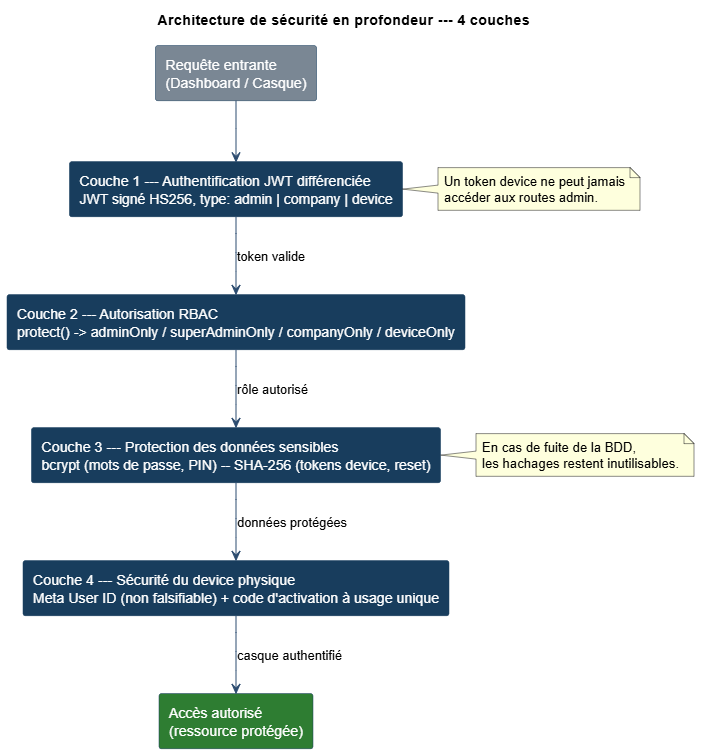
\includegraphics[width=0.85\textwidth]{../images/securite4couches.png}
  \caption{Architecture de sécurité en profondeur à quatre couches}
  \label{fig:securite}
\end{figure}

\subsubsection{Couche 1 --- Authentification JWT différenciée}

Le payload JWT encode le type d'acteur~: \texttt{\{id, type: 'admin'|'company'|'device', role?\}}.
Cette différenciation garantit qu'un token de type \texttt{device} ne peut jamais accéder
aux routes réservées aux admins, même en cas d'interception.

\begin{table}[H]
  \centering
  \begin{tabular}{lll}
    \toprule
    \textbf{Acteur} & \textbf{Type} & \textbf{Durée} \\
    \midrule
    Admin (superadmin / staff) & admin   & 7 jours \\
    Company (dashboard)        & company & 7 jours \\
    Device (casque Meta Quest~3) & device & 1 an \\
    \bottomrule
  \end{tabular}
  \caption{Tokens JWT par acteur}
  \label{tab:jwt_tokens}
\end{table}

Le token device a une durée d'un an car le casque est un device fixe appartenant à
l'entreprise (pas à l'employé individuel). Supprimer le token à chaque changement
d'employé forcerait une réactivation à chaque session, ce qui est opérationnellement
absurde.

\subsubsection{Couche 2 --- Autorisation RBAC}

Les middlewares Express forment une chaîne de contrôle d'accès~:

\begin{itemize}
  \item \texttt{protect()}~: vérifie et décode le JWT.
  \item \texttt{adminOnly()}~: vérifie \texttt{type === 'admin'}.
  \item \texttt{superAdminOnly()}~: vérifie \texttt{role === 'superadmin'}.
  \item \texttt{companyOnly()}~: vérifie \texttt{type === 'company'}.
  \item \texttt{deviceOnly()}~: vérifie \texttt{type === 'device'}.
\end{itemize}

\subsubsection{Couche 3 --- Protection des données sensibles}

\begin{itemize}
  \item \textbf{bcrypt 10 rounds}~: appliqué aux mots de passe Company/Admin et aux
    PINs des employés. 10 rounds $\approx$ 100~ms, délai intentionnel rendant les
    attaques brute force coûteuses en temps.
  \item \textbf{SHA-256 pour les tokens device}~: le token brut (plain) est exposé
    une seule fois, pendant 60 secondes. Seul son hash est stocké en base. En cas
    de compromission de la BDD, les tokens hachés sont inutilisables.
  \item \textbf{SHA-256 pour le reset password}~: même logique, avec expiration de
    30 min.
\end{itemize}

\subsubsection{Couche 4 --- Sécurité du device physique}

\begin{itemize}
  \item \textbf{Meta User ID}~: identifiant matériel unique fourni par le SDK Oculus,
    stable et impossible à falsifier (contrairement à \texttt{deviceUniqueIdentifier}
    qui peut changer après un factory reset).
  \item \textbf{Code d'activation}~: 6 chiffres aléatoires, expire après 15 minutes.
    Saisi manuellement par l'admin dans le dashboard.
\end{itemize}

\subsection{Cas d'utilisation --- Descriptions textuelles}

\begin{ucbox}{Activer un casque Meta Quest~3}
  \begin{tabular}{lp{9cm}}
    \textbf{Pré-conditions} & Casque physiquement présent, admin Staff connecté. \\
    \textbf{Acteur}         & Staff Admin Tynass. \\
    \textbf{Scénario}       &
      1. Unity envoie le Meta User ID à \texttt{POST /request-activation}. \newline
      2. Backend génère un code 6 chiffres aléatoire (expire 15 min). \newline
      3. Admin saisit le code dans la DevicesPage du dashboard. \newline
      4. Backend génère un JWT device (1 an) + stocke le hash SHA-256. \newline
      5. Unity appelle \texttt{POST /check} et reçoit le token brut (60~s). \newline
      6. Token stocké dans PlayerPrefs (permanent). \\
    \textbf{Exceptions}     & Code expiré (15 min) → admin régénère un nouveau code. \\
    \textbf{Post-conditions}& Casque actif en BDD, token persistant sur le casque. \\
  \end{tabular}
\end{ucbox}

\vspace{0.5cm}

\begin{ucbox}{Login employé via casque VR}
  \begin{tabular}{lp{9cm}}
    \textbf{Pré-conditions} & Casque activé, employee créé avec accessCode + PIN. \\
    \textbf{Acteur}         & Employé (via Meta Quest~3). \\
    \textbf{Scénario}       &
      1. Employé saisit son accessCode (format XX-001) via le panel. \newline
      2. Unity valide le format (Regex \texttt{\^{}[A-Z]\{2\}-\textbackslash d\{3\}\$}). \newline
      3. Employé saisit son PIN 4 chiffres via le numpad. \newline
      4. Unity envoie \texttt{POST /api/company/employees/login} avec
         \texttt{device\_token}. \newline
      5. Backend vérifie le PIN (\texttt{bcrypt.compare}) et retourne
         \texttt{employee + auth\_token}. \newline
      6. AppSession stocke les données employé. \\
    \textbf{Exceptions}     & Code invalide → message d'erreur. PIN incorrect → rejet. \\
    \textbf{Post-conditions}& Employé connecté, AppSession initialisée, ModulesPanel
                              chargé. \\
  \end{tabular}
\end{ucbox}

\vspace{0.5cm}

\begin{ucbox}{Soumettre une session de formation}
  \begin{tabular}{lp{9cm}}
    \textbf{Pré-conditions} & Simulation terminée, données collectées dans AppSession. \\
    \textbf{Acteur}         & Système Unity (automatique). \\
    \textbf{Scénario}       &
      1. \texttt{OnboardingManager} calcule le score final. \newline
      2. AppSession contient~: trainingId, employeeId, startedAt, score, criteria[]. \newline
      3. Unity appelle \texttt{POST /api/sessions/submit} (auth\_token dans le header). \newline
      4. Backend calcule \texttt{durationSeconds} (côté serveur, horloge fiable). \newline
      5. Backend incrémente \texttt{attemptNumber} via le pre-save hook. \newline
      6. Session stockée en BDD, visible dans le dashboard admin. \\
    \textbf{Exceptions}     & Perte Wi-Fi → retry automatique via TynassApiClient. \\
    \textbf{Post-conditions}& Session persistante, statistiques mises à jour. \\
  \end{tabular}
\end{ucbox}

\subsection{Diagrammes de séquence}

La figure~\ref{fig:seq_activation} illustre le déroulement complet de l'activation
d'un casque, depuis la demande initiale envoyée par l'application Unity jusqu'à la
récupération du jeton sécurisé.

\begin{figure}[H]
  \centering
  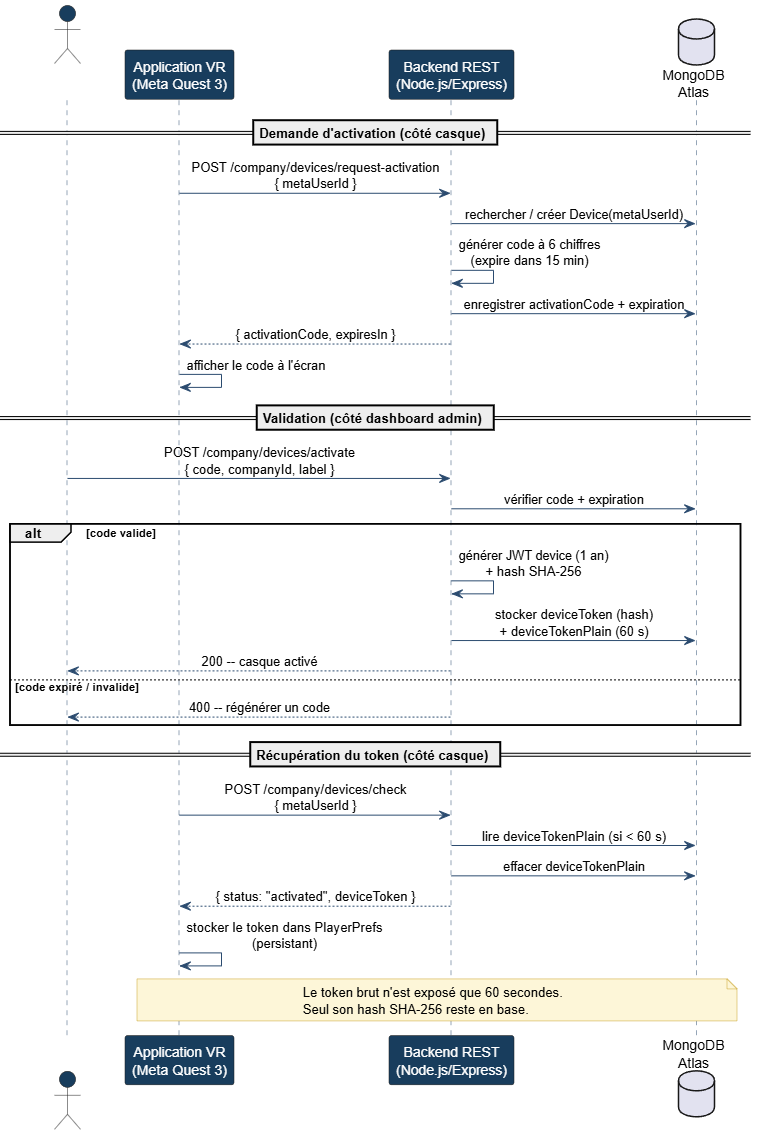
\includegraphics[width=0.9\textwidth]{../images/seqActivation.png}
  \caption{Diagramme de séquence --- activation d'un casque}
  \label{fig:seq_activation}
\end{figure}

\begin{figure}[H]
  \centering
  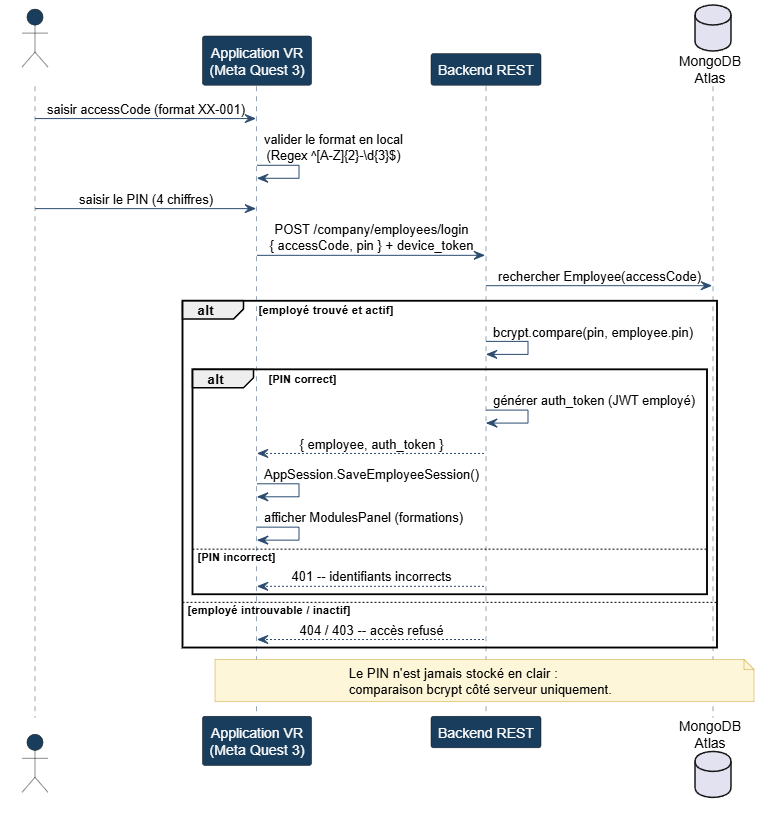
\includegraphics[width=0.9\textwidth]{../images/seqLogin.png}
  \caption{Diagramme de séquence --- login employé}
  \label{fig:seq_login}
\end{figure}

\section{Implémentation de l'itération~1}

Cette section détaille la mise en œuvre du backend~: la structure du projet selon le
patron MVC, les principales routes de l'API REST, et les fonctionnalités clés développées.

\subsection{Structure du projet --- Architecture MVC}

\placeholder{Arborescence des dossiers (à insérer)}

Le projet backend est organisé selon le pattern MVC~:

\begin{itemize}
  \item \texttt{models/}~: 8 schémas Mongoose (Company, Admin, Training, Session,
    Employee, Device, Counter, Quiz).
  \item \texttt{controllers/}~: logique métier séparée par domaine (admin.auth,
    company.auth, admin.companies, admin.trainings, session, employee, device).
  \item \texttt{routes/}~: points d'entrée REST groupés par acteur.
  \item \texttt{middleware/}~: \texttt{auth.middleware.js} avec les 5 guards.
  \item \texttt{utils/}~: \texttt{sendEmail.js} (Nodemailer).
\end{itemize}

\subsection{API REST --- Tableau des endpoints}

Le tableau~\ref{tab:endpoints} présente un extrait des routes principales de l'API.

\begin{table}[H]
  \centering
  \begin{tabularx}{\textwidth}{llXl}
    \toprule
    \textbf{Méthode} & \textbf{Route} & \textbf{Description} & \textbf{Auth} \\
    \midrule
    \multicolumn{4}{l}{\textit{Authentification Admin}} \\
    POST & \texttt{/api/admin/auth/setup} & Créer le 1er superadmin & Public \\
    POST & \texttt{/api/admin/auth/login} & Login admin & Public \\
    GET  & \texttt{/api/admin/auth/me} & Profil admin courant & Admin \\
    \midrule
    \multicolumn{4}{l}{\textit{Gestion Entreprises}} \\
    GET  & \texttt{/api/admin/companies} & Lister toutes les entreprises & Admin \\
    POST & \texttt{/api/admin/companies} & Créer une entreprise & Admin \\
    PATCH& \texttt{/api/admin/companies/:id} & Modifier une entreprise & Admin \\
    POST & \texttt{/api/admin/companies/:id/trainings} & Assigner une formation & Admin \\
    \midrule
    \multicolumn{4}{l}{\textit{Activation Casque}} \\
    POST & \texttt{/api/company/devices/request-activation} & Générer code 6 chiffres & Device \\
    POST & \texttt{/api/company/devices/activate} & Activer avec le code & Admin \\
    POST & \texttt{/api/company/devices/check} & Récupérer device token & Device \\
    \midrule
    \multicolumn{4}{l}{\textit{Login Employé}} \\
    POST & \texttt{/api/company/employees/login} & Login code + PIN & Device \\
    GET  & \texttt{/api/company/devices/trainings} & Formations du casque & Device \\
    \midrule
    \multicolumn{4}{l}{\textit{Sessions}} \\
    POST & \texttt{/api/sessions/submit} & Soumettre une session & Device \\
    GET  & \texttt{/api/sessions/stats} & Statistiques agrégées & Admin/Company \\
    \bottomrule
  \end{tabularx}
  \caption{Endpoints API --- extrait des routes principales}
  \label{tab:endpoints}
\end{table}

\subsection{Fonctionnalité clé --- Système d'activation du casque}

Le système d'activation est la fonctionnalité la plus originale du backend. Il repose
sur l'identifiant hardware Meta User ID, fourni par le SDK Oculus Platform et
impossible à falsifier. Le flow complet est le suivant~:

\begin{enumerate}
  \item L'application Unity envoie le Meta User ID au backend via
    \texttt{POST /request-activation}.
  \item Le backend génère un code aléatoire de 6 chiffres, le stocke haché (SHA-256)
    avec une expiration de 15 minutes, et retourne le code à l'affichage (pour l'admin).
  \item L'admin saisit ce code dans la DevicesPage du dashboard.
  \item Le backend vérifie le code, génère un JWT device (1 an), stocke le hash
    SHA-256 en BDD et expose le token brut pendant 60 secondes maximum.
  \item Unity appelle \texttt{POST /check}, récupère le token brut et le stocke
    dans PlayerPrefs. Le token brut est immédiatement effacé côté serveur.
\end{enumerate}

\subsection{Fonctionnalité clé --- Compteur atomique (accessCode)}

L'accessCode des employés suit le format XX-001 (2 lettres initiales de l'entreprise
+ numéro auto-incrémenté). Pour éviter les race conditions lors de créations
simultanées, le backend utilise la commande MongoDB
\texttt{findOneAndUpdate(\{key\}, \{\$inc: \{seq: 1\}\}, \{upsert: true, new: true\})},
garantissant une incrémentation atomique sans doublons.

\section{Difficultés et solutions}

\begin{table}[H]
  \centering
  \begin{tabularx}{\textwidth}{lXX}
    \toprule
    \textbf{Défi} & \textbf{Problème} & \textbf{Solution} \\
    \midrule
    Race condition & Deux employés créés simultanément pouvaient recevoir le même
                     accessCode (\texttt{countDocuments} non atomique). &
                     Migration vers Counter + \texttt{\$inc} MongoDB~: opération
                     atomique garantissant l'unicité. \\
    \midrule
    Sécurité token device & Stocker le device token en clair en BDD représentait
                            un risque en cas de compromission. &
                            SHA-256 permanent pour le stockage, token brut exposé
                            60~s uniquement puis effacé. \\
    \midrule
    UnityWebRequest 4xx & Unity traitait les réponses HTTP 4xx comme des erreurs
                          réseau sans lire le body JSON. &
                          Restructuration des réponses backend~: toujours
                          retourner un body JSON lisible même sur les erreurs. \\
    \midrule
    Pre-save hook & Utiliser \texttt{async function(next)} dans un hook
                    Mongoose async causait l'erreur
                    \og~next is not a function~\fg. &
                    Suppression du paramètre \texttt{next}~: en Mongoose,
                    les hooks async gèrent automatiquement la promesse. \\
    \bottomrule
  \end{tabularx}
  \caption{Difficultés rencontrées et solutions --- Itération~1}
  \label{tab:dificultes_s1}
\end{table}

\section{Évaluation de l'itération~1}

\begin{table}[H]
  \centering
  \begin{tabularx}{\textwidth}{Xl}
    \toprule
    \textbf{Élément validé} & \textbf{Statut} \\
    \midrule
    Authentification différenciée des trois acteurs (Admin, Company, Device) & Fonctionnel \\
    Activation d'un casque via code à 6 chiffres + jeton haché SHA-256 & Fonctionnel \\
    Login employé (code d'accès + PIN) & Fonctionnel \\
    Enregistrement et restitution des sessions de formation & Fonctionnel \\
    Agrégation des statistiques par formation et par entreprise & Fonctionnel \\
    Tests des endpoints via Postman & Validé \\
    \bottomrule
  \end{tabularx}
  \caption{Validation fonctionnelle --- Itération~1}
  \label{tab:eval_s1}
\end{table}

\placeholder{Capture Postman --- Réponse POST /api/company/devices/check (à insérer)}

\placeholder{Capture MongoDB Compass --- Collections créées (à insérer)}

\section{Conclusion}

Cette première itération a livré le backend complet de \tynassit{}, déployé sur Render
(\texttt{tynassit-backend-pfe.onrender.com}). L'architecture de sécurité à 4 couches
garantit l'isolation des acteurs et la protection des données sensibles. Le système
d'activation des casques, combinant identifiant matériel Meta User ID et code
d'activation à usage unique, constitue la fonctionnalité la plus originale du projet.

% ================================================================
% chapters/chapter4.tex --- RECONSTRUCTION (même structure que ch.3)
% ----------------------------------------------------------------
% Backlog restructuré~: Titre + Charge (j/h) ajoutées, Statut retiré
% + phrase de synthèse. Charge (j/h) = MES ESTIMATIONS RELATIVES,
% pas des mesures réelles --- à remplacer si tu as de vraies données.
% Rien d'autre n'est modifié dans ce chapitre.
% ================================================================

\chapter{Itération~2 --- Dashboards Web Admin et Company}

\section{Introduction}

Cette itération couvre le développement des deux interfaces web de \tynassit{}~:
le \textbf{dashboard Admin} destiné aux équipes Tynass, et le \textbf{dashboard Company}
destiné aux entreprises clientes. Les deux dashboards sont développés avec React,
TypeScript et déployés séparément sur Vercel pour garantir une isolation totale.

\section{Planification de l'itération~2}

\subsection{Objectifs}

\begin{itemize}
  \item Livrer 7 pages fonctionnelles pour le dashboard Admin.
  \item Livrer 6 pages fonctionnelles pour le dashboard Company.
  \item Connecter les deux dashboards au backend via l'API REST.
  \item Déployer les deux dashboards en production sur Vercel.
\end{itemize}

\subsection{Tâches et estimations de l'itération~2}

\begin{table}[H]
  \centering
  \small
  \setlength{\tabcolsep}{5pt}
  \begin{tabularx}{\textwidth}{cp{3.5cm}Xc>{\footnotesize}c}
    \toprule
    \textbf{ID} & \textbf{Titre} & \textbf{Tâches principales} & \textbf{MoSCoW} & \textbf{Charge estimée (j/h)} \\
    \midrule
    US-06 & Connexion Admin &
      LoginPage admin + AuthProvider + JWT localStorage & \must{} & 1,5 \\
    US-07 & KPIs du dashboard &
      DashboardPage --- 4 KPIs + Top 5 Companies/Trainings & \must{} & 2 \\
    US-08 & Gestion des entreprises &
      CompaniesPage --- CRUD + toggle + assign formations & \must{} & 2,5 \\
    US-09 & Gestion des casques &
      DevicesPage --- activation (code 6 chiffres) + révocation & \must{} & 2 \\
    US-10 & Filtrage des sessions &
      SessionsPage --- filtres company/training/date & \should{} & 1,5 \\
    US-11 & Connexion Company &
      LoginPage company + AuthProvider company & \must{} & 1 \\
    US-12 & Gestion des employés &
      EmployeesPage --- CRUD + accessCode + PIN & \must{} & 2 \\
    US-13 & Historique Company &
      SessionsPage company --- historique + pagination & \should{} & 1,5 \\
    \midrule
    \multicolumn{4}{r}{\textbf{Total estimé}} & \textbf{14} \\
    \bottomrule
  \end{tabularx}
  \caption{Tâches et estimations --- Itération~2}
  \label{tab:backlog_s2}
\end{table}

\noindent Toutes les user stories de cette itération ont été livrées.

\section{Conception de l'itération~2}

Cette section présente les choix technologiques retenus pour les deux dashboards web
ainsi que le système d'authentification mis en place.

\subsection{Décisions architecturales --- Frontend}

\begin{table}[H]
  \centering
  \begin{tabularx}{\textwidth}{lllX}
    \toprule
    \textbf{Composant} & \textbf{Retenu} & \textbf{Alternative} & \textbf{Justification} \\
    \midrule
    Framework  & React + TS  & Vue, Angular   & Maîtrise préalable, écosystème npm,
                                                typage strict \\
    Language   & TypeScript  & JavaScript     & Détection erreurs à la compilation,
                                                interfaces pour types API \\
    Bundler    & Vite        & CRA, Webpack   & Démarrage instantané (ESM natif),
                                                HMR ultra-rapide \\
    Router     & React Router v6 & TanStack Start & SSR bloquait les appels fetch API
                                                    côté client \\
    Data       & TanStack Query & SWR, Axios  & Cache automatique, invalidation après
                                                mutation, états loading/error natifs \\
    UI         & Shadcn UI   & Material UI    & Composants copiés dans le projet
                                                (pas de lock-in), basés sur Radix UI \\
    CSS        & Tailwind v3 & Tailwind v4    & Incompatibilité v4 avec composants
                                                Shadcn UI \\
    Animations & Framer Motion & CSS seul    & Transitions fluides, animations déclaratives \\
    Toasts     & Sonner      & React-Toastify & API simple, design moderne \\
    Déploiement & Vercel     & Netlify        & CI/CD automatique depuis GitHub \\
    \bottomrule
  \end{tabularx}
  \caption{Décisions architecturales --- Dashboards React}
  \label{tab:archi_frontend}
\end{table}

\subsection{Pourquoi deux projets séparés~?}

Un seul projet avec gestion des rôles aurait été possible, mais deux projets séparés
ont été préférés pour les raisons suivantes~:

\begin{itemize}
  \item \textbf{Isolation totale des données}~: le dashboard Company n'a accès qu'aux
    routes \texttt{/api/company/*}, jamais aux routes admin.
  \item \textbf{Déploiements indépendants}~: une mise à jour du dashboard Admin
    n'affecte pas le dashboard Company.
\end{itemize}

\subsection{Système d'authentification}

L'authentification aux dashboards repose sur un jeton JWT. La figure~\ref{fig:seq_login_admin}
présente la séquence de connexion d'un administrateur, depuis la saisie de ses identifiants
jusqu'à la validation du jeton et le chargement de son profil.

\begin{figure}[H]
  \centering
  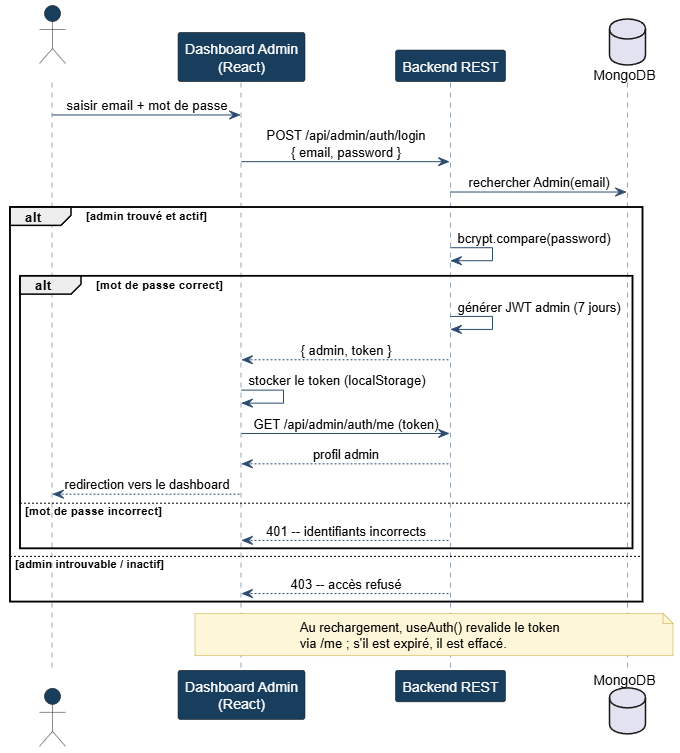
\includegraphics[width=0.9\textwidth]{../images/seqLoginAdmin.png}
  \caption{Diagramme de séquence --- login administrateur}
  \label{fig:seq_login_admin}
\end{figure}

Le JWT admin est stocké dans \texttt{localStorage("admin\_token")}. Au chargement de
l'application, le hook \texttt{useAuth()} appelle \texttt{api.getMe()} pour valider
le token et récupérer le profil admin. Si le token est expiré, \texttt{.catch()}
l'efface automatiquement et redirige vers la page de connexion.

\subsection{Cas d'utilisation --- Descriptions textuelles}

\begin{ucbox}{Activer un casque (côté Dashboard)}
  \begin{tabular}{lp{9cm}}
    \textbf{Pré-conditions} & Admin connecté, casque affichant un code 6 chiffres. \\
    \textbf{Acteur}         & Staff Admin Tynass. \\
    \textbf{Scénario}       &
      1. Admin ouvre DevicesPage et clique « Activate Device ». \newline
      2. Admin saisit le code 6 chiffres affiché sur le casque. \newline
      3. Admin sélectionne l'entreprise propriétaire du casque. \newline
      4. Admin saisit un label optionnel (ex~: « Salle de formation A »). \newline
      5. Dashboard appelle \texttt{POST /api/company/devices/activate}. \newline
      6. Succès~: le casque apparaît dans la liste comme « Active ». \\
    \textbf{Exceptions}     & Code expiré (15 min) → message d'erreur, régénérer. \\
    \textbf{Post-conditions}& Casque actif, apparaît dans la liste des devices. \\
  \end{tabular}
\end{ucbox}

\vspace{0.5cm}

\begin{ucbox}{Créer un employé avec accessCode et PIN}
  \begin{tabular}{lp{9cm}}
    \textbf{Pré-conditions} & Manager Company connecté au dashboard. \\
    \textbf{Acteur}         & Company (client B2B). \\
    \textbf{Scénario}       &
      1. Manager ouvre EmployeesPage et clique « Créer employé ». \newline
      2. Saisie~: nom, prénom, poste, département. \newline
      3. Saisie du PIN 4 chiffres (haché bcrypt côté backend). \newline
      4. Dashboard appelle \texttt{POST /api/company/employees}. \newline
      5. Backend génère l'accessCode (ex~: IN-001) via Counter + \texttt{\$inc}. \newline
      6. L'accessCode est affiché en lecture seule dans la fiche employé. \\
    \textbf{Post-conditions}& Employé créé, accessCode communiqué à l'employé. \\
  \end{tabular}
\end{ucbox}

\section{Implémentation de l'itération~2}

Cette section détaille les pages développées pour chacun des deux dashboards, en
commençant par le dashboard Admin destiné aux équipes Tynass, puis le dashboard Company
destiné aux entreprises clientes.

\subsection{Dashboard Admin --- Pages implémentées}

Le dashboard Admin regroupe sept pages, décrites ci-dessous.

\subsubsection{LoginPage}

Interface d'authentification avec animation Framer Motion (fade-in + scale de la
carte). Le formulaire appelle \texttt{POST /api/admin/auth/login} et stocke le JWT
dans \texttt{localStorage}.

\begin{figure}[H]
  \centering
  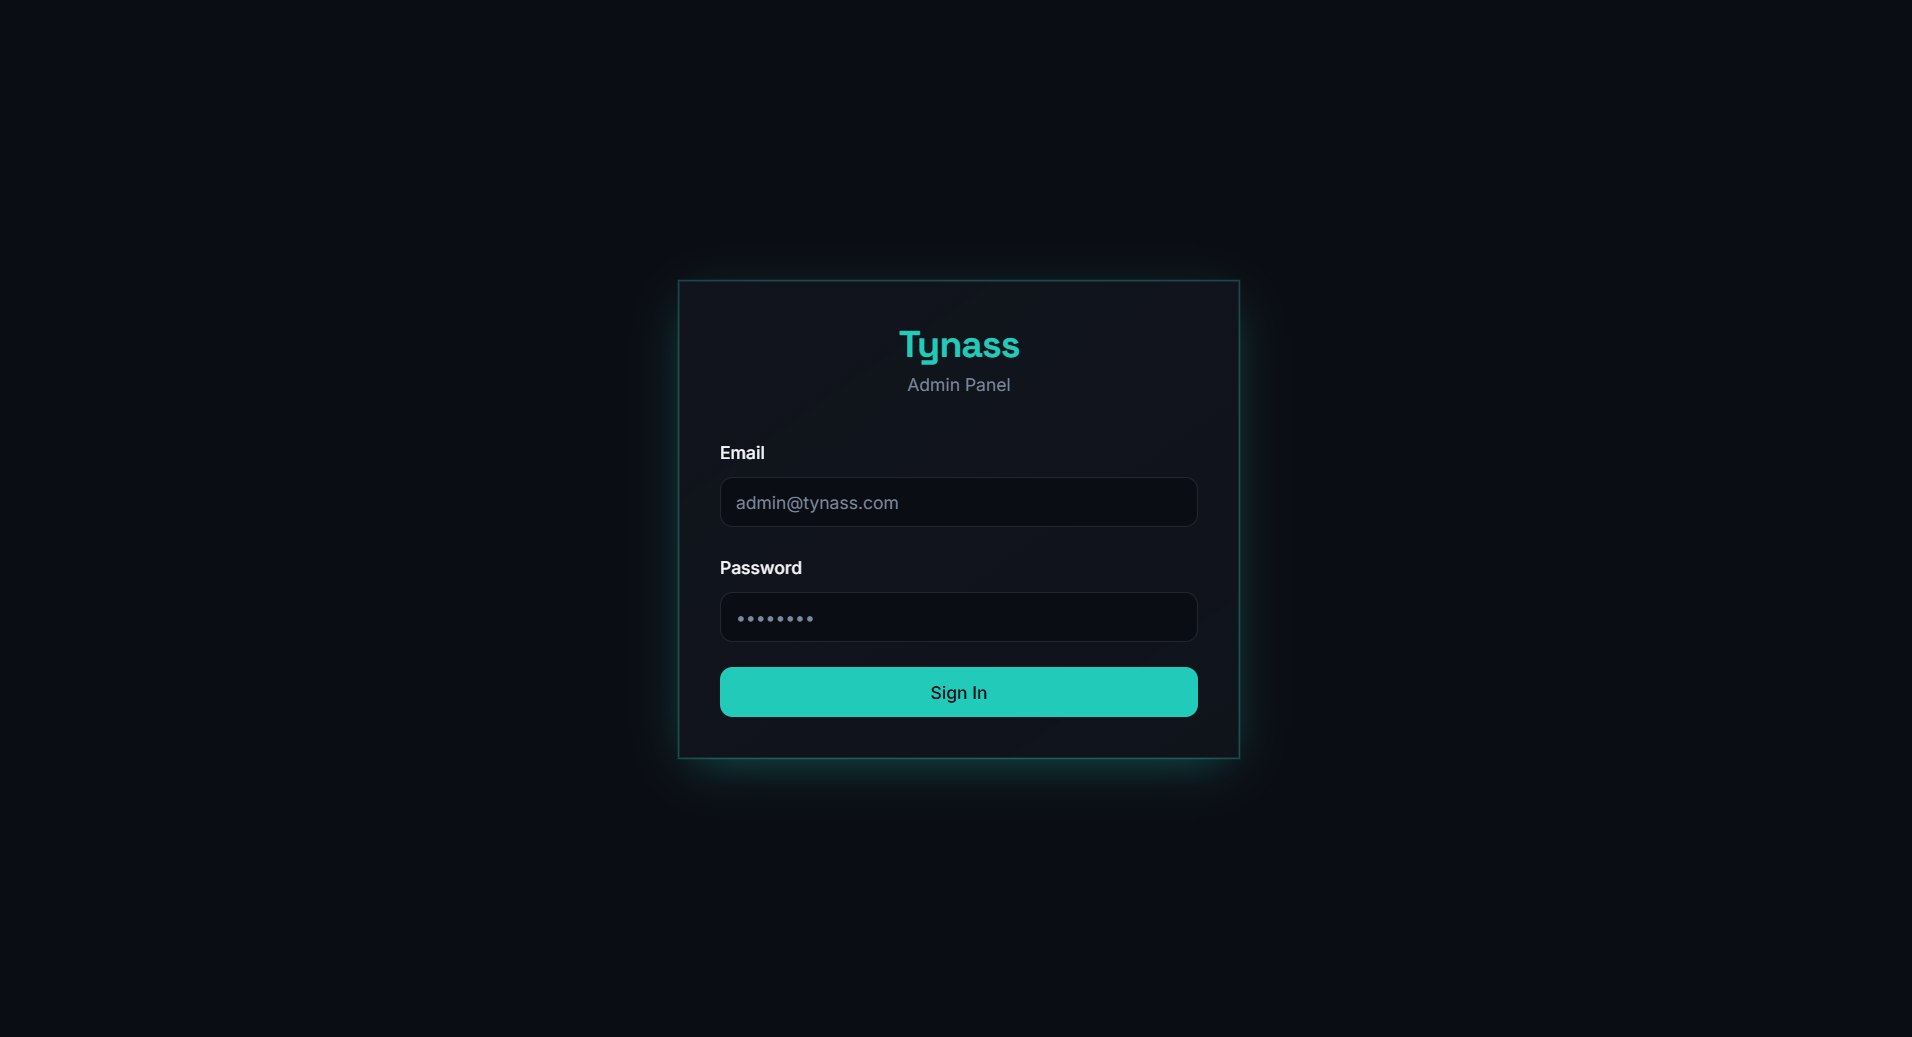
\includegraphics[width=0.8\textwidth]{../images/dashAdmin_login.png}
  \caption{Dashboard Admin --- page de connexion}
  \label{fig:dash_admin_login}
\end{figure}

\subsubsection{DashboardPage}

Page d'accueil affichant 4 KPIs calculés depuis le backend~: Total Companies, Total
Trainings, Sessions Played, Global Pass Rate. Affiche également les 5 entreprises
les plus actives et les 5 formations les plus jouées.

\begin{figure}[H]
  \centering
  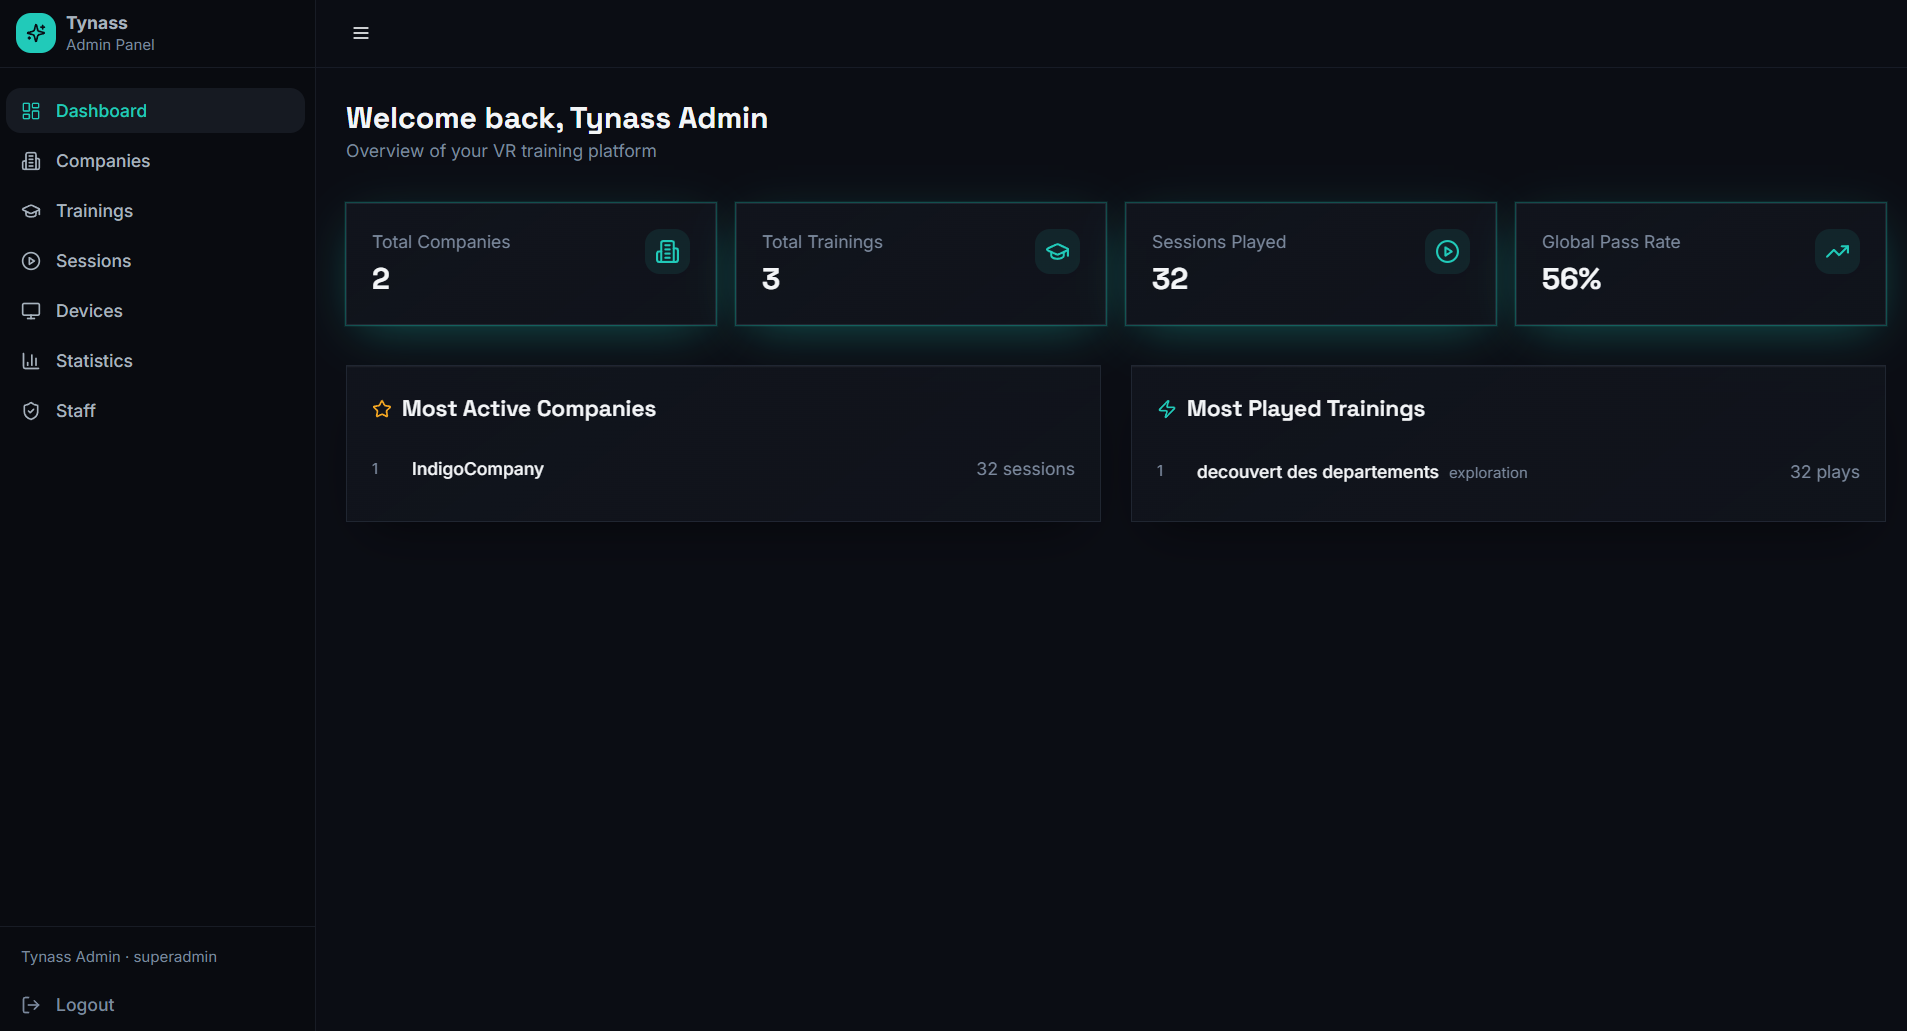
\includegraphics[width=\textwidth]{../images/dashAdmin_kpis.png}
  \caption{Dashboard Admin --- indicateurs clés (KPIs)}
  \label{fig:dash_admin_kpis}
\end{figure}

\subsubsection{CompaniesPage}

Gestion complète des entreprises clientes~: création, modification, suppression
(superadmin uniquement), activation/désactivation, et assignation des formations
via un dialog interactif.

\begin{figure}[H]
  \centering
  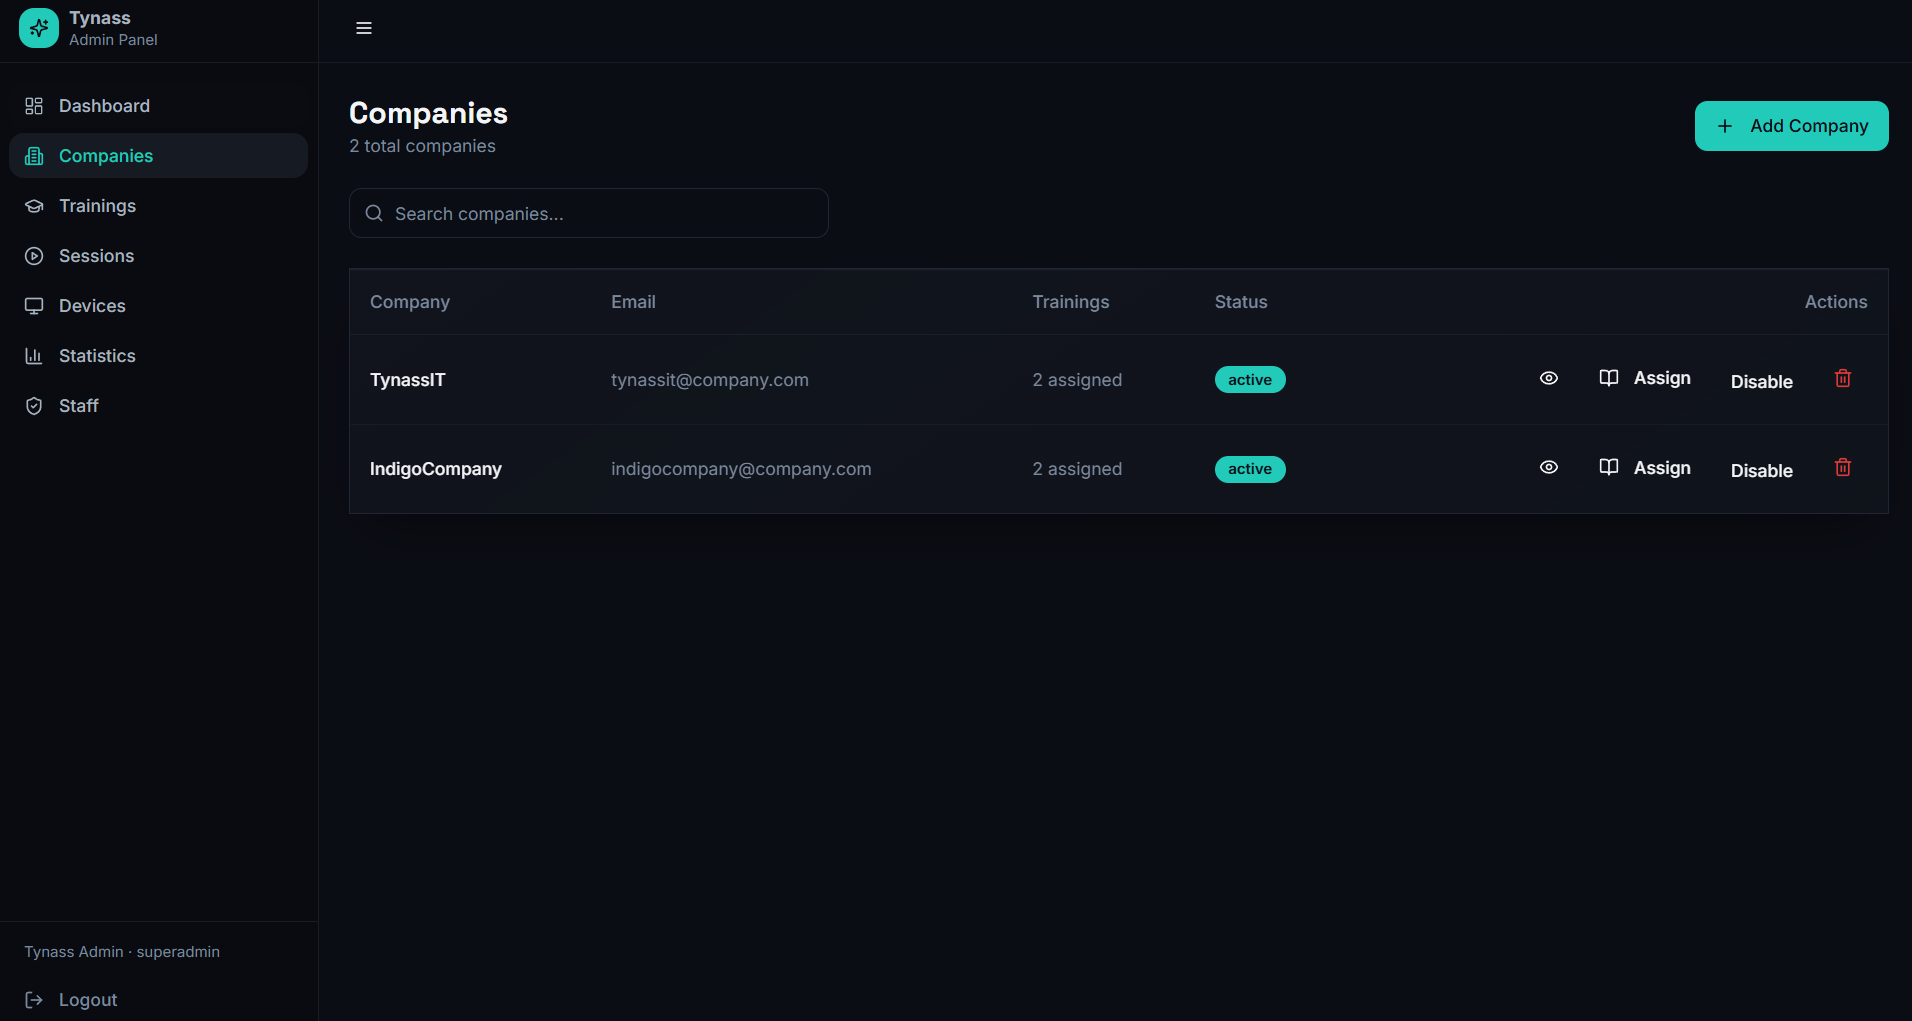
\includegraphics[width=\textwidth]{../images/dashAdmin_companies.png}
  \caption{Dashboard Admin --- gestion des entreprises}
  \label{fig:dash_admin_companies}
\end{figure}

\subsubsection{TrainingsPage}

Gestion du catalogue de formations VR. Le champ \texttt{sceneName} est crucial~: il
correspond exactement au nom de la scène Unity à charger via
\texttt{SceneManager.LoadScene(training.sceneName)}.

\begin{figure}[H]
  \centering
  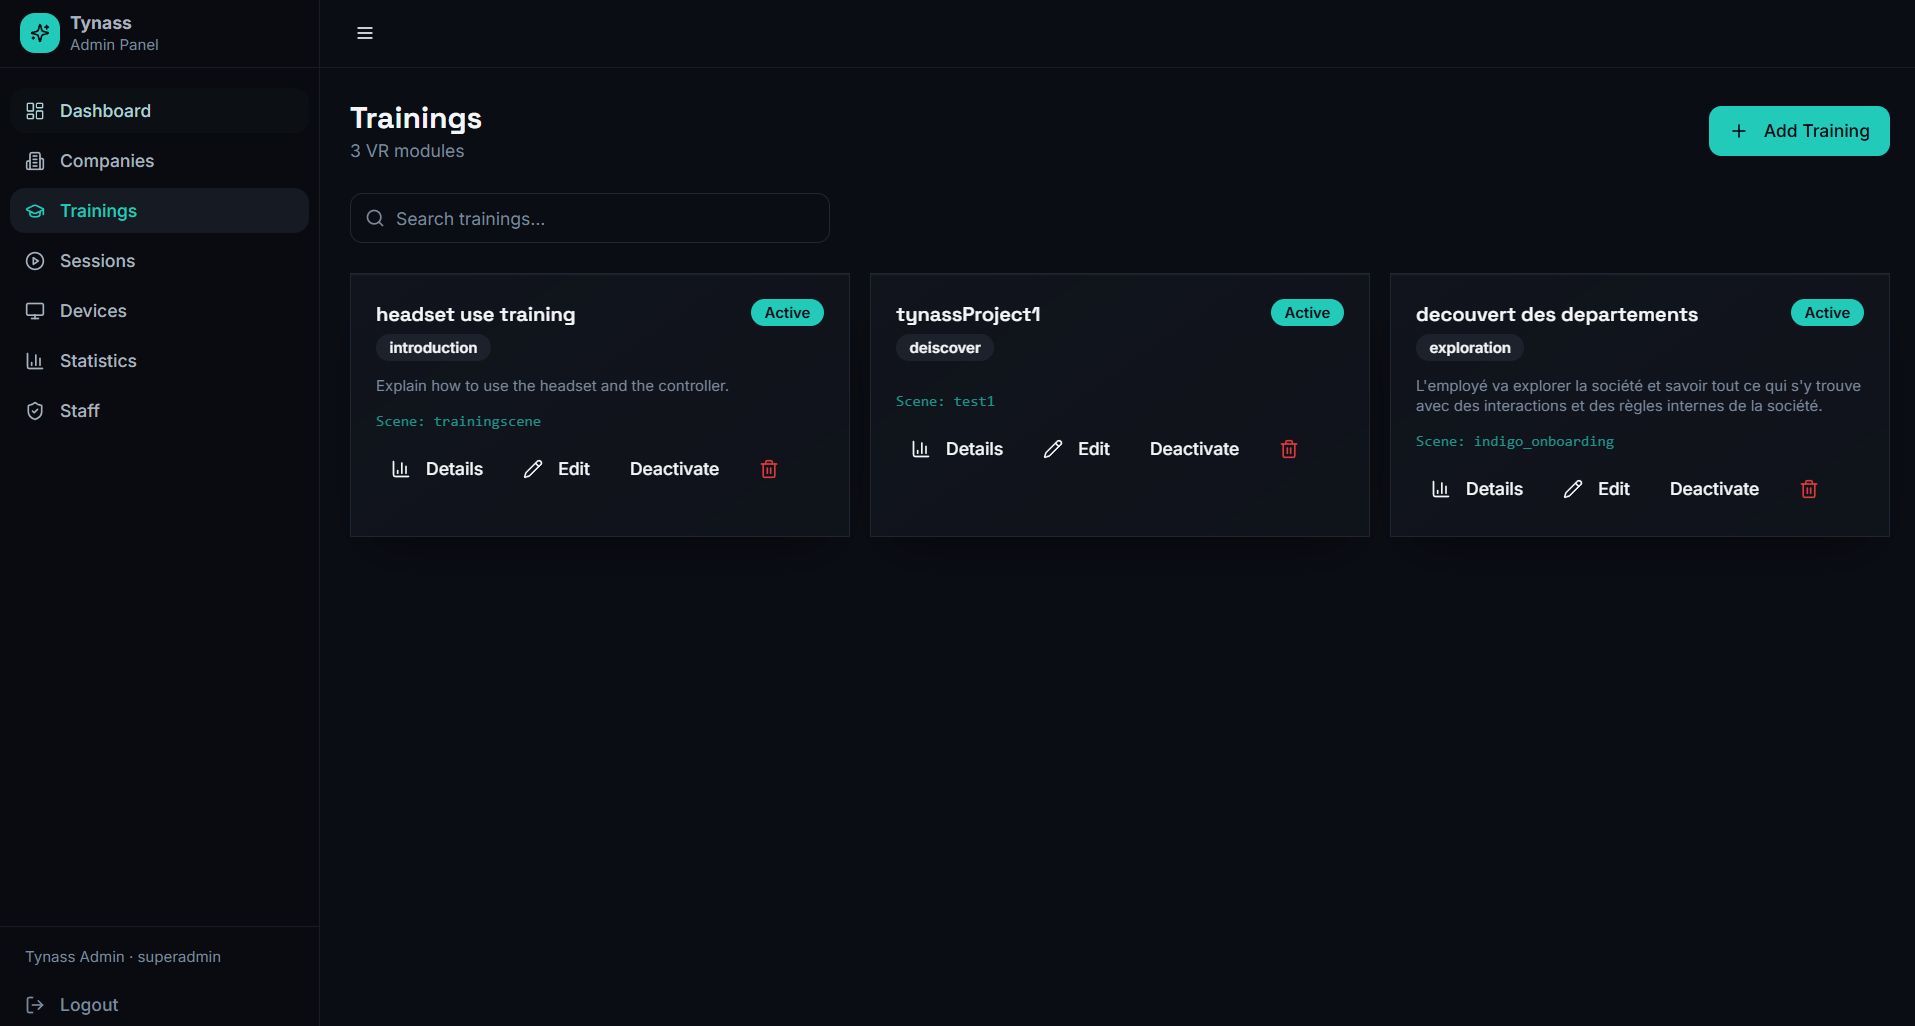
\includegraphics[width=\textwidth]{../images/dashAdmin_trainings.png}
  \caption{Dashboard Admin --- catalogue de formations et champ \texttt{sceneName}}
  \label{fig:dash_admin_trainings}
\end{figure}

\subsubsection{DevicesPage}

Activation et révocation des casques Meta Quest~3. L'admin saisit le code 6 chiffres
affiché sur le casque, sélectionne l'entreprise et confirme l'activation.

\begin{figure}[H]
  \centering
  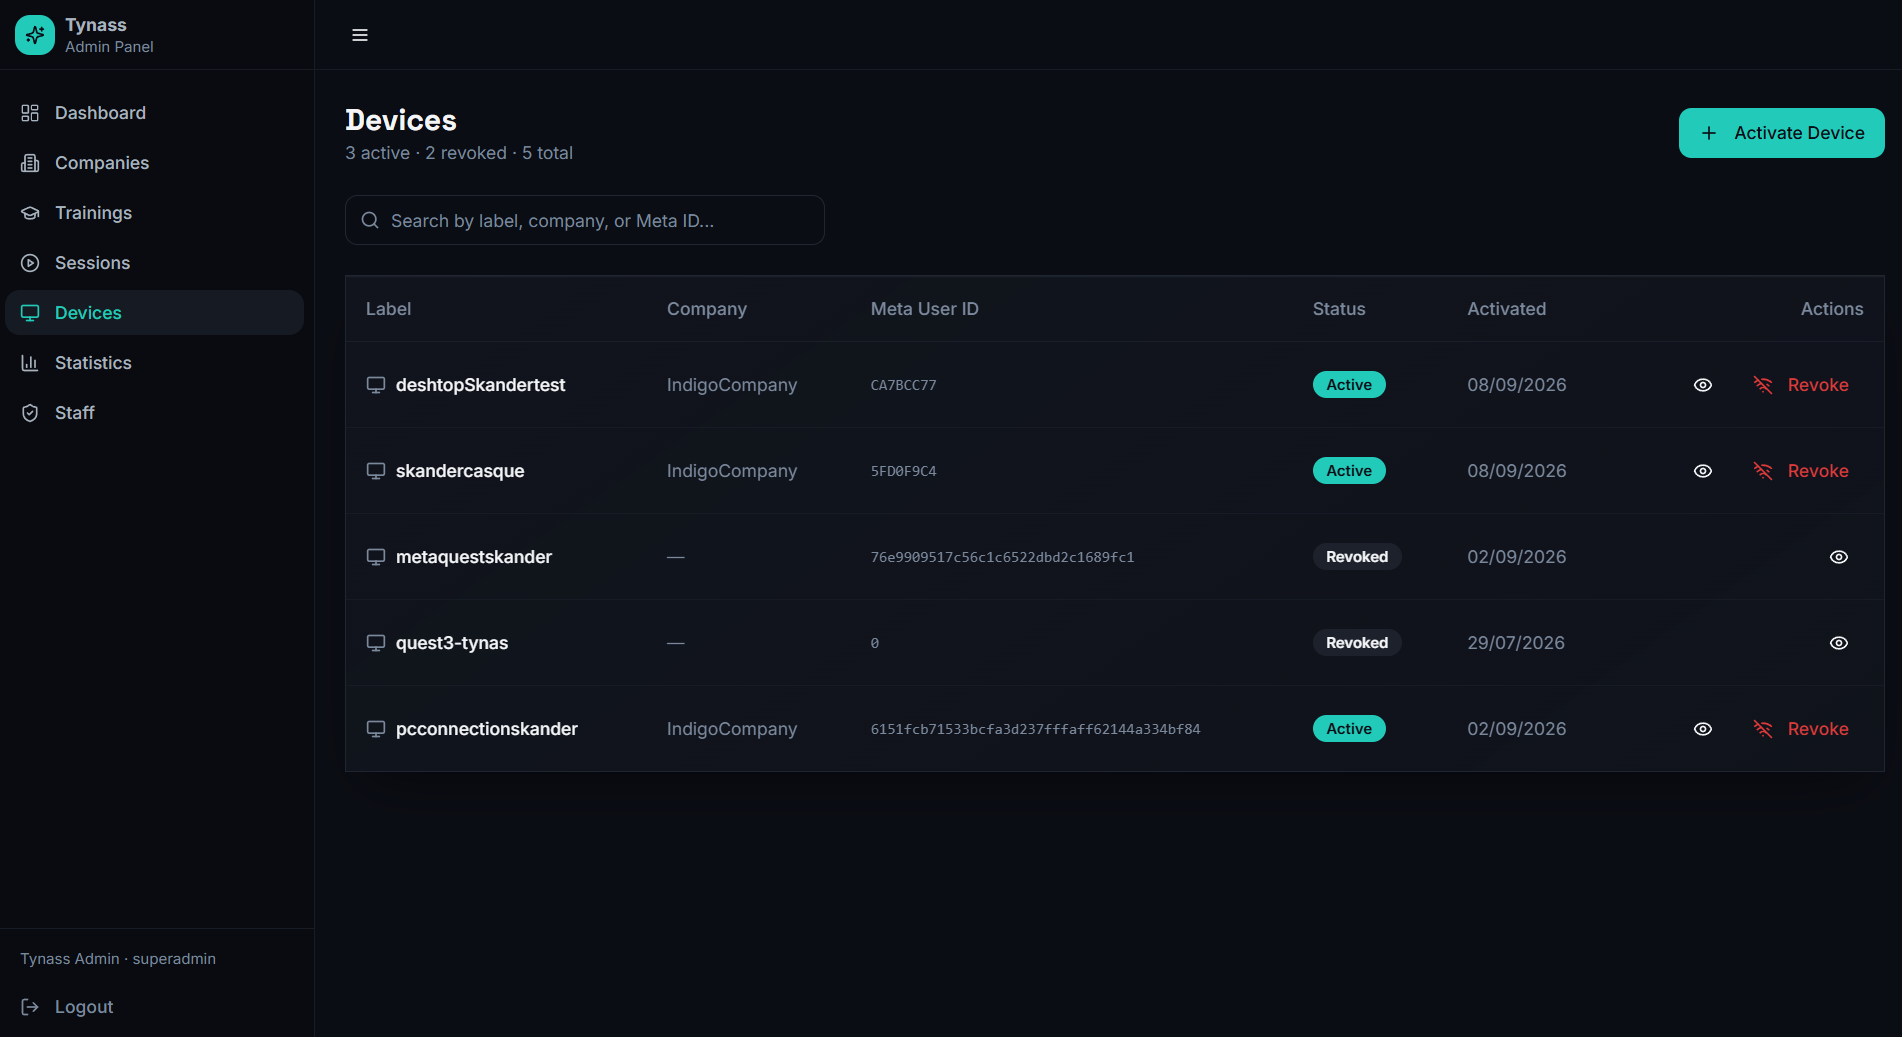
\includegraphics[width=\textwidth]{../images/dashAdmin_devices.png}
  \caption{Dashboard Admin --- activation d'un casque}
  \label{fig:dash_admin_devices}
\end{figure}

\subsubsection{SessionsPage}

Historique de toutes les sessions avec filtres multi-critères~: \texttt{companyFilter},
\texttt{trainingFilter}, \texttt{dateFrom}, \texttt{dateTo}. Le filtrage est effectué
côté client (JavaScript) sur le tableau complet retourné par l'API.

\begin{figure}[H]
  \centering
  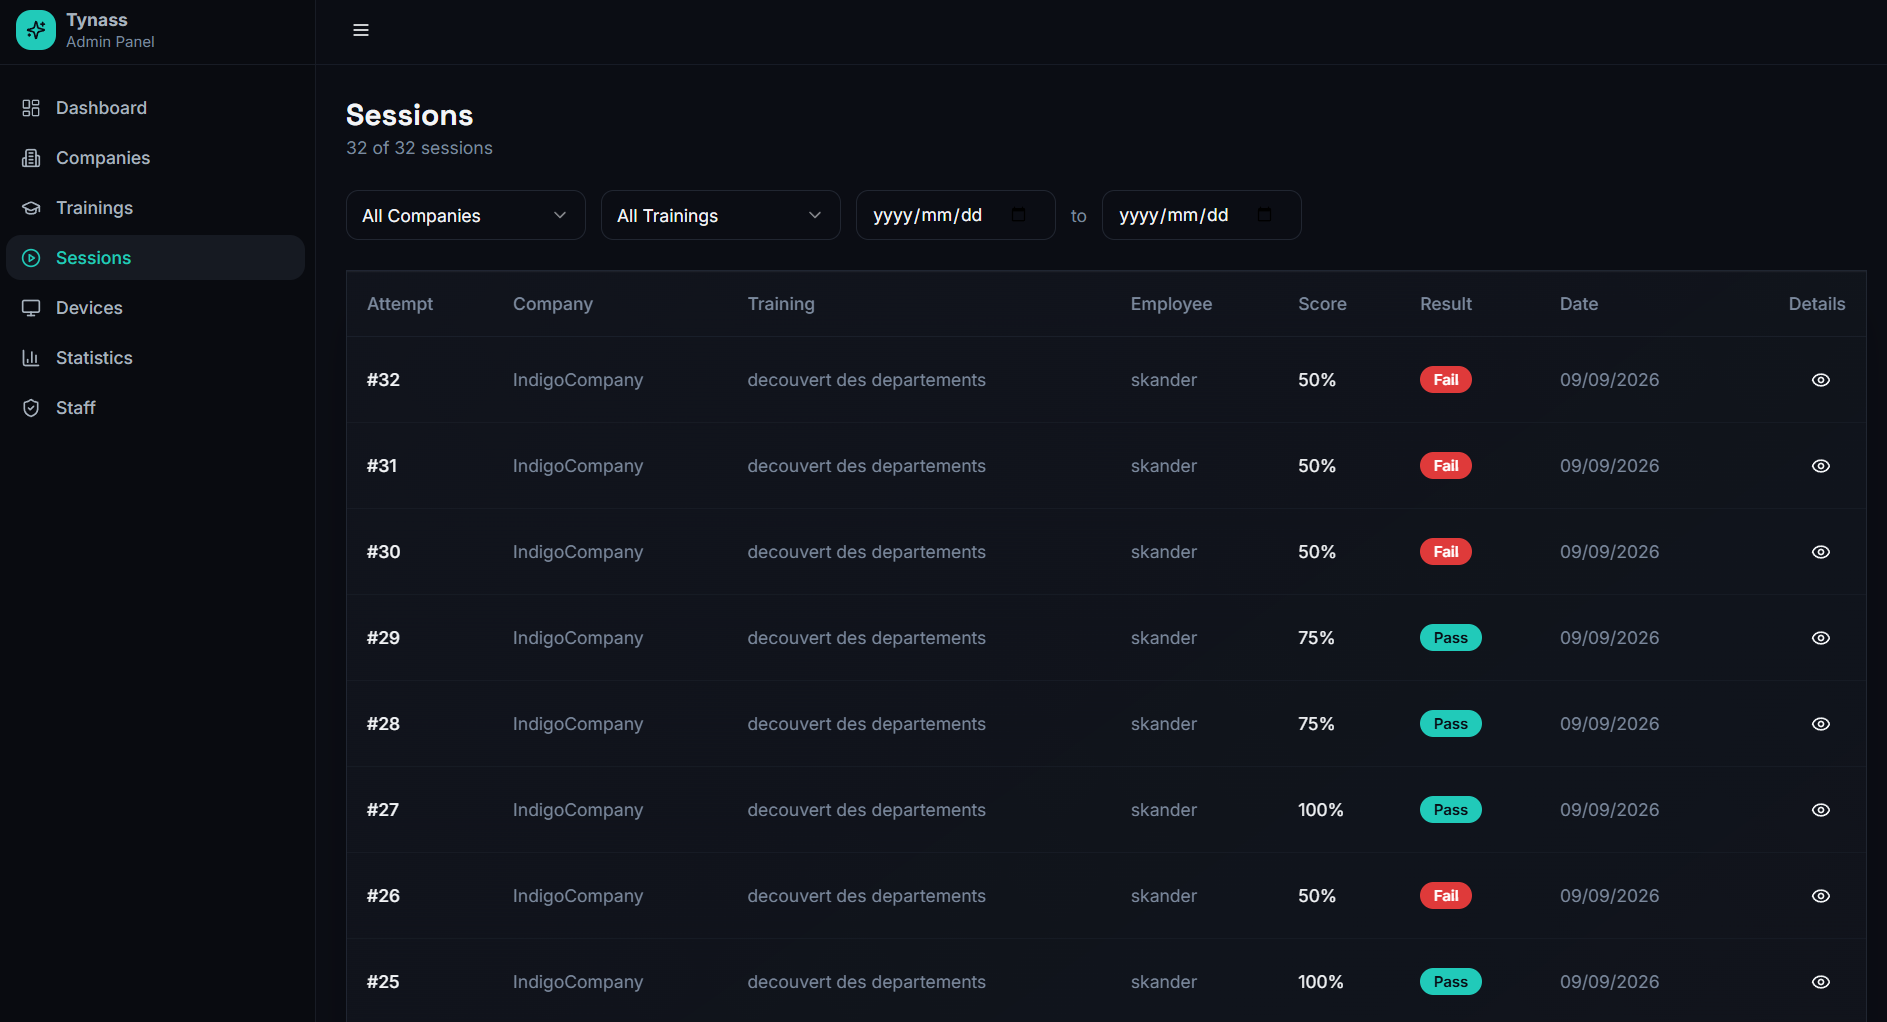
\includegraphics[width=\textwidth]{../images/dashAdmin_sessions.png}
  \caption{Dashboard Admin --- historique des sessions et filtres}
  \label{fig:dash_admin_sessions}
\end{figure}

\subsubsection{StatisticsPage}

Visualisation des statistiques agrégées par formation et par entreprise, calculées
via les pipelines d'agrégation MongoDB.

\begin{figure}[H]
  \centering
  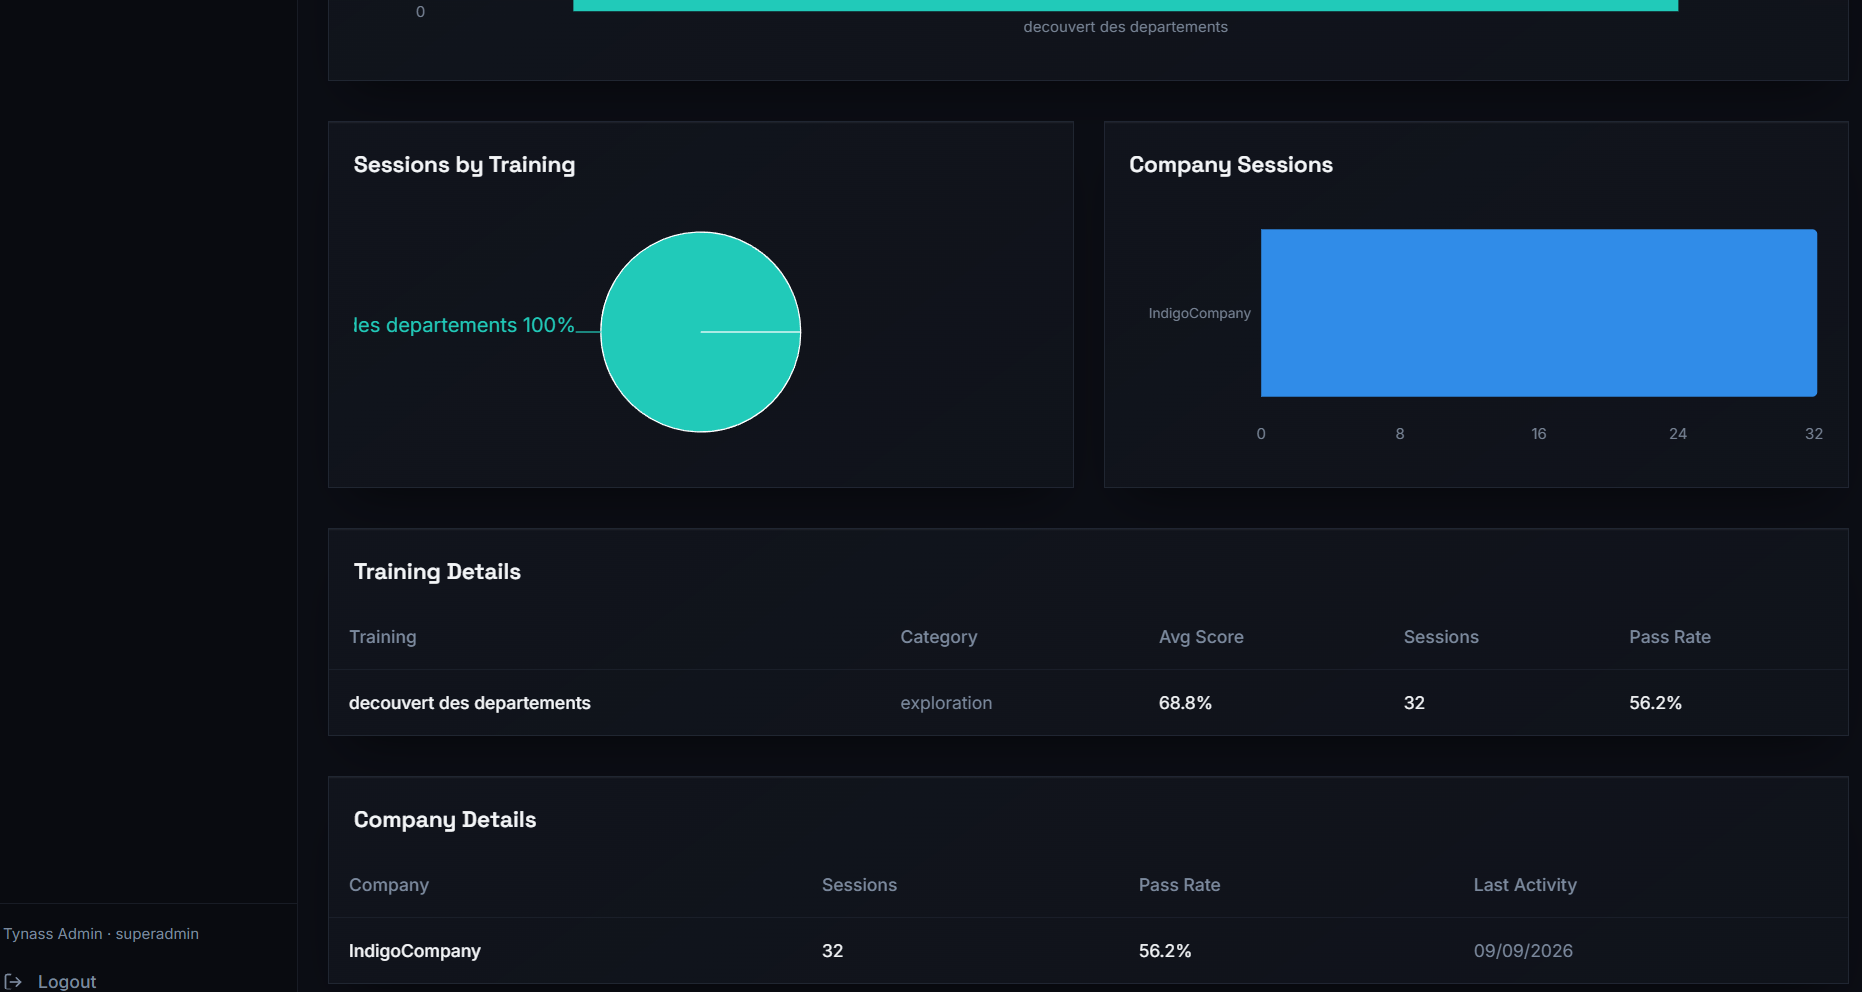
\includegraphics[width=\textwidth]{../images/dashAdmin_stats.png}
  \caption{Dashboard Admin --- statistiques agrégées}
  \label{fig:dash_admin_stats}
\end{figure}

\subsection{Dashboard Company --- Pages implémentées}

Le dashboard Company regroupe les pages permettant à l'entreprise de gérer ses employés
et de suivre leurs sessions.

\subsubsection{EmployeesPage}

Page centrale du dashboard Company~: CRUD complet des employés, affichage de
l'accessCode (lecture seule après création), saisie du PIN lors de la création, et
consultation des milestones de chaque employé.

\begin{figure}[H]
  \centering
  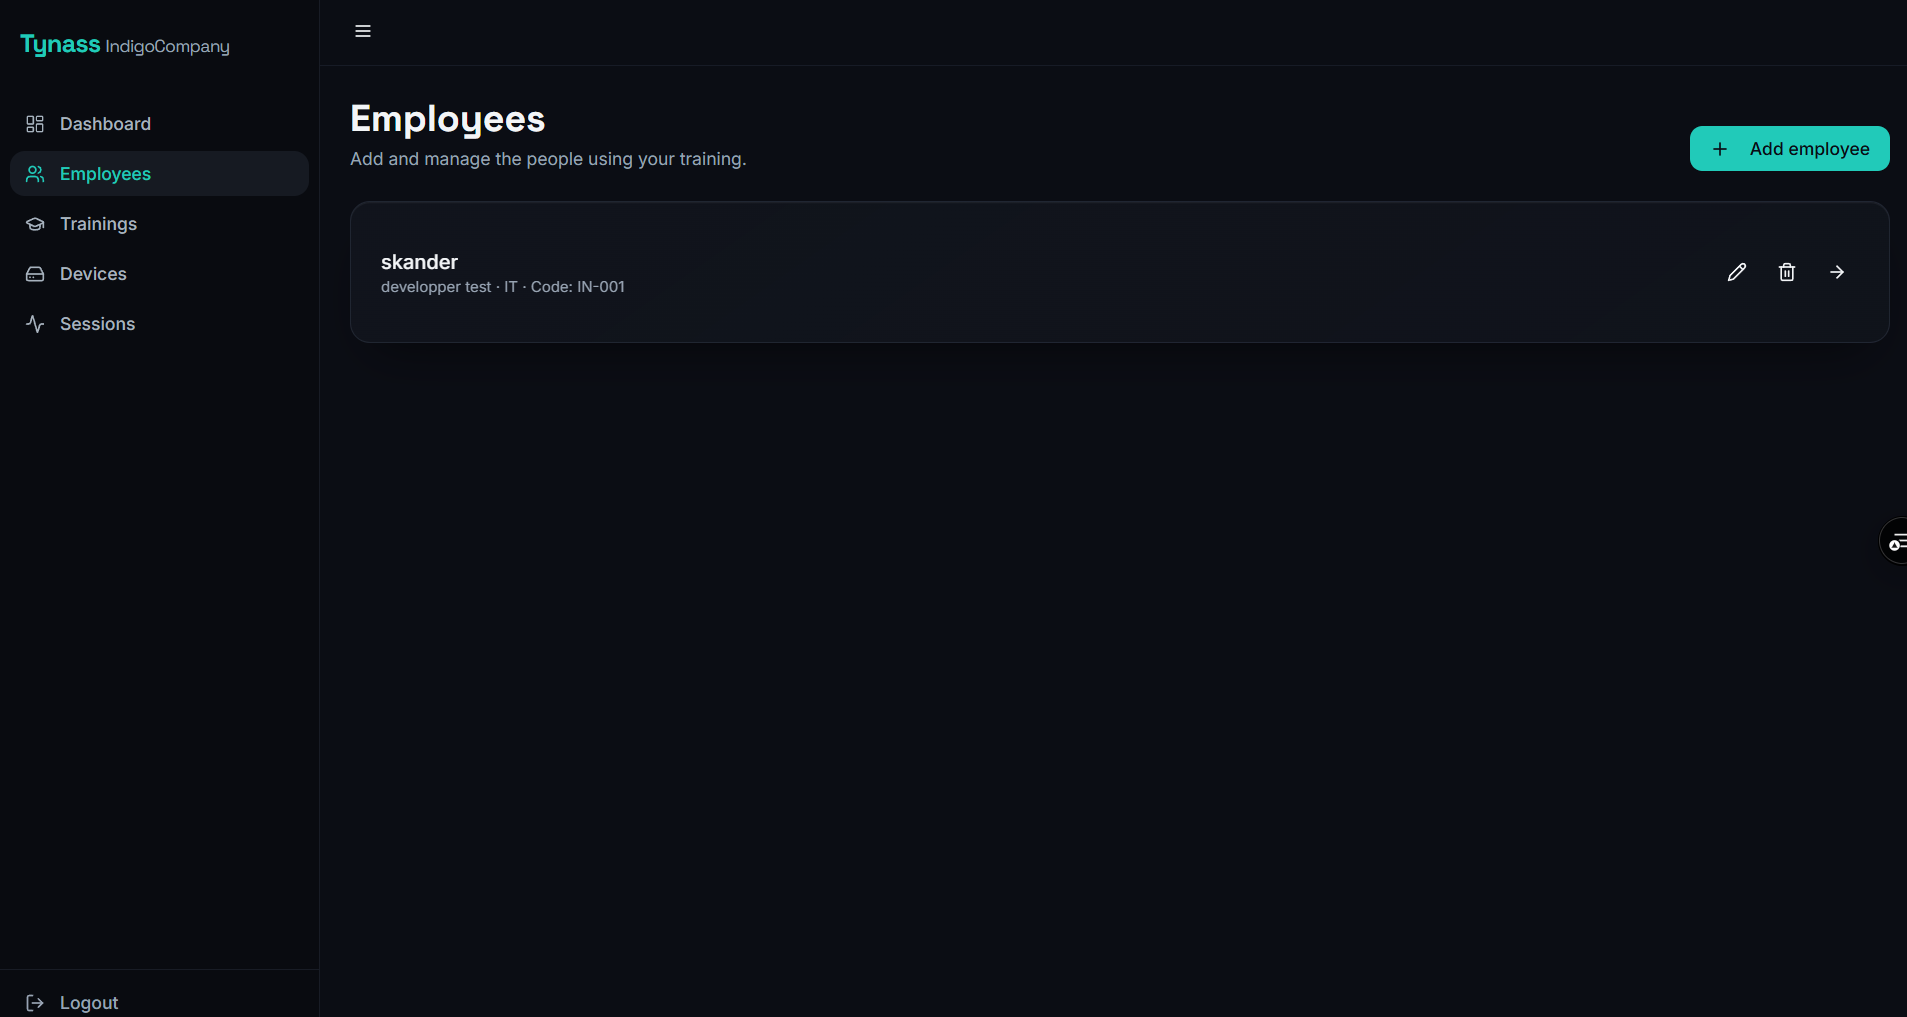
\includegraphics[width=\textwidth]{../images/dashCompany_employees.png}
  \caption{Dashboard Company --- gestion des employés}
  \label{fig:dash_company_employees}
\end{figure}

\subsubsection{SessionsPage Company}

Historique des sessions avec pagination frontend (PAGE\_SIZE = 20 sessions par page),
filtrage par employé ou par formation.

\begin{figure}[H]
  \centering
  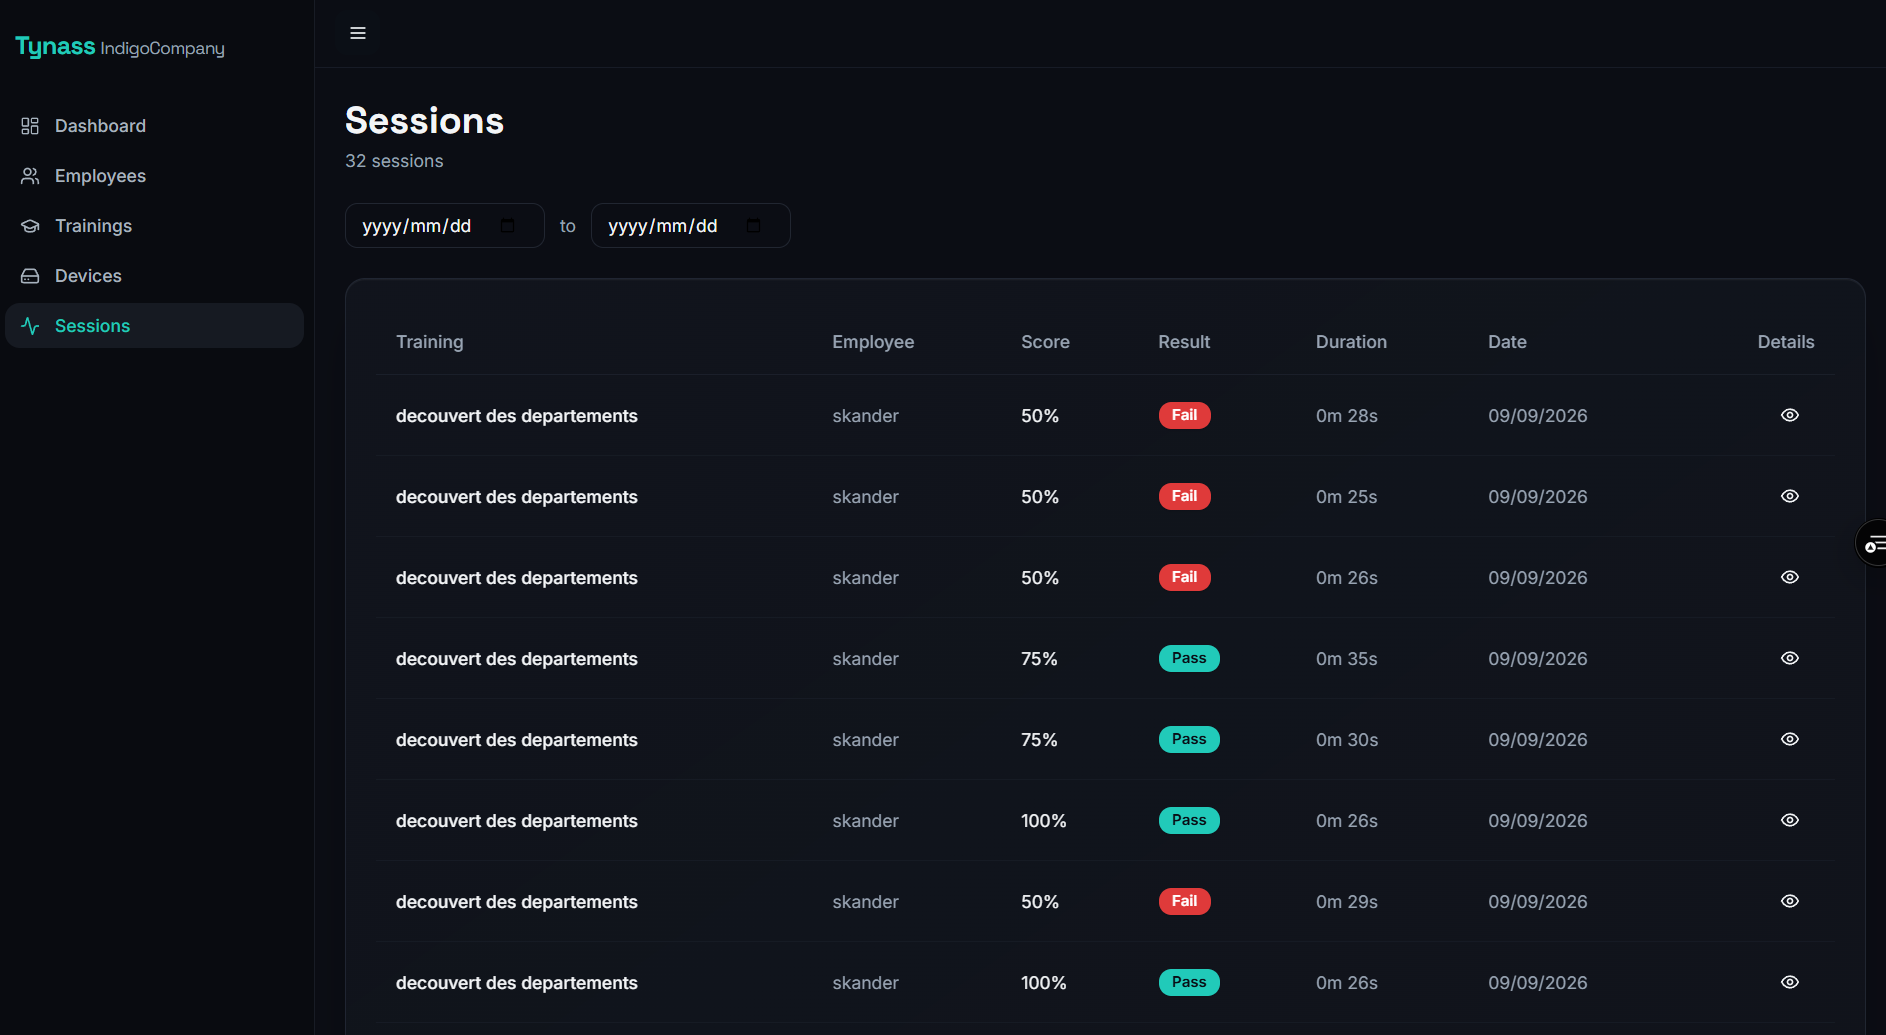
\includegraphics[width=\textwidth]{../images/dashCompany_sessions.png}
  \caption{Dashboard Company --- historique des sessions}
  \label{fig:dash_company_sessions}
\end{figure}

\section{Difficultés et solutions}

\begin{table}[H]
  \centering
  \begin{tabularx}{\textwidth}{lXX}
    \toprule
    \textbf{Défi} & \textbf{Problème} & \textbf{Solution} \\
    \midrule
    Migration router & TanStack Start (SSR) bloquait les appels
                       fetch côté client en production. &
                       Migration vers React Router v6~: routage
                       100\% côté client, sans SSR. \\
    \midrule
    Tailwind v4 & Shadcn UI incompatible avec Tailwind v4
                  (classes manquantes, styles cassés). &
                  Migration vers Tailwind v3, stable et
                  pleinement compatible avec Shadcn. \\
    \midrule
    Pattern \texttt{?? data} & Le backend enveloppe les réponses~:
                               \texttt{\{companies: [...]\}} au lieu de
                               \texttt{[...]} directement. &
                               Pattern \texttt{data.companies ?? data}
                               dans chaque appel API pour
                               rétrocompatibilité. \\
    \midrule
    Tri statistiques & Le champ \texttt{sessionsPlayed} dans les
                       mock-data ne correspondait pas au champ
                       \texttt{totalSessions} retourné par le backend. &
                       Correction du tri~: utilisation de
                       \texttt{totalSessions} (champ backend réel). \\
    \midrule
    CORS & Le dashboard (localhost:8080) était bloqué
           par le backend sans configuration CORS. &
           Ajout du middleware cors() avant toutes les
           routes, avec origines explicites. \\
    \bottomrule
  \end{tabularx}
  \caption{Difficultés rencontrées et solutions --- Itération~2}
  \label{tab:dificultes_s2}
\end{table}

\section{Évaluation de l'itération~2}

\begin{table}[H]
  \centering
  \begin{tabular}{ll}
    \toprule
    \textbf{Élément validé} & \textbf{Statut} \\
    \midrule
    Pages du dashboard Admin livrées   & 7 / 7 \\
    Pages du dashboard Company livrées & 6 / 6 \\
    Connexion des dashboards à l'API REST & Fonctionnel \\
    Déploiement en production sur Vercel & Fonctionnel \\
    \bottomrule
  \end{tabular}
  \caption{Validation fonctionnelle --- Itération~2}
  \label{tab:eval_s2}
\end{table}

Les deux dashboards sont déployés en production sur Vercel, comme le montre
la figure~\ref{fig:dashboards_vercel}.

\begin{figure}[H]
  \centering
  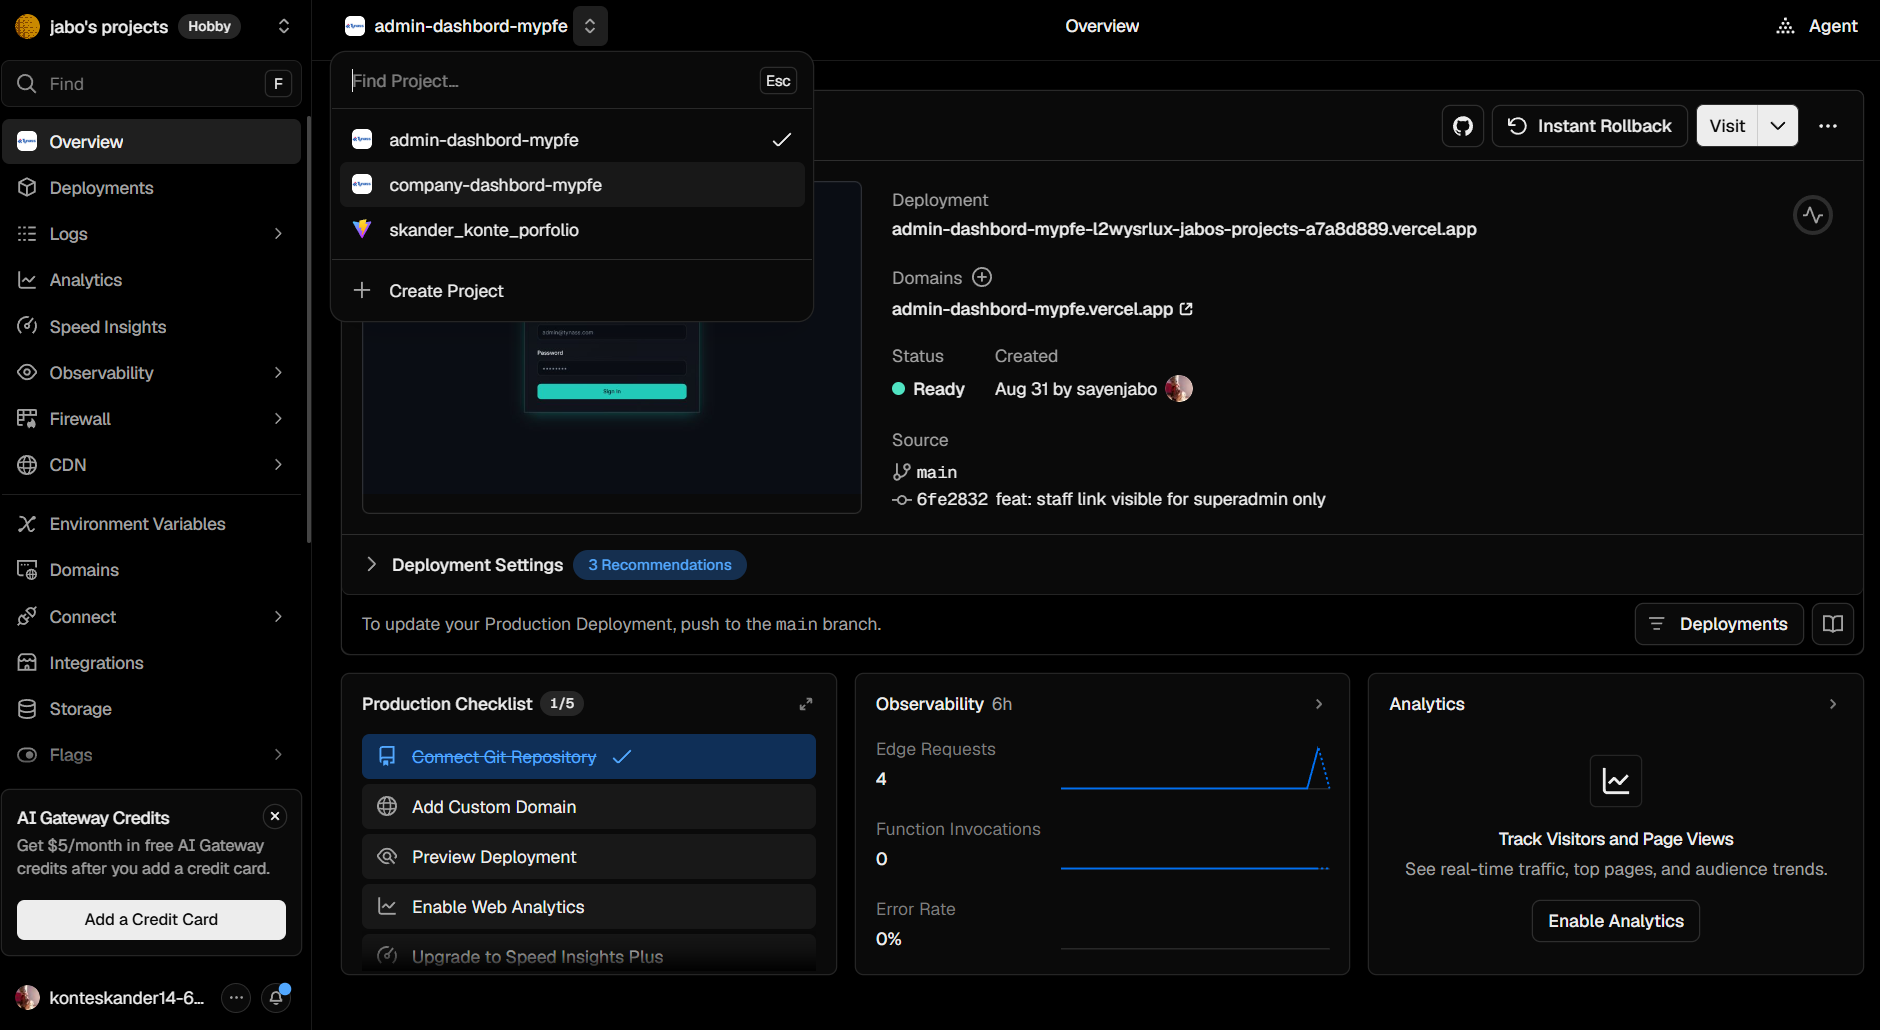
\includegraphics[width=\textwidth]{../images/dashboards_vercel.png}
  \caption{Les deux dashboards déployés en production sur Vercel}
  \label{fig:dashboards_vercel}
\end{figure}

\section{Conclusion}

Cette deuxième itération a livré les deux dashboards web de \tynassit{}, déployés sur Vercel~:
\texttt{admin-dashbord-mypfe.vercel.app} et \texttt{company-dashbord-mypfe.vercel.app}.
Les 8 user stories couvertes ont toutes été livrées. Le chapitre suivant
présente le développement de l'application VR.

% ================================================================
% chapters/chapter5.tex --- RECONSTRUCTION (même structure que ch.3)
% ----------------------------------------------------------------
% Backlog restructuré~: Titre + Charge (j/h) ajoutées, Statut retiré
% + phrase de synthèse. Charge (j/h) = MES ESTIMATIONS RELATIVES,
% pas des mesures réelles --- à remplacer si tu as de vraies données.
% Rien d'autre n'est modifié dans ce chapitre.
% ================================================================

\chapter{Itération~3 --- Application VR Meta Quest~3 (scènes d'authentification)}

\section{Introduction}

 Cette itération couvre le développement de l'application VR pour Meta Quest~3, incluant
les deux premières scènes~: la scène tutoriel (\texttt{trainingscene}, initiation aux contrôleurs) et
la scène d'authentification (\texttt{Companys}, connexion et sélection des formations). À l'issue de cette itération,
un employé peut activer le casque, se connecter, voir les formations disponibles
et accéder aux paramètres.

\section{Planification de l'itération~3}

Cette section définit les objectifs de la troisième itération, les tâches associées et
leur charge estimée.

\subsection{Objectifs}

\begin{itemize}
  \item Implémenter le flow complet d'activation du casque (Meta User ID matériel + code d'activation à 6 chiffres).
  \item Permettre le login employé (accessCode + PIN) via une interface VR intuitive.
  \item Charger et afficher les formations assignées à l'entreprise.
  \item Livrer un tutoriel d'introduction aux contrôleurs Meta Quest~3.
  \item Permettre la configuration des paramètres (audio, langue, contrôleurs).
\end{itemize}

\subsection{Tâches et estimations de l'itération~3}

\begin{table}[H]
  \centering
  \small
  \setlength{\tabcolsep}{5pt}
  \begin{tabularx}{\textwidth}{cp{3.5cm}Xc>{\footnotesize}c}
    \toprule
    \textbf{ID} & \textbf{Titre} & \textbf{Description} & \textbf{MoSCoW} & \textbf{Charge (j/h)} \\
    \midrule
    US-14 & Tutoriel des contrôleurs &
      Scène tutoriel (\texttt{trainingscene}) --- 3 leçons & \must{} & 4 \\
    US-15 & Activation du casque &
      DeviceActivationManager (Meta User ID + code d'activation) & \must{} & 2 \\
    US-16 & Connexion employé &
      EmployeeSignInPanel (code + PIN numpad) & \must{} & 3 \\
    US-17 & Liste des formations &
      ModulesPanel (grille formations) & \must{} & 2,5 \\
    US-18 & Paramètres persistants &
      SettingsPanel (audio, langue, contrôleurs) & \should{} & 3 \\
    \midrule
    \multicolumn{4}{r}{\textbf{Total estimé}} & \textbf{14,5} \\
    \bottomrule
  \end{tabularx}
  \caption{Tâches et estimations --- Itération~3}
  \label{tab:backlog_s3}
\end{table}

\noindent Toutes les user stories de cette itération ont été livrées.

\section{Conception de l'itération~3}

Cette section présente la configuration du projet Unity pour Meta Quest~3, les décisions
architecturales de l'application et l'organisation de ses scripts principaux.

\subsection{Configuration Unity~6 pour Meta Quest~3}

\begin{table}[H]
  \centering
  \begin{tabularx}{\textwidth}{lX}
    \toprule
    \textbf{Paramètre} & \textbf{Valeur} \\
    \midrule
    Plateforme cible     & Android (ARM64) \\
    API graphique        & Vulkan (recommandé Quest~3) \\
    XR Plugin            & Meta OpenXR \\
    Features activées    & Meta Quest Support, Foveated Rendering,
                           Hand Interaction Poses, XR Performance Settings \\
    Profils contrôleurs  & Meta Quest Touch Plus, Meta Quest Touch Pro \\
    Niveau API minimum   & Android 10 (API 29) \\
    \bottomrule
  \end{tabularx}
  \caption{Configuration Unity~6 pour Meta Quest~3}
  \label{tab:unity_config}
\end{table}

\subsection{Décisions architecturales --- Unity}

\begin{table}[H]
  \centering
  \begin{tabularx}{\textwidth}{lllX}
    \toprule
    \textbf{Composant} & \textbf{Retenu} & \textbf{Alternative} & \textbf{Justification} \\
    \midrule
    Moteur & Unity 6 LTS & Unreal Engine 5 & 85\% des apps Quest Store en 2024,
                                             Meta XR SDK optimisé Unity \\
    SDK    & Meta XR All-in-One & Meta Core SDK & Un seul package intégrant tous les
                                                  SDK Meta \\
    Client HTTP & TynassApiClient & ApiManager (obsolète) & Singleton avec JWT,
                                                              méthodes typées, PlayerPrefs \\
    État global & AppSession & SessionManager & Classe statique~: toujours disponible
                                                sans instanciation, pas de cycle de vie \\
    \bottomrule
  \end{tabularx}
  \caption{Décisions architecturales --- Unity}
  \label{tab:archi_unity}
\end{table}

\begin{archbox}
  \textbf{AppSession vs SessionManager}~: \texttt{SessionManager.cs} en tant que
  MonoBehaviour singleton nécessite un GameObject dans la scène et dépend du cycle
  de vie Unity. \texttt{AppSession.cs} est une classe statique C\# toujours disponible
  sans instanciation, sans \texttt{DontDestroyOnLoad}, sans risque de destruction
  entre scènes. Pour des données d'état global (token, employé connecté, formation
  active), la classe statique est architecturalement plus appropriée.
\end{archbox}

\subsection{Architecture Unity --- Scripts principaux}

L'application Unity s'organise autour de huit scripts principaux, regroupés par
responsabilité~: communication avec le backend, gestion de l'état global, navigation
entre les interfaces, et activation du casque. La figure~\ref{fig:composants_unity}
présente ces composants et leurs dépendances.

\begin{figure}[H]
  \centering
  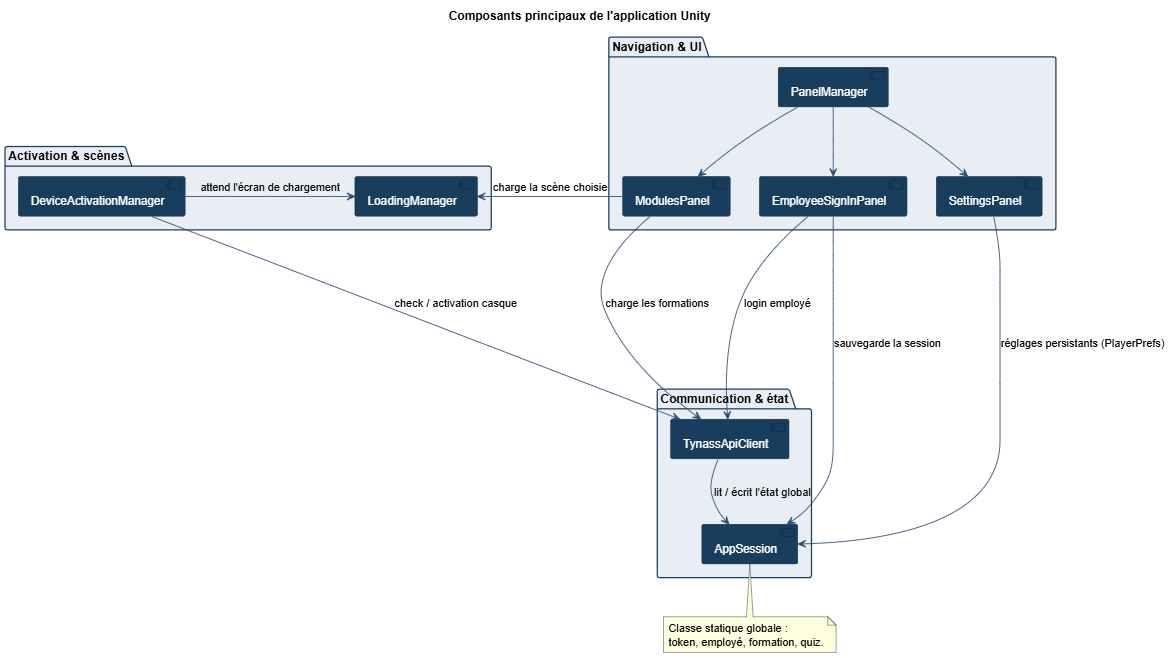
\includegraphics[width=\textwidth]{../images/composantsUnity.png}
  \caption{Diagramme de composants des scripts principaux de l'application Unity}
  \label{fig:composants_unity}
\end{figure}

Les 8 scripts principaux de l'application Unity~:

\begin{itemize}
  \item \textbf{TynassApiClient.cs}~: singleton HTTP centralisé. Gère le JWT
    (\texttt{SetToken}/\texttt{ClearToken}), \texttt{TryRestoreSession()} au
    démarrage, et toutes les méthodes typées de l'API. Utilise les classes
    \texttt{[Serializable]} pour la sérialisation JSON via \texttt{JsonUtility}.
  \item \textbf{AppSession.cs}~: classe statique globale. Stocke les données de
    Device, Company, Employee, Training et Quiz (QuizScore, QuizCorrect, QuizTotal,
    QuizCurrentIndex, QuizElapsedSecs). \texttt{AppSession.Clear()} efface les
    données personnelles de l'employé mais conserve le DeviceToken (appartient au
    casque).
  \item \textbf{PanelManager.cs}~: gère la navigation entre les panels UI
    (GoSignIn, GoEmployeePicker, GoModules, GoSettings, GoQuiz, GoQuizResult).
  \item \textbf{DeviceActivationManager.cs}~: récupère le Meta User ID via
    \texttt{Oculus.Platform.Users.GetLoggedInUser()}, orchestre le flow
    d'activation.
  \item \textbf{EmployeeSignInPanel.cs}~: gère les 2 étapes de login (Step~1~:
    accessCode XX-001, Step~2~: PIN numpad 4 chiffres).
  \item \textbf{ModulesPanel.cs}~: charge les formations via \texttt{device\_token},
    instancie les cartes de formation dans un Grid Layout Group.
  \item \textbf{SettingsPanel.cs}~: audio (master/sfx/narration/spatial), langue
    (FR/EN/AR), contrôleurs (main, dwell time, haptic). Persistance via
    \texttt{PlayerPrefs}.
  \item \textbf{TrainingSceneManager.cs}~: orchestre la scène tutoriel
    (\texttt{trainingscene})~: leçons, narration audio, NarrationManager.
\end{itemize}

\subsection{Cas d'utilisation --- Descriptions textuelles}

\begin{ucbox}{Tutoriel d'introduction (scène \texttt{trainingscene})}
  \begin{tabular}{lp{9cm}}
    \textbf{Pré-conditions} & Casque démarré, utilisateur novice en VR. \\
    \textbf{Acteur}         & Employé. \\
    \textbf{Scénario A}     &
      1. L'utilisateur choisit « Commencer les leçons » (choix A). \newline
      2. Leçon 1~: se déplacer avec le joystick jusqu'au waypoint. \newline
      3. Leçon 2~: saisir un cube (grip) et l'amener au waypoint. \newline
      4. Leçon 3~: lire un panel, cliquer sur le bouton (trigger). \newline
      5. Transition automatique vers la scène Companys. \\
    \textbf{Scénario B}     &
      1. L'utilisateur choisit « Passer » (choix B). \newline
      2. Transition directe vers la scène Companys. \\
    \textbf{Post-conditions}& Utilisateur maîtrise les 3 interactions fondamentales. \\
  \end{tabular}
\end{ucbox}

\vspace{0.5cm}

\begin{ucbox}{Sélectionner une formation (ModulesPanel)}
  \begin{tabular}{lp{9cm}}
    \textbf{Pré-conditions} & Employé connecté, \texttt{device\_token} valide. \\
    \textbf{Acteur}         & Employé. \\
    \textbf{Scénario}       &
      1. ModulesPanel appelle \texttt{GET /api/company/devices/trainings}. \newline
      2. Les formations assignées à l'entreprise sont affichées en grille. \newline
      3. L'employé pointe et sélectionne une formation. \newline
      4. \texttt{AppSession.ActiveTraining} est défini. \newline
      5. \texttt{SceneManager.LoadScene(training.sceneName)} est appelé. \newline
      6. Si \texttt{sceneName} est null~: erreur loguée, rien ne se passe. \\
    \textbf{Post-conditions}& Scène de formation chargée. \\
  \end{tabular}
\end{ucbox}

\subsection{Diagramme de séquence}

La figure~\ref{fig:flow_complet} retrace le flux complet vécu par un employé, depuis le
tutoriel jusqu'au lancement d'une simulation, en passant par l'authentification et la
sélection d'une formation. Elle montre l'enchaînement des trois scènes et leurs échanges
avec le backend.

\begin{figure}[H]
  \centering
  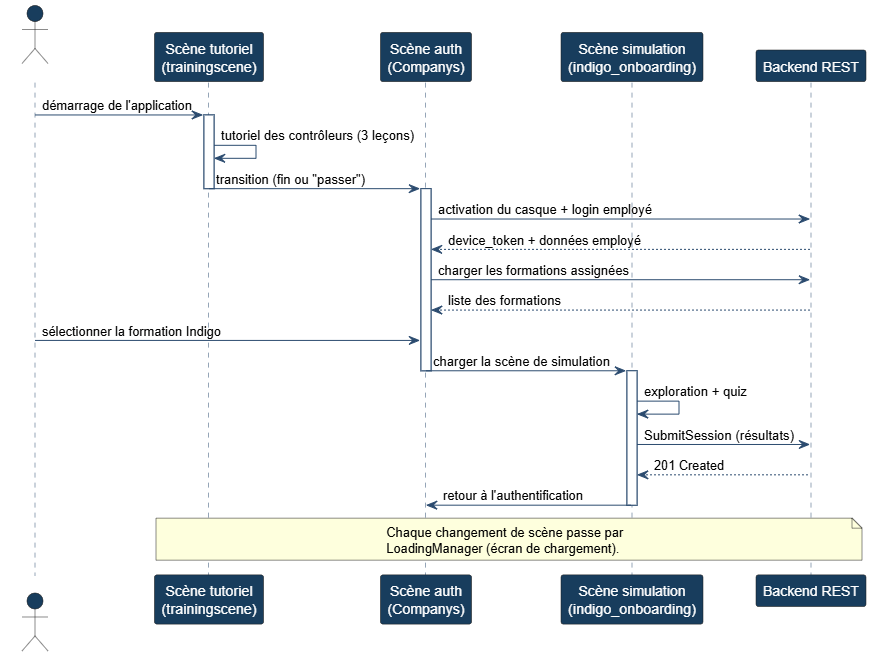
\includegraphics[width=0.9\textwidth]{../images/flowComplet.png}
  \caption{Diagramme de séquence --- flux complet entre les trois scènes}
  \label{fig:flow_complet}
\end{figure}

\section{Implémentation de l'itération~3}

Cette section détaille la mise en œuvre des principaux composants de l'application~: le
client HTTP, l'activation du casque, le login employé et les panneaux de l'interface.

\subsection{TynassApiClient.cs --- Client HTTP centralisé}

\texttt{TynassApiClient} est le singleton central de communication avec le backend.
Sa conception résout un problème fondamental de Unity~: \texttt{JsonUtility} ne
sérialise que les classes marquées \texttt{[Serializable]}. Tout objet anonyme
produit un JSON vide (\texttt{\{\}}).

 \begin{lstlisting}[language={[Sharp]C}, caption={TynassApiClient -- methode typee async}]
[Serializable]
public class EmployeeLoginPayload {
    public string accessCode;
    public string pin;
}

public async Task<EmployeeLoginResponse> LoginEmployee(
    string accessCode, string pin, string deviceToken)
{
    var payload = new EmployeeLoginPayload { accessCode = accessCode, pin = pin };
    // POST /company/employees/login avec le device_token dans l'en-tete
    return await PostRequest<EmployeeLoginResponse>(
        "/company/employees/login", payload, deviceToken);
}
\end{lstlisting}

\subsection{DeviceActivationManager --- Meta User ID}

\begin{lstlisting}[language={[Sharp]C}, caption={Meta User ID -- recuperation et verification}]
Oculus.Platform.Users.GetLoggedInUser().OnComplete(async msg => {
    string metaUserId;
    if (!msg.IsError)
        metaUserId = msg.Data.ID.ToString();
    else
        metaUserId = SystemInfo.deviceUniqueIdentifier; // fallback editeur

    var response = await TynassApiClient.Instance.CheckDevice(metaUserId);
    if (response != null && response.status == "activated")
        ShowLoginPanel();
    else
        ShowActivationPanel();
});
\end{lstlisting}

\subsection{EmployeeSignInPanel --- Login en 2 étapes}

\begin{enumerate}
  \item \textbf{Step 1 --- accessCode}~: l'employé saisit son code via un clavier
    alphanumérique. Unity valide le format en temps réel avec
    \texttt{Regex.IsMatch(code, \^{}[A-Z]\{2\}-\textbackslash d\{3\}\$)}.
    Cette validation côté Unity donne un retour immédiat sans aller-retour réseau.
    La validation backend constitue la sécurité réelle (défense en profondeur).
  \item \textbf{Step 2 --- PIN}~: numpad 4 chiffres (0-9 + effacer). Visuellement
    masqué par des étoiles. Envoyé au backend pour vérification bcrypt.
\end{enumerate}

\begin{figure}[H]
  \centering
  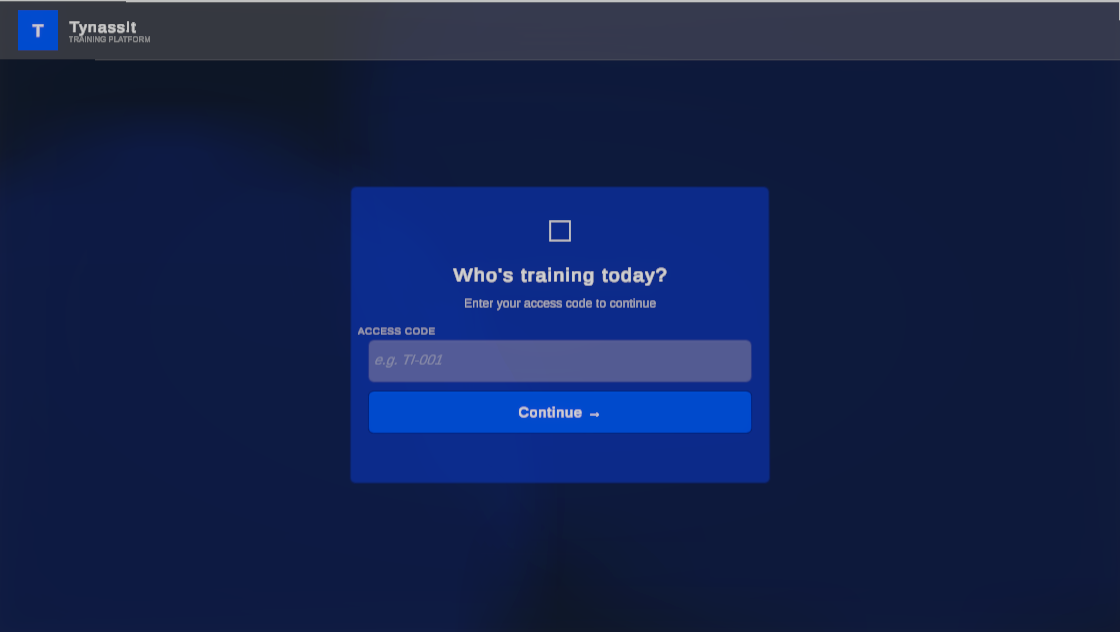
\includegraphics[width=0.7\textwidth]{../images/vr_signin_code.png}
  \caption{Connexion employé --- saisie du code d'accès}
  \label{fig:vr_signin_code}
\end{figure}

\begin{figure}[H]
  \centering
  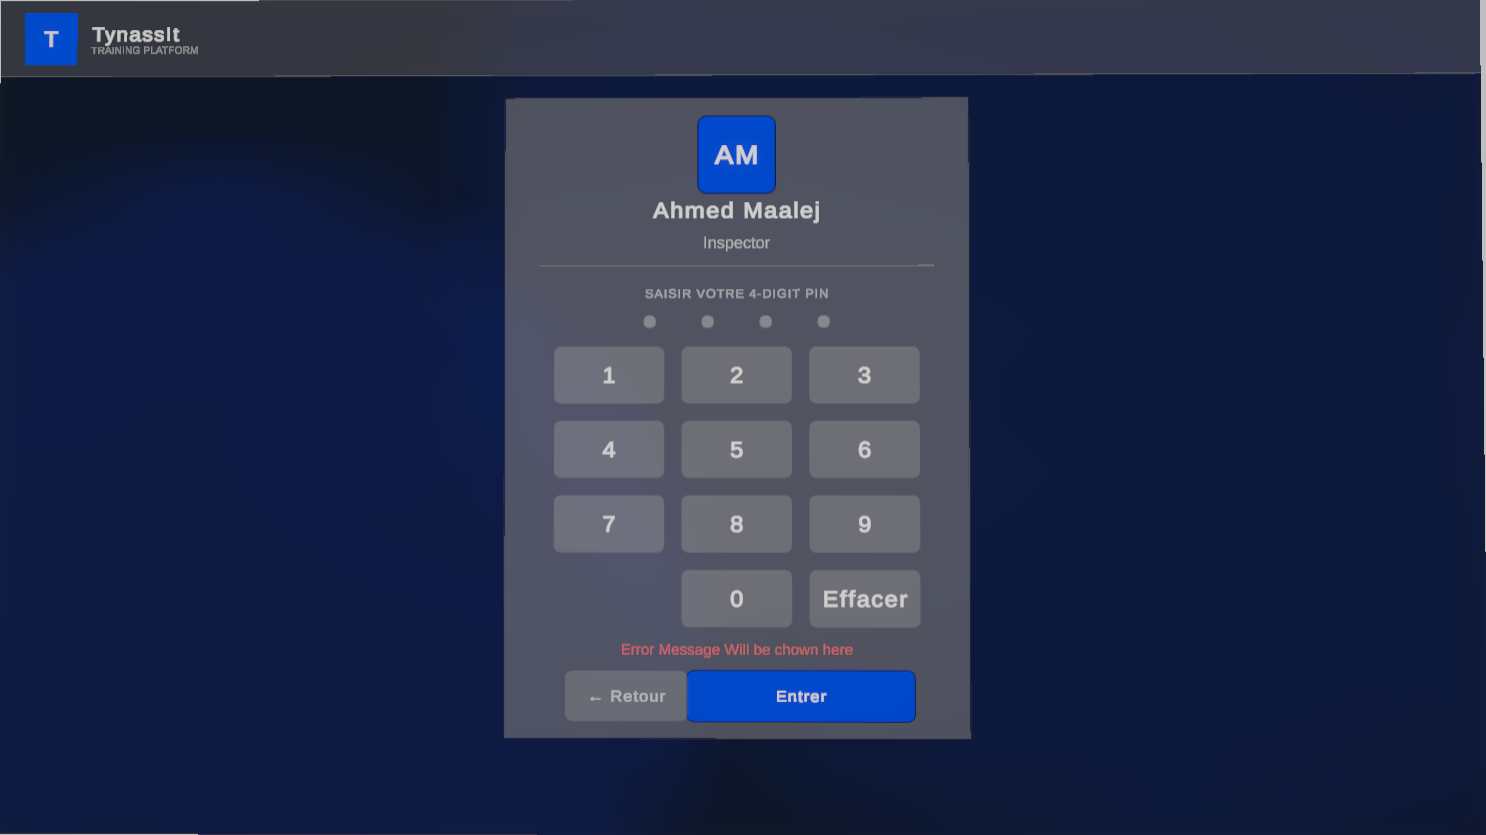
\includegraphics[width=0.7\textwidth]{../images/vr_signin_pin.png}
  \caption{Connexion employé --- saisie du PIN}
  \label{fig:vr_signin_pin}
\end{figure}

\subsection{ModulesPanel --- Grille des formations}

Les cartes de formation sont instanciées dynamiquement depuis un prefab dans un
\textbf{Grid Layout Group}, qui calcule automatiquement la position de chaque enfant
selon \texttt{Cell Size} et \texttt{Spacing}.

\begin{figure}[H]
  \centering
  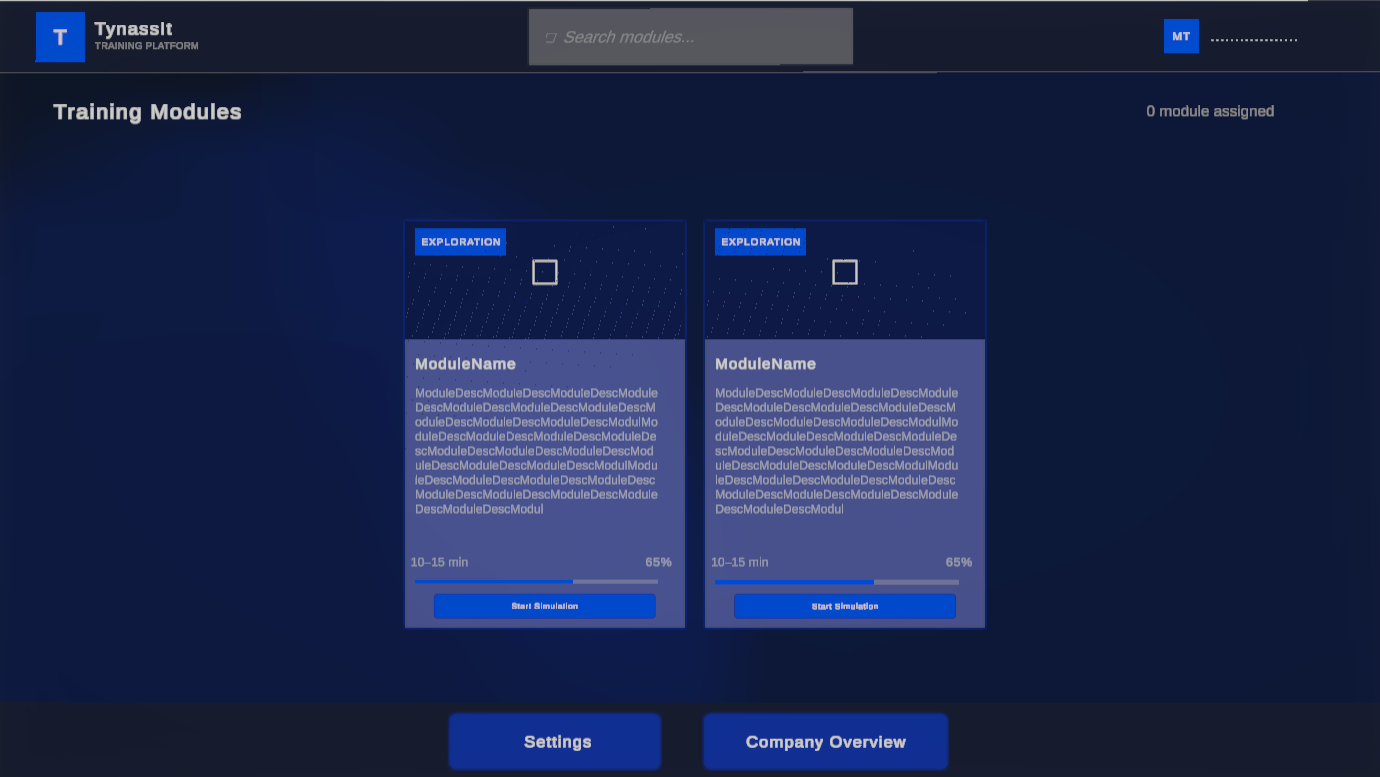
\includegraphics[width=0.8\textwidth]{../images/vr_modules.png}
  \caption{Liste des formations assignées (ModulesPanel)}
  \label{fig:vr_modules}
\end{figure}

\subsection{SettingsPanel --- Paramètres persistants}

Tous les paramètres sont sauvegardés dans \texttt{PlayerPrefs}~:
\texttt{vol\_master}, \texttt{vol\_sfx}, \texttt{vol\_narr}, \texttt{mute\_all},
\texttt{spatial}, \texttt{ui\_lang}, \texttt{narr\_lang}, \texttt{hand},
\texttt{dwell\_time}, \texttt{glow}, \texttt{haptic}.

\begin{figure}[H]
  \centering
  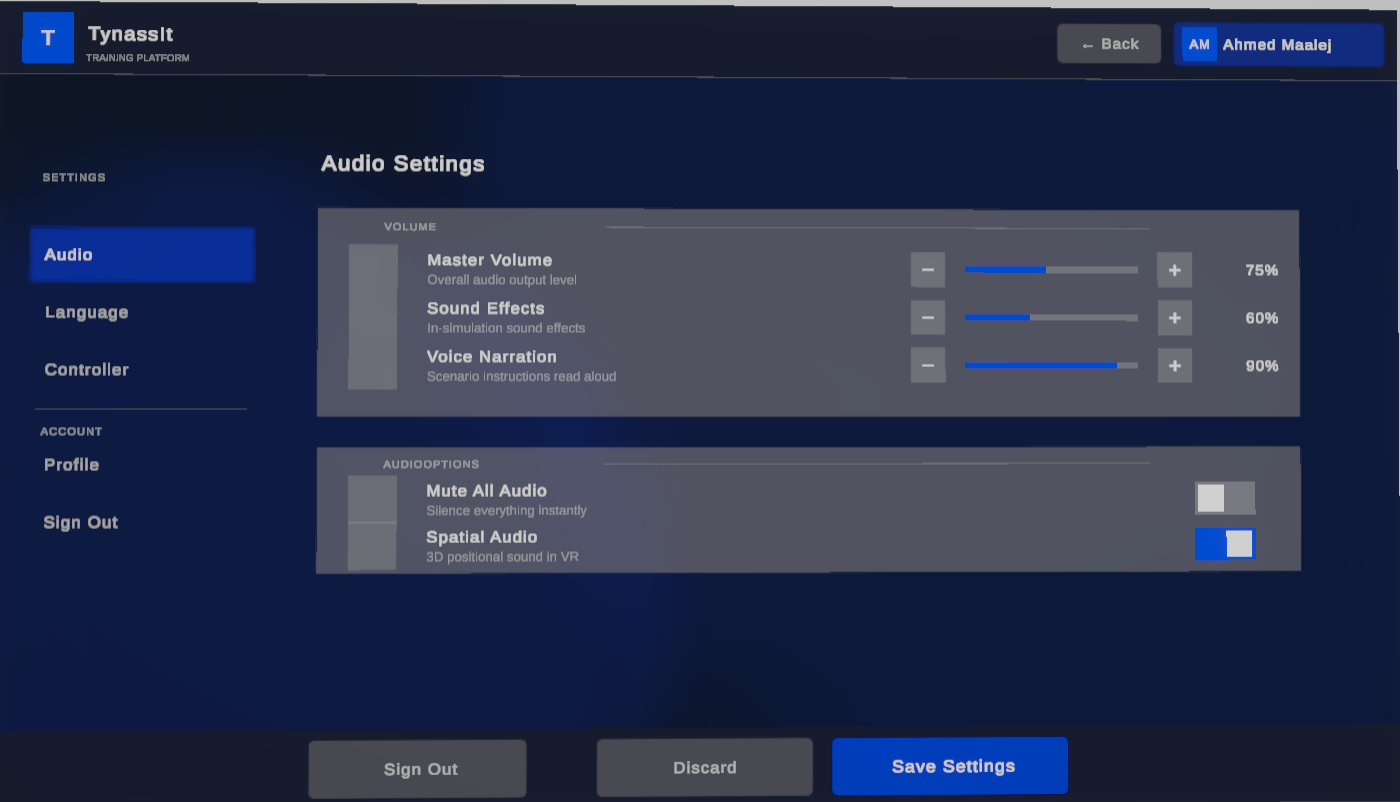
\includegraphics[width=0.8\textwidth]{../images/vr_settings.png}
  \caption{Panneau de configuration des paramètres}
  \label{fig:vr_settings}
\end{figure}

\section{Difficultés et solutions}

\begin{table}[H]
  \centering
  \begin{tabularx}{\textwidth}{lXX}
    \toprule
    \textbf{Défi} & \textbf{Problème} & \textbf{Solution} \\
    \midrule
    JsonUtility & Les objets anonymes \texttt{new \{email = "test"\}}
                  produisaient \texttt{\{\}} (JSON vide). &
                  Création de classes \texttt{[Serializable]} explicites
                  pour tous les payloads. \\
    \midrule
    Vidéos lentes & Les vidéos dans \texttt{Resources/} étaient préchargées
                    au démarrage, causant un gel de plus d'une minute. &
                    Migration vers \texttt{StreamingAssets/}~: lecture en
                    streaming via URL \texttt{file://}, démarrage instantané. \\
    \midrule
    Cards superposées & Les cartes de formations apparaissaient toutes
                        au même point (0,0,0) sans layout automatique. &
                        \texttt{Grid Layout Group} calcule automatiquement
                        la position de chaque carte. \\
    \midrule
    Vélocité locomotion & Maintenir le joystick pendant un blocage
                          accumulait une vélocité~: l'employé partait
                          en sprint au déblocage. &
                          \texttt{EnableMovement()} remet la vélocité
                          à zéro avant de réactiver le mouvement. \\
    \bottomrule
  \end{tabularx}
  \caption{Difficultés rencontrées et solutions --- Itération~3}
  \label{tab:dificultes_s3}
\end{table}

\section{Évaluation de l'itération~3}

\begin{table}[H]
  \centering
  \begin{tabularx}{\textwidth}{Xl}
    \toprule
    \textbf{Élément validé} & \textbf{Statut} \\
    \midrule
    Activation du casque sur Meta Quest~3 & Fonctionnel \\
    Login employé (code d'accès + PIN) sur le casque & Fonctionnel \\
    Affichage des formations assignées & Fonctionnel \\
    Tutoriel des contrôleurs (3 leçons) & 3 / 3 \\
    Persistance des paramètres (audio, langue, contrôleurs) & Fonctionnel \\
    \bottomrule
  \end{tabularx}
  \caption{Validation fonctionnelle --- Itération~3}
  \label{tab:eval_s3}
\end{table}

La figure~\ref{fig:vr_tuto} illustre la deuxième leçon du tutoriel, où
l'employé apprend à saisir un objet.

\begin{figure}[H]
  \centering
  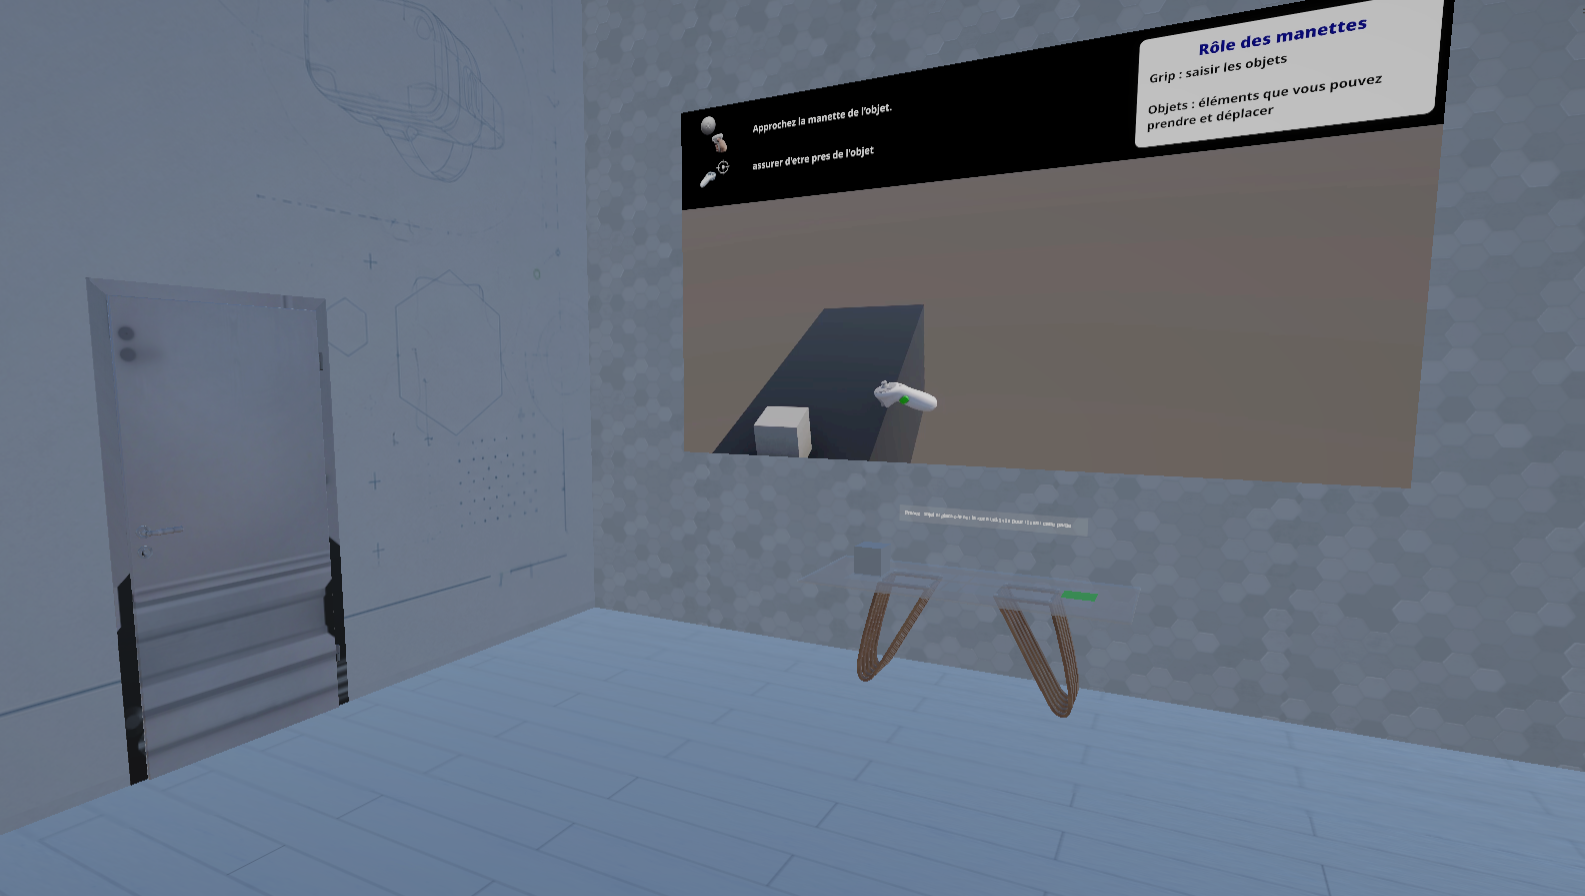
\includegraphics[width=0.8\textwidth]{../images/vr_tutoriel_grip.png}
  \caption{Scène tutoriel --- leçon de manipulation (grip)}
  \label{fig:vr_tuto}
\end{figure}

\begin{figure}[H]
  \centering
  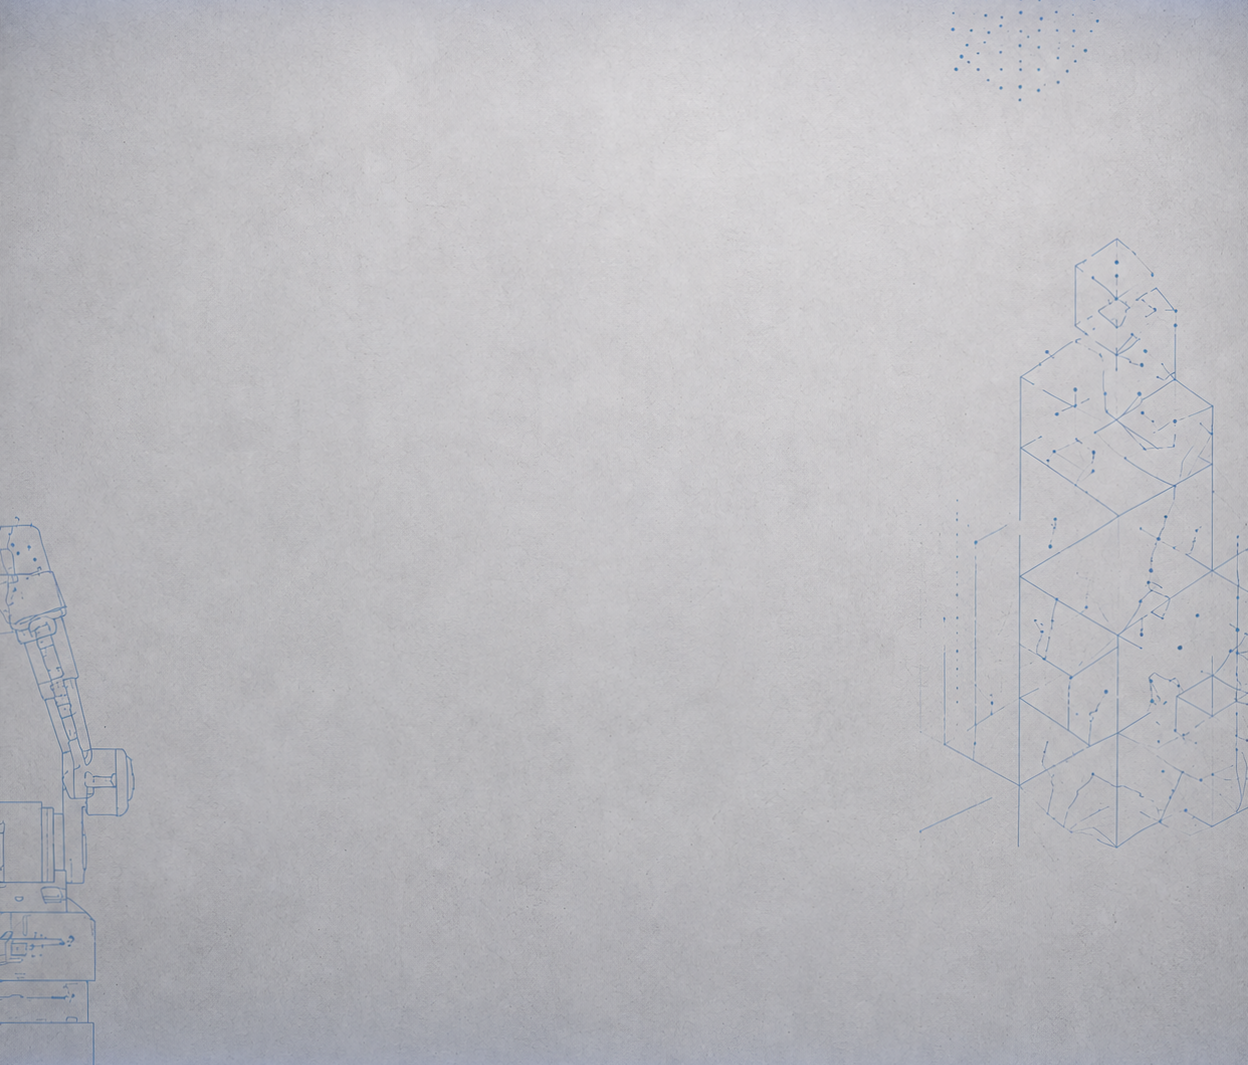
\includegraphics[width=0.9\textwidth]{../images/vr_flow_casque.png}
  \caption{Exécution du flux complet sur le casque Meta Quest~3}
  \label{fig:vr_flow_casque}
\end{figure}

\section{Conclusion}

Cette troisième itération a livré l'application VR avec ses deux premières scènes~:
le tutoriel des contrôleurs et l'authentification. Le flow complet
fonctionne sur le casque physique Meta Quest~3~: activation, login employé, affichage
des formations. Le chapitre suivant présente la simulation d'intégration d'Indigo Company.

% ================================================================
% chapters/chapter6.tex --- RECONSTRUCTION
% ----------------------------------------------------------------
% Assemblé à partir des fragments retrouvés dans le project knowledge
% au fil de cette conversation, PAS une copie directe et vérifiée
% d'un seul fichier source. Fais un diff rapide contre ton fichier
% réel avant d'écraser l'original, par sécurité.
%
% CE QUI EST FUSIONNÉ ICI (déjà appliqué) :
%   - Objectifs : 2 phases au lieu de 3 (bloc itemize complet, pas
%     de "Lonely \item")
%   - Structure de la simulation : 2 phases (Exploration, Quiz)
%   - Mapping : SessionPayload -> SessionSubmitPayload, partout
%     y compris dans le use case "Soumettre une session"
%   - Cas d'utilisation "Vivre la simulation intigo" : renuméroté
%     sur 2 phases
%   - Code listing SimulationManager.cs : remplacé par le vrai
%     QuizManager.EndQuizAsync() (async/await, SessionSubmitPayload,
%     device token explicite) --- l'ancien listing montrait encore
%     un style coroutine + callbacks qui ne correspond ni à l'ancien
%     ni au nouveau code réel
%   - Conclusion du chapitre : nuancée ("en cours de finalisation"
%     au lieu de "fonctionne de bout en bout")
%
% CE QUI N'EST PAS TOUCHÉ (attend ta confirmation / tes vraies
% mesures) :
%   - Backlog du sprint 4 (tableau 6.2.2) : checkmarks inchangés
%   - Difficultés et solutions : inchangé
%   - Évaluation du sprint 4 : toujours "---", à remplir avec les
%     vraies mesures une fois testé sur casque
% ================================================================

\chapter{Itération~4 --- Simulation VR d'intégration Indigo Company}

\section{Introduction}

Cette quatrième itération représente le cœur fonctionnel de \tynassit{}~: la simulation VR
d'intégration des nouveaux employés d'\textbf{Indigo Company}. Cette scène plonge le nouvel employé dans un environnement 3D fidèle aux locaux d'Indigo, lui fait découvrir les différents départements accompagnés de narrations audio, puis évalue sa compréhension par un quiz. À la fin de la simulation,
les résultats sont automatiquement soumis à la plateforme \tynassit{}.

\section{Planification de l'itération~4}

Cette section définit les objectifs de la dernière itération, les tâches associées et
leur charge estimée.

\subsection{Objectifs}

\begin{itemize}
  \item Modéliser et optimiser l'environnement 3D Indigo Company dans Blender.
  \item Importer et intégrer l'environnement dans Unity~6.
  \item Développer les 2 phases de la simulation (exploration des locaux, quiz).
  \item Implémenter le système de quiz avec calcul automatique du score.
  \item Connecter la fin de simulation à \texttt{TynassApiClient.SubmitSession()}.
  \item Afficher les résultats dans le panel QuizResult.
\end{itemize}

\subsection{Tâches et estimations de l'itération~4}

\begin{table}[H]
  \centering
  \begin{tabularx}{\textwidth}{lp{2.8cm}Xcc}
    \toprule
    \textbf{ID} & \textbf{Titre} & \textbf{Description} & \textbf{MoSCoW} & \textbf{Charge estimée (j/h)} \\
    \midrule
    US-19 & Exploration des locaux &
      Environnement 3D Indigo (Blender + optimisation Quest~3) & \must{} & 8 \\
    US-20 & Quiz de fin de simulation &
      Simulation~: exploration + quiz & \must{} & 5 \\
    US-21 & Soumission automatique des résultats &
      SubmitSession → backend → visible dashboard & \must{} & 2 \\
    US-22 & Affichage des résultats &
      Panel QuizResult (score + critères) & \must{} & 1,5 \\
     US-23 & Navigation dans la liste des formations &
      Scroll VR joystick dans ModulesPanel & \could{} & 1 \\
    US-24 & Gestion des quiz &
      Interface entreprise~: création de quiz par formation & \must{} & 3 \\
    US-25 & Objectifs de formation &
      Milestones par employé (statut auto après session) & \should{} & 2 \\
    \midrule
    \multicolumn{4}{r}{\textbf{Total estimé}} & \textbf{22,5} \\
    \bottomrule
  \end{tabularx}
  \caption{Tâches et estimations --- Itération~4}
  \label{tab:backlog_s4}
\end{table}

\noindent US-19 à US-22, US-24 et US-25 ont été livrées~; US-23 reste en cours.

\section{Conception de l'itération~4}

Cette section présente la conception de la simulation~: la modélisation 3D de
l'environnement Indigo, la structure des deux phases, le système de quiz et la
correspondance des données transmises au backend.

\subsection{Modélisation 3D --- Blender}

L'environnement 3D d'Indigo Company a été modélisé dans \textbf{Blender} sur la base
des plans réels des locaux fournis par Indigo Company, puis exporté en FBX et importé
dans Unity~6.

Les optimisations appliquées pour Meta Quest~3~:

\begin{itemize}
  \item \textbf{Polygon count}~: inférieur à 500\,000 triangles pour la scène complète.
  \item \textbf{Textures}~: format ASTC 6x6 pour les grandes surfaces, ASTC 4x4 pour
    les textures détaillées.
  \item \textbf{Éclairage}~: \textit{baked lighting} (pas d'éclairage dynamique en
    temps réel), lightmaps calculées dans Unity.
  \item \textbf{Static Batching}~: activé sur tous les objets statiques pour réduire
    les draw calls.
  \item \textbf{Occlusion Culling}~: activé pour ne rendre que les objets visibles
    depuis la position courante.
\end{itemize}

\placeholder{Environnement Blender --- vue isométrique (à insérer)}

\placeholder{Environnement importé dans Unity~6 (à insérer)}

\subsection{Structure de la simulation}

 La simulation d'intégration Indigo (\texttt{indigo\_onboarding}) est organisée en \textbf{2 phases séquentielles}~:

\begin{enumerate}
  \item \textbf{Phase 1 --- Exploration des locaux}~: l'employé navigue librement dans les locaux d'Indigo Company et découvre huit zones interactives~--- les sept départements ainsi qu'une zone dédiée au responsable de département ---, chacune
présentée par un panneau d'information et une narration audio.
 \item \textbf{Phase 2 --- Quiz}~: questions à choix multiples évaluant la
    compréhension des informations présentées lors de l'exploration. Le nombre
    et le contenu des questions sont définis par l'entreprise depuis son tableau de bord.
\end{enumerate}

\begin{figure}[H]
  \centering
  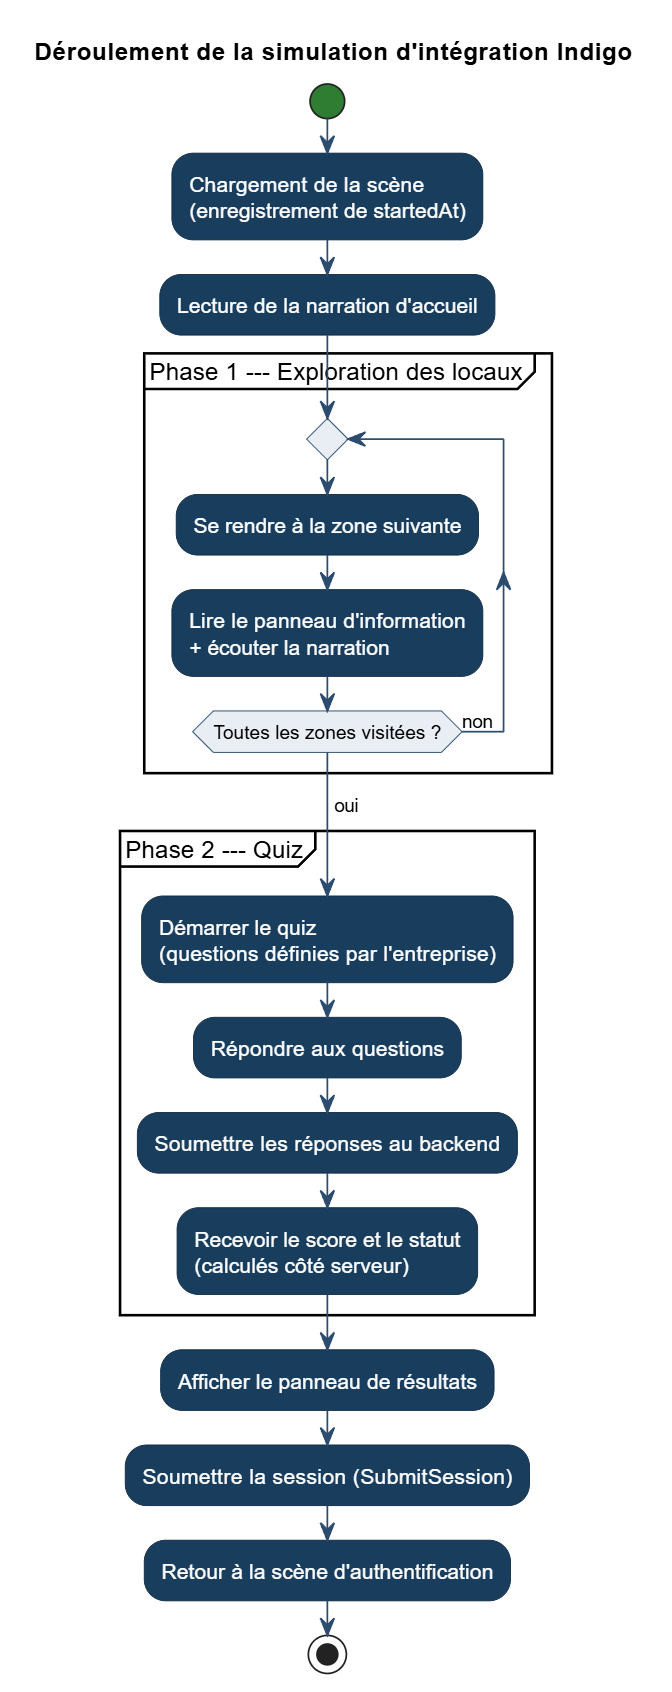
\includegraphics[width=0.7\textwidth]{../images/activiteSimulation.png}
  \caption{Diagramme d'activité --- déroulement de la simulation en deux phases}
  \label{fig:activite_simulation}
\end{figure}

\subsection{Système de quiz}

Les questions du quiz et leur nombre sont définis par l'entreprise cliente depuis son tableau de bord~; ils ne sont pas figés dans l'application. Le casque transmet les réponses de l'employé au backend via \texttt{POST /company/quiz/submit}~; le backend
les valide 
--- les bonnes réponses ne sont jamais envoyées au casque, ce qui empêche toute triche 
--- puis renvoie le score et le statut de réussite. Le score est calculé selon~:

\[
  \text{Score} = \frac{\text{QuizCorrect}}{\text{QuizTotal}} \times 100
\]

\[
  \text{passed} = \text{Score} \geq \text{passingScore}
\]
où \texttt{passingScore} est le seuil de réussite défini par l'entreprise, fixé à 70~\% par défaut.
\subsection{Mapping AppSession → SessionSubmitPayload}

\begin{table}[H]
  \centering
  \begin{tabularx}{\textwidth}{lX}
    \toprule
    \textbf{Champ SessionSubmitPayload} & \textbf{Source dans AppSession / Unity} \\
    \midrule
    \texttt{trainingId}       & \texttt{AppSession.ActiveTraining.\_id} \\
    \texttt{employeeId}       & \texttt{AppSession.EmployeeId} \\
    \texttt{startedAt}        & \texttt{DateTime.UtcNow} au chargement de la scène \\
    \texttt{completedAt}      & \texttt{DateTime.UtcNow} à la fin du quiz \\
    \texttt{score}            & \texttt{AppSession.QuizScore} (retourné par le backend) \\
    \texttt{passed}           & \texttt{AppSession.QuizPassed} (retourné par le backend) \\
    \texttt{evaluationCriteria[]} & Actions évaluées pendant la simulation \\
    \bottomrule
  \end{tabularx}
  \caption{Correspondance AppSession --- SessionSubmitPayload}
  \label{tab:session_mapping}
\end{table}

\subsection{Cas d'utilisation --- Descriptions textuelles}

\clearpage

\begin{ucbox}{Vivre la simulation d'intégration Indigo}
  \begin{tabular}{lp{9cm}}
    \textbf{Pré-conditions} & Employé connecté, formation d'intégration Indigo sélectionnée. \\
    \textbf{Acteur}         & Employé (via Meta Quest~3). \\
    \textbf{Scénario}       &
      1. La scène d'intégration Indigo est chargée via \texttt{LoadingScreen}. \newline
      2. \texttt{OnboardingManager} enregistre \texttt{startedAt = DateTime.UtcNow}. \newline
       3. Phase 1~: Employé explore les locaux et les huit zones
         (sept départements + responsable~; navigation + panneaux + narrations). \newline
      4. Phase 2~: Quiz séquentiel (questions définies par l'entreprise). \newline
      5. À la fin~: QuizManager appelle \texttt{SubmitSession()}. \newline
      6. PanelManager.GoQuizResult() affiche les résultats. \\
    \textbf{Post-conditions}& Session stockée en BDD, visible dans dashboard admin. \\
  \end{tabular}
\end{ucbox}

\vspace{0.5cm}

\begin{ucbox}{Soumettre une session (SubmitSession)}
  \begin{tabular}{lp{9cm}}
    \textbf{Pré-conditions} & Simulation terminée, AppSession remplie. \\
    \textbf{Acteur}         & QuizManager (automatique). \\
    \textbf{Scénario}       &
      1. Construire \texttt{SessionSubmitPayload} depuis AppSession. \newline
      2. Appel \texttt{TynassApiClient.SubmitSession(...)}. \newline
      3. Backend calcule \texttt{durationSeconds} (côté serveur). \newline
      4. Backend incrémente \texttt{attemptNumber} (pre-save hook). \newline
      5. Session stockée en MongoDB. \newline
      6. Réponse 201 Created → GoQuizResult(). \\
    \textbf{Exceptions}     & Perte Wi-Fi → retry automatique (3 tentatives). \\
    \textbf{Post-conditions}& Session visible dans les dashboards Admin et Company. \\
  \end{tabular}
\end{ucbox}

\begin{figure}[H]
  \centering
  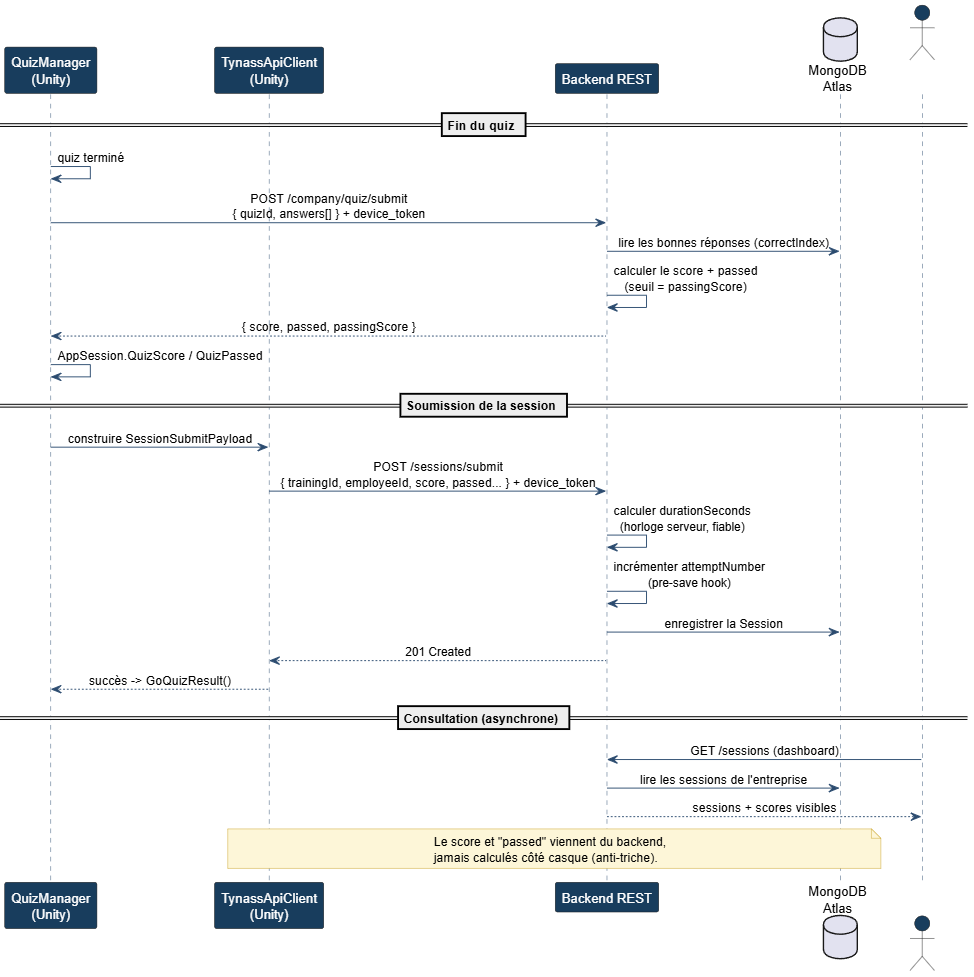
\includegraphics[width=0.9\textwidth]{../images/seqSubmit.png}
  \caption{Diagramme de séquence --- soumission d'une session}
  \label{fig:seq_submit}
\end{figure}

\section{Implémentation de l'itération~4}

Cette section détaille la mise en œuvre de la simulation~: les gestionnaires
d'orchestration et de quiz, puis le panneau d'affichage des résultats.

\subsection{OnboardingManager.cs et QuizManager.cs}

\texttt{OnboardingManager} orchestre l'exploration des huit zones (Phase~1). À la
fin de cette séquence, il délègue au \texttt{QuizManager} le déclenchement du quiz
(Phase~2) et la soumission finale des résultats~:

\begin{lstlisting}[language={[Sharp]C}, caption={QuizManager --- fin du quiz et SubmitSession}]
private async Task EndQuizAsync() {
    quizActive = false;
    quizPanel.SetActive(false);

    // Pourcentage, jamais le nombre brut de bonnes reponses
    AppSession.QuizScore = Mathf.RoundToInt(
        AppSession.QuizCorrect * 100f / AppSession.QuizTotal);
    bool passed = AppSession.QuizScore >= AppSession.PassingScore;

    string deviceToken = AppSession.DeviceToken;
    if (string.IsNullOrEmpty(deviceToken))
        deviceToken = PlayerPrefs.GetString("device_token", "");

    var result = await TynassApiClient.Instance.SubmitSession(
        trainingId:  AppSession.ActiveTraining?._id,
        employeeId:  AppSession.IsGuest ? null : AppSession.EmployeeId,
        startedAt:   AppSession.SimulationStartedAt,
        completedAt: DateTime.UtcNow,
        score:       AppSession.QuizScore,
        passed:      passed,
        deviceToken: deviceToken
    );

    if (result == null)
        Debug.LogError("SubmitSession a echoue");

    PanelManager.Instance.GoQuizResult();
}
\end{lstlisting}

\subsection{Panel QuizResult}

Le panel QuizResult affiche~:
\begin{itemize}
  \item Le score final en pourcentage.
  \item Le \textbf{statut}~: \og Réussi \fg{} (vert) ou \og Échoué \fg{} (rouge).
  \item Le détail des \textbf{critères d'évaluation} (procédure, identification,
    décision, temps).
  \item Un bouton \og Retour aux formations \fg{} et un bouton \og Se déconnecter \fg{}.
\end{itemize}

\placeholder{Capture Panel QuizResult --- score et critères (à insérer)}

\section{Difficultés et solutions}

\begin{table}[H]
  \centering
  \begin{tabularx}{\textwidth}{lXX}
    \toprule
    \textbf{Défi} & \textbf{Problème} & \textbf{Solution} \\
    \midrule
    Optimisation polygones & L'environnement complet dépassait
                             500\,000 polygones, causant des chutes
                             de FPS sur Meta Quest~3. &
                             Décimation des meshes dans Blender,
                             activation du LOD Group pour les
                             objets distants. \\
    \midrule
    Artefacts lightmap & Les baked lightmaps calculées dans Blender
                         n'étaient pas transférées correctement en
                         FBX vers Unity. &
                         Recalcul des lightmaps directement dans Unity
                         avec la Progressive Lightmapper. \\
    \midrule
    Timer quiz & La synchronisation entre QuizElapsedSecs et
                 les transitions de questions causait des décalages. &
                 Timer géré dans AppSession avec
                 \texttt{Time.deltaTime} indépendant des transitions. \\
    \bottomrule
  \end{tabularx}
  \caption{Difficultés rencontrées et solutions --- Itération~4}
  \label{tab:dificultes_s4}
\end{table}

\section{Évaluation de l'itération~4}

\begin{table}[H]
  \centering
  \begin{tabularx}{\textwidth}{Xl}
    \toprule
    \textbf{Élément validé} & \textbf{Statut} \\
    \midrule
    Exploration des 8 zones (7 départements + responsable) & Fonctionnel \\
    Narrations audio intégrées à la scène & Fonctionnel \\
    Quiz à choix multiples, score calculé côté backend & Fonctionnel \\
    Soumission automatique de session (\texttt{SubmitSession}) & Validé \\
    Session visible dans le dashboard d'administration & Validé \\
    Taille de l'APK & 2,4~Go \\
    \bottomrule
  \end{tabularx}
  \caption{Validation fonctionnelle --- Itération~4}
  \label{tab:eval_s4}
\end{table}

\placeholder{Capture environnement 3D Indigo dans Unity (à insérer)}

\placeholder{Capture quiz en VR --- question à choix multiples (à insérer)}

\placeholder{Capture session visible dans le dashboard admin (à insérer)}

\section{Conclusion}

Cette quatrième itération constitue le cœur du module de formation Indigo~:
modélisation complète de l'environnement 3D, narrations intégrées à la scène, système
de quiz fonctionnel et soumission automatique des résultats via \texttt{SubmitSession}.
Restent à finaliser la validation des tests sur casque et la mesure des métriques de
performance. Une fois ces vérifications effectuées, la simulation d'intégration d'Indigo
Company couvrira l'intégralité du parcours~: de l'exploration immersive des locaux
jusqu'à la remontée automatique des résultats dans le dashboard d'administration. Le
chapitre suivant présente la conclusion générale et les perspectives du projet.

\chapter*{Conclusion générale et perspectives}
\addcontentsline{toc}{chapter}{Conclusion générale et perspectives}
\markboth{Conclusion générale et perspectives}{}

\section*{Récapitulatif des réalisations}

Ce projet de fin d'études a abouti au développement complet de \tynassit{},
une plateforme B2B de formation en Réalité Virtuelle sur Meta Quest~3.
Les quatre sprints ont livré les réalisations suivantes~:

\begin{itemize}
  \item \textbf{Sprint~1 --- Backend}~: API REST complète (30+ endpoints), 7 modèles
    MongoDB, architecture de sécurité à 4 couches (JWT différencié, RBAC, bcrypt,
    SHA-256), système d'activation de casques via Meta User ID, login employé
    (accessCode XX-001 + PIN). Déployé sur Render.

  \item \textbf{Sprint~2 --- Dashboards}~: dashboard Admin (7 pages, React + TypeScript)
    et dashboard Company (6 pages). Gestion complète des entreprises, formations,
    casques, employés et statistiques. Déployés sur Vercel.

  \item \textbf{Sprint~3 --- Unity Auth}~: scène trailler (tutoriel 3 leçons) et
    scène Companys (activation casque, login employé, sélection formations, paramètres).
    Architecture Unity avec TynassApiClient, AppSession, PanelManager.

  \item \textbf{Sprint~4 --- Simulation Indigo}~: simulation VR d'intégration des
    nouveaux employés (3 phases~: exploration, mise en situation, quiz), soumission
    automatique des résultats à \tynassit{}, panel QuizResult.
\end{itemize}

\section*{Bilan personnel}

Ce projet a permis d'acquérir et d'approfondir des compétences dans des domaines variés~:

\begin{itemize}
  \item \textbf{Développement VR}~: Unity~6, Meta XR SDK, OpenXR, optimisation Quest~3,
    modélisation Blender, animation 3D.
  \item \textbf{Backend}~: Node.js, Express, MongoDB, Mongoose, JWT, bcrypt, SHA-256,
    architecture REST, déploiement cloud.
  \item \textbf{Frontend}~: React, TypeScript, TanStack Query, Shadcn UI, Tailwind.
  \item \textbf{Gestion de projet}~: méthodologie Scrum, backlog MoSCoW, sprints.
  \item \textbf{Sécurité}~: architecture RBAC, hachage, tokens temporaires, défense en profondeur.
\end{itemize}

\section*{Limites identifiées}

Dans un souci de transparence et d'honnêteté académique, les limites suivantes sont
documentées~:

\begin{itemize}
  \item \textbf{Rate limiting absent}~: les endpoints sensibles (login, forgot password)
    ne sont pas protégés contre les attaques brute force. Une implémentation avec
    \texttt{express-rate-limit} est prévue en production.
  \item \textbf{Tests automatisés absents}~: les tests sont effectués manuellement
    (Postman, APITestSuite.cs). Des tests Jest (backend) et Playwright (frontend)
    seraient nécessaires pour la production.
  \item \textbf{Scroll VR joystick non résolu}~: \texttt{ScrollRect} Unity ne répond pas
    nativement aux inputs \texttt{OVRInput}. Un script custom est nécessaire pour les
    entreprises avec 10+ formations.
  \item \textbf{Personnages 3D génériques}~: les guides dans la simulation Indigo sont
    des personnages génériques Mixamo, non personnalisés à l'effigie des vrais responsables.
\end{itemize}

\section*{Perspectives}

\tynassit{} ouvre de nombreuses perspectives d'évolution~:

\begin{itemize}
  \item \textbf{Personnages personnalisés}~: modélisation 3D à l'effigie des responsables
    réels d'Indigo Company, permettant une intégration encore plus immersive et authentique.
  \item \textbf{OAuth Meta Quest}~: authentification via le compte Meta de l'employé,
    éliminant le code + PIN au profit d'un login transparent.
  \item \textbf{Nouvelles formations VR}~: extension du catalogue pour d'autres clients
    B2B (sécurité en magasin, procédures logistiques, formation à la vente).
  \item \textbf{Pagination backend}~: implémentation de la pagination côté serveur pour
    les grandes quantités de sessions.
  \item \textbf{Export données}~: génération de rapports PDF/Excel des sessions par
    entreprise, pour faciliter le suivi RH.
  \item \textbf{Analyse IA}~: intégration d'analyses automatiques des performances pour
    identifier les lacunes récurrentes et adapter le contenu des formations.
\end{itemize}

\vspace{1cm}

En conclusion, \tynassit{} constitue une réponse concrète et opérationnelle au besoin
d'intégration immersive des nouveaux employés. La plateforme est entièrement fonctionnelle
et déployée en production, avec un premier client réel~: Indigo Company. Elle ouvre la
voie à un catalogue de formations VR évolutif, accessible à l'ensemble des entreprises
clientes de Tynass IT.


\printbibliography[
  heading=bibintoc,
  title={R\'{e}f\'{e}rences bibliographiques}
]

\end{document}
